\documentclass[12pt]{article}
%Note since you added a sub section you will need to update some parts referring to a seciton.  IDEALLY LABEL SECTIONS

\usepackage{cite}
\usepackage{graphicx}
\title{
\includegraphics[scale=0.6]{screenshots/crest.png}\\[1cm]
The Ant Colony Optimization Algorithm for the Travelling Salesman Problem\vspace{-2ex}
}
\date{}
\author{By\\Dylan Galea\\[1cm]}
\usepackage{listings}
\usepackage[tbtags]{amsmath}
\usepackage{amsthm}
\usepackage{amssymb}
\usepackage{physics}
\usepackage{tikz}
\usepackage{pgfplots}
\usepackage{slashbox}
\usepackage{titling}
\usepackage{algpseudocode,algorithm,algorithmicx}
\usepackage{titlepic}
\usetikzlibrary{arrows.meta,automata,positioning}
\renewcommand{\contentsname}{\centering Contents}

\newtheorem{definition}{Definition}[subsection]
\newtheorem{theorem}[definition]{Theorem}
\newtheorem{lemma}[definition]{Lemma}
\newtheorem{corollary}[definition]{Corollary}
\newtheorem*{remark}{Remark}
\newtheorem{example}[definition]{Example}
\newtheorem{case}{Case}
\newtheorem{claim}{Claim}
\numberwithin{equation}{subsection}
\numberwithin{table}{subsection}
\numberwithin{algorithm}{subsection}
\numberwithin{figure}{subsection}
\DeclareMathOperator*{\argmax}{argmax}
\renewcommand{\baselinestretch}{1.5} 
\usepackage { geometry } 
 \geometry {
 right = 20mm,
bottom = 20mm,
 left = 30mm,
 top = 20mm,
 }
\begin{document}
\clearpage\maketitle
\thispagestyle{empty}
{\centering A Dissertation submitted in partial fulfillment of the requirements\\
for the Degree of Bachelor of Science(Honours)\\ in Mathematics as main area\\[2cm]}
{\centering DEPARTMENT OF MATHEMATICS\\
FACULTY OF SCIENCE\\ UNIVERSITY OF MALTA\\[2cm]}
{\centering May 2019\\}
\newpage
{\center\section*{Acknowledgements}}
\addcontentsline{toc}{section}{Acknowledgements}
\noindent
I would like to thank everyone who either helped me academically or on a personal level throughout the writing of this dissertation. Firstly, I would like to express my deepest appreciation to my supervisor Professor Lauri, whose guidance and assistance was invaluable.\\\\
Secondly, I would like to thank my mother, father, brother, and my girlfriend for always being supportive. Without your constant love and support especially during hard times, I wouldn't have reached university let alone writing this dissertation.
\pagenumbering{roman}
\newpage
{\center\section*{Abstract}}
\addcontentsline{toc}{section}{Abstract}
\noindent
The Travelling Salesman Problem is a classical NP-Complete problem. Being NP-Complete, no algorithm that can solve the Travelling Salesman Problem in feasible time is known. As a result, heuristic algorithms and metaheuristic algorithms must be used to approximate a solution in feasible time. Two heuristic algorithms that are known to approximate the Travelling Salesman Problem in feasible time are the Nearest Neighbour algorithm, and the Twice Around the Minimum Spanning Tree algorithm. In this dissertation, the theory behind these two algorithms will be presented, where the main result is that the approximation ratio of these algorithms for specific cases of the Travelling Salesman Problem is smaller than some upper bound. \\\\
A metaheuristic algorithm which can approximate the Travelling Salesman Problem in feasible time is the Ant Colony Optimization Algorithm. In this dissertation, a variant of the Ant Colony Optimization algorithm called the Ant Colony System will be theoretically analyzed. The main theoretical result states that if given enough time to execute, the algorithm always finds an optimal solution when applied to the Travelling Salesman Problem. That being said, this result does not specify how much iterations need to be executed for the algorithm to find an optimal solution. As a result, the Ant Colony System will be empirically analyzed, to try and deduce after how much iterations an optimal solution from the Ant Colony System is to be expected. Apart from this, another aim of the empirical analysis is to check whether the Ant Colony System gives better approximations than the considered heuristic algorithms.\\\\
Given the theory behind the algorithms mentioned in the previous paragraphs, these algorithms where implemented and applied to Travelling Salesman Problem instances defined in ($\real^2$, $d$). The approximation results indicate that for Travelling Salesman Problem instances defined in ($\real^2$, $d$), the Ant Colony System gives better approximations than the considered heuristic algorithms. From the empirical analysis it was also concluded that, the Ant Colony System algorithm decreases exponentially towards an optimal solution of Travelling Salesman Problem instances defined in ($\real^2$,$d$). As a result it could be concluded that, although it is theoretically known that the Ant Colony System algorithm will find an optimal solution if given enough time, it may do so in exponential time.
\newpage
\tableofcontents
\newpage
\pagenumbering{arabic}
{\center{\section{Introduction} \label{introduction}}}
The Travelling Salesman Problem is a Mathematical problem that has been studied long since the 18th century by mathematicians Sir William Rowam Hamilton, and Thomas Penyngton Kirkman. In it's most general form, the Travelling Salesman Problem can be described as follows. Suppose that a salesman is given a number of cities where the cost of travelling between the cities is known. In the Travelling Salesman Problem, the salesman is asked to find a trip of least cost which goes through every city exactly once, and returns back to the starting city. Although the Travelling Salesman Problem is intuitively easy to understand, it has a number of important real life applications. For example, suppose that a company has distinct items stored at a different warehouse, and assume that an order consisting of different items is received from a customer. In addition to this, suppose that a truck is to pick up the items ordered from the different warehouses, and deliver the order to the customer. Then, this problem can be easily formulated as the Travelling Salesman Problem by letting the salesman be the truck, the cities be the different warehouses, and the cost of travelling between cities be the cost of travelling from one warehouse to another. As a result, the company can determine the trip of least cost by solving the Travelling Salesman Problem. However,  unfortunately no algorithm that can solve the Travelling Salesman Problem in feasible time is known. \cite{dorigo_stutzle_thomas_2004}, \cite{Matai10}\\\\
Although no algorithm that can solve the Travelling Salesman Problem in feasible time is known, this does not mean that the problem cannot be approximated in feasible time \cite{cormen_leiserson_rivest_stein}. Therefore, the aim of this dissertation is to theoretically and empirically analyze an algorithm called the Ant Colony Optimization Algorithm which can approximate the Travelling Salesman Problem in feasible time. The theoretical aim of this dissertation is to present an Ant Colony Optimization algorithm variant called the Ant Colony System algorithm, and then argue that if given enough time to execute, the Ant Colony System algorithm will always find an optimal solution when applied to the Travelling Salesman Problem \cite{dorigo_stutzle_thomas_2004}. It is important to note that, this result does not state how much iterations need to be executed for the  Ant Colony System algorithm to find an optimal solution when applied to the Travelling Salesman Problem. In addition to this, there are no results which determine how much iterations need to be executed for the Ant Colony System to find an optimal solution for the Travelling Salesman Problem \cite{dorigo_stutzle_thomas_2004}. Hence, the main aim of the empirical analysis is to try and study how the Ant Colony System approaches towards an optimal solution of the Travelling Salesman Problem in practice. As a result, it can then be determined after how long an optimal solution is to be expected from the Ant Colony System algorithm. Another aim of the empirical analysis is to apply the Ant Colony System on specific instances of the Travelling Salesman Problem, and compare it's results to those obtained by the Twice Around the Minimum Spanning Tree, and the Nearest Neighbour algorithm. As a result, one can then deduce which algorithm should be used to approximate the Travelling Salesman Problem for the considered instances. \\\\
Therefore, this dissertation is divided into four main chapters. Firstly, the first chapter is split into 2 sections where, the first section presents the basic graph theoretic concepts which will be used throughout the dissertation. The second section will present the theory of computation which will help in formalizing the theory of NP-Completeness, and what it means when it is said that the Travelling Salesman Problem is NP-Complete. Secondly, the second chapter is divided into two sections. The first section presents the mathematical definition of the Travelling Salesman Problem, and properties belonging to the Travelling Salesman Problem. Afterwards, it will be shown that the Travelling Salesman Problem is NP-Complete, and hence approximation algorithms are needed to obtain sub-optimal solutions. The second section will then present two classical algorithms which are known to approximate the Travelling Salesman Problem. These algorithms are the Twice Around the Minimum Spanning Tree algorithm, and the Nearest Neighbour algorithm. In this section, the aim is to show that when applied to specific instances of the Travelling Salesman Problem, both algorithms return a solution with cost smaller than some upper bound. Thirdly, the third chapter presents the Ant Colony Optimization algorithm. In this chapter, the Ant Colony Optimization algorithm will be described, along with a variant of the algorithm called the Ant Colony System algorithm. The main aim of this section is to deduce that when applied to the Travelling Salesman Problem, the Ant Colony System will always find an optimal solution if given enough time to execute. Finally, the last chapter will present the empirical analysis of the Nearest Neighbour algorithm, the Twice Around the Minimum Spanning Tree algorithm, and the Ant Colony System algorithm. In this chapter, one of the aims is to present the approximation results of the Nearest Neighbour algorithm, the Twice Around the Minimum Spanning Tree algorithm, and the Ant Colony System when applied to specific instances of the Travelling Salesman Problem. The results from different algorithms are then compared and hence it could be deduced which algorithm produces the best approximations for the considered instances. In addition to this, another aim of this chapter is to try and study how the Ant Colony System approaches towards an optimal solution for the considered Travelling Salesman Problem instances. As a result, it could then be determined after how much iterations should an optimal solution be expected from the Ant Colony System, when applied to the specific Travelling Salesman Problem instances which where considered. The next chapter is the chapter about the graph theoretic concepts and computational theory which will be used in this dissertation.
\newpage
{\center\section{Background Theory}
\label{background_theory}}
As already discussed in Chapter \ref{introduction}, the main aim of this chapter is to present the background theory which will be needed throughout this dissertation. The background theory which will be needed is related to graph theory and computational theory. The following section starts by discussing the graph theoretic concepts which will be used throughout. 
\subsection{Some Graph Theory}
\label{some_graph_theory}
Graph theory is the study of a mathematical structure called a graph. A graph can be defined formally as shown in definition \ref{Graph} below.
\begin{definition}
\label{Graph}
A graph G is a pair (V,E), where V is any non empty finite set called the set of vertices of G, and E $\subseteq$ \{$\{u,v\}$ $:$ $\forall$ u,v $\in$ V and u $\neq$ v\} is called the set of edges of G {\normalfont{\cite{black_tanenbaum_2017}}}. A graph G defined by the pair (V,E) will be denoted as G(V,E) or G.
\end{definition}
A graph defined using Definition \ref{Graph} is called an undirected graph. There is also the concept of a directed graph were $\mathit{E \subseteq \{(u,v) : \forall u,v \in V, u \neq v\}}$ \cite{black_tanenbaum_2017}. However, in this dissertation it can be assumed that any graph that will be considered is undirected, and that for every vertex $u$, there are no edges of the form $\{u, u\}$, unless otherwise stated. It must also be noted that by this definition there cannot be multiple edges joining any 2 vertices. The reason is that sets do not allow repetition of elements. Thus, each element in the edge set is unique. The discussion will now proceed by introducing more graph theoretic terminologies, with examples that illustrate these terminologies.\\
\\When two vertices are joined by an edge, they are said to be adjacent. This is defined formally in definition \ref{adjacent} below.
\begin{definition}
\label{adjacent}
Given a graph G(V,E), $\forall$ u,v $\in$ V, u and v are said to be adjacent if \{$u,v\}$ $\in$ E. Also, if u and v are adjacent, then u and v are said to be end vertices of the edge \{$u,v\}$. \normalfont{\cite{harris_hirst_mossinghoff_2008}}
\end{definition}
There is also a special name associated with the case when a vertex is an end vertex of an edge.
\begin{definition}
\label{incident}
A vertex v in a graph G is incident to an edge e in G if v is an end vertex of e. {\normalfont{\cite{harris_hirst_mossinghoff_2008}}}
\end{definition}
It is sometimes also required to know how many edges are incident to a specific vertex in a graph.
\begin{definition}
\label{degree}
The degree of a vertex v in a graph G denoted by deg(v) is, the number of edges incident with v in G. {\normalfont{\cite{harris_hirst_mossinghoff_2008}}}
\end{definition}
Any graph $\mathit{G(V,E)}$ can also be represented pictorially by drawing the vertices of $\mathit{G}$ using circles, and by drawing the edges of $\mathit{G}$ using lines between adjacent vertices. As a result, in this dissertation a graph is sometimes given formally using sets or as a pictorial representation, assuming that one can be converted into another. Example \ref{Example 1} below depicts how a graph can be represented pictorially, and illustrates Definitions  \ref{adjacent}, \ref{incident}, and \ref{degree}.
\begin{example}
\label{Example 1}
{\normalfont{Consider the graph}} G(V,E) {\normalfont{such that}}  V=\{$v_1, v_2, v_3, v_4\}$ {\normalfont{and}} E = \{$\{$ $v_1$, $v_2$\}$, \{v_2,v_3\}, \{v_3,v_4\}, \{v_4,v_1\}\}$.\\{\normalfont{Then,}} G {\normalfont{can be represented pictorially as :}}\\
\begin{center}
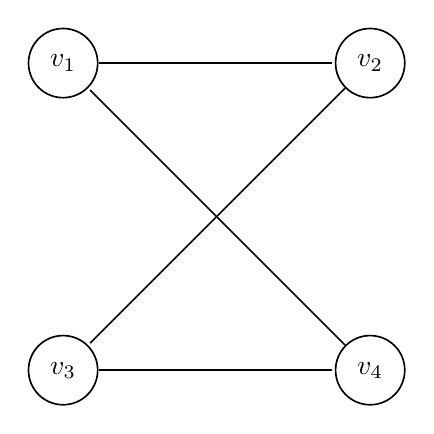
\begin{tikzpicture}[
    > = , % arrow head style
    shorten > = 1pt, % don't touch arrow head to node
    auto,
    node distance = 3cm, % distance between nodes
    semithick % line style
    ]

    \tikzset{every state}=[
    draw = black,
    thick,
    fill = black,
    minimum size = 1mm
    ]

    \node[state] (v1) {$v_1$};
    \node[state] (v2) [right=of v1] {$v_2$};
    \node[state] (v3) [below =of v1] {$v_3$};
    \node[state] (v4) [below =of v2] {$v_4$};
  
    \path[->] (v1) edge  node[]{}(v2);
    \path[->] (v2) edge  node[]{} (v3);
    \path[->] (v3) edge  node[]{}(v4);
    \path[->] (v4) edge  node[]{}(v1);
\end{tikzpicture}
\end{center}
{\normalfont{Using definition \ref{adjacent}, two adjacent vertices in }}G {\normalfont{are}} $v_1$ {\normalfont{and}} $v_2$.{\normalfont{ On the other hand, two non adjacent vertices in }}G {\normalfont{are}} $v_1$ {\normalfont{and}} $v_3.$\\ {\normalfont{By definition \ref{incident}}}, $v_1$ {\normalfont{and}} $v_2$ {\normalfont{are incident to the edge}} \{$v_1, v_2\}$.\\
{\normalfont{Using definition \ref{degree}, the degree of every vertex in}} G {\normalfont{is 2}}.
\end{example}
There are many important graphs in graph theory, one of them being the complete graph on $\mathit{n}$ vertices.
\begin{definition}
\label{Complete Graph}
A graph G(V,E) is said to be complete if $\forall$ v,w $\in$ V v $\neq$ w, v is adjacent to w. The complete graph on n vertices is denoted by $K_n$. \normalfont{\cite{harris_hirst_mossinghoff_2008}}
\end{definition}
Given any graph $\mathit{G(V,E)}$, one can also define graph theoretic structures that lie within $\mathit{G}$ such as walks and paths.
\begin{definition}
\label{walk}
Given a graph G(V,E), a walk is a sequence of vertices (not necessarily distinct) u= $u_1$, $u_2$, ...,$u_n$ = v such that $\forall$ i $\in$ [n-1], $\{u_i, u_{i+1}\}$ $\in$ E. Such a walk is usually referred to as a u-v walk, were u and v are the end vertices of the walk. \normalfont{\cite{harris_hirst_mossinghoff_2008}}
\end{definition}
\begin{definition}
\label{Path}
Given a graph G(V,E), a path in G joining any 2 vertices u, v $\in$ V, is a u-v walk with no repeated vertices.
\end{definition}
Definition \ref{Path} can now be used to define cycles and connectivity in a graph.
\begin{definition}
\label{connectedgraph}
A graph G(V,E) is said to be connected if $\forall$ u,v $\in$ V u $\neq$ v, u and v are joined by a path. \normalfont{\cite{harris_hirst_mossinghoff_2008}}
\end{definition}
\begin{definition}
\label{cycle}
Given a graph G(V,E), a cycle in G is a path $u_1$, ..., $u_k$ together with the edge \{$u_1, u_k\}$, where k $\geq$ 3 \normalfont{\cite{harris_hirst_mossinghoff_2008}}. 
\end{definition}
By Definitions \ref{walk} and \ref{Path} above, it is clear that a path is a special instance of a walk. Similarly, from Definitions \ref{Path} and \ref{cycle}, a cycle is a special instance of a path, with the only difference being that in a cycle, the first vertex and the last vertex are equal. Another thing worth mentioning is that, since according to definitions \ref{walk}, \ref{Path} and \ref{cycle}, cycles and paths are formulated in terms of walks, then they could only be perceived as sequences of vertices and not actual graphs. However, this is not the case because cycles and paths can be represented easily as graphs. For example, given the path/cycle $\mathit{u_1, u_2, ...,u_n}$, a new graph $\mathit{G(V,E)}$ can be created such that, $\mathit{V= \{ u_1, u_2, ..., u_n\}}$ and $\mathit{E = \{ \{u_i, u_{i+1}\} : \forall i, 0 < i < n\}}$. For example, consider the cycle $v_1$, $v_2$, $v_3$, $v_4$, $v_1$, then the graph depicted in example \ref{Example 1}, is the graph representing this cycle. Such graphs are known as Cycle/Path graphs and are denoted by $\mathit{C_n/P_n}$ respecitvely, $\mathit{n}$ being the number of vertices in the graph. Since this construction can be done, cycles/paths will be treated as both graphs and sequences throughout this dissertation. The usefulness of this remark will be seen when defining Hamiltonian cycles. Example \ref{example3} is constructed for better understanding of Definitions \ref{Complete Graph}, \ref{Path}, \ref{connectedgraph} and \ref{cycle}.
\begin{example}
\label{example3}
{\normalfont{Consider the graph}} G(V,E) {\normalfont{below:}}\\
\begin{center}
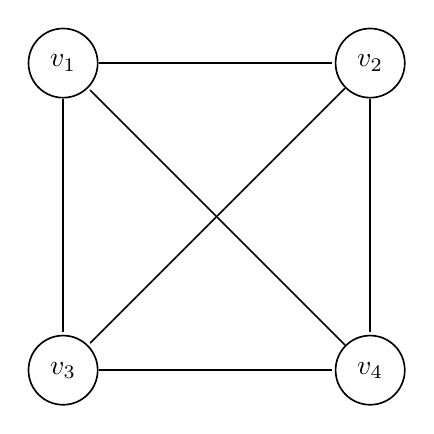
\begin{tikzpicture}[
    > = , % arrow head style
    shorten > = 1pt, % don't touch arrow head to node
    auto,
    node distance = 3cm, % distance between nodes
    semithick % line style
    ]

    \tikzset{every state}=[
    draw = black,
    thick,
    fill = black,
    minimum size = 1mm
    ]

    \node[state] (v1) {$v_1$};
    \node[state] (v2) [right=of v1] {$v_2$};
    \node[state] (v3) [below =of v1] {$v_3$};
    \node[state] (v4) [below =of v2] {$v_4$};
  
    \path[->] (v1) edge  node[]{}(v2);
    \path[->] (v1) edge  node[]{}(v3);
    \path[->] (v2) edge  node[]{} (v3);
    \path[->] (v3) edge  node[]{}(v4);
    \path[->] (v2) edge  node[]{}(v4);
    \path[->] (v4) edge  node[]{}(v1);
\end{tikzpicture}
\end{center}
{\normalfont{Since every vertex in}} G {\normalfont{is adjacent to every other vertex, then by Definition \ref{Complete Graph}, }}G {\normalfont{must be complete. Hence,}} G {\normalfont{must be}} $K_4$. {\normalfont{Since}} G {\normalfont{is complete, it must also be connected because, there is a path}} $P_2$ {\normalfont{between any two distinct vertices of}} G.\\
{\normalfont{Some examples of walks in}} G {\normalfont{are:}}\\
1. $v_1$ $v_2$ $v_3$ $v_4$ $v_1$ $v_2$\\
2. $v_1$ $v_4$ $v_2$ $v_3$ $v_1$ $v_3$\\
3. $v_4$ $v_3$ $v_1$ $v_4$ $v_1$\\
{\normalfont{Some examples of paths in}} G {\normalfont{are:}}\\
1. $v_1$ $v_2$ $v_3$ $v_4$\\
2. $v_1$ $v_4$\\
3. $v_4$ $v_3$ $v_1$\\
{\normalfont{Some examples of cycles in}} G {\normalfont{are:}}\\
1. $v_1$ $v_2$ $v_3$ $v_4$ $v_1$\\
2. $v_1$ $v_4$ $v_2$ $v_3$ $v_1$\\
3. $v_4$ $v_3$ $v_1$ $v_4$
\end{example}
 Another important graph theoretic concept is that of subgraphs. 
\begin{definition}
\label{subgraph}
Given a graph G(V,E) and a graph H($V^\prime$,$E^\prime$), H is a subgraph of G if $V^\prime$ $\subseteq$ V and $E^\prime$ $\subseteq$ E \normalfont{\cite{harris_hirst_mossinghoff_2008}}.
\end{definition}
Clearly, by definition \ref{subgraph} and the construction of Cycle/Path graphs, if $A$ is a cycle/path in $G$ then the Cycle/Path graph representing $A$ is a subgraph of $G$. This observation helps to define the concept of two distinct path/cycles. Two paths/cycles in $G$ are said to be distinct if, when they they are constructed as Path/Cycle subgraphs of $G$ they differ in at least one edge. After defining some important concepts, the next step is to extend Definition \ref{Graph} to define another important class of graphs called weighted graphs. It must also be noted that all definitions presented so far apply also to weighted graphs.
\begin{definition}
\label{Weighted Function}
Given a graph G(V,E), a weight function is a function f : E $\mapsto$ $\real^+$ {\normalfont{\cite{harris_hirst_mossinghoff_2008}}}. The real numbers assigned to each edge are called weights.
\end{definition}
Note that in Definition \ref{Weighted Function}, the weights are taken to be positive. According to \cite{harris_hirst_mossinghoff_2008}, there could be cases where negative weights would be appropriate, however in this dissertation it is to be assumed that when considering a weight function, the weights are positive.
\begin{definition}
\label{Weighted Graph}
A weighted graph is a graph G(V,E) with a weight function f {\normalfont{\cite{harris_hirst_mossinghoff_2008}}}. This will be denoted by the triple G(V,E,f) or G. 
\end{definition}
According to Bondy and Murty \cite{bondy_murty_1982}, weighted graphs occur regularly in applied graph theory. For example, a railway network can be represented by a weighted graph where the vertices are the set of towns in the railway network, and two vertices are connected if there is a direct route using the railway from one town to another, without visiting other towns in the process. The weight function would then represent the cost of travelling directly from one town to another. In addition to this, the shortest path between two towns in the network may be required. It is clear that in order to try and solve such problems, the total weight of a subgraph must first be defined.
\begin{definition}
\label{weightofasubgraph}
Given a weighted graph G(V,E,f), the total weight of any subgraph  H($V^\prime$,$E^\prime$,f) of G is $\sum_{e \in E^\prime}^{} f(e) $ \normalfont{\cite{bondy_murty_1982}}.
\end{definition}
It is important to note that by Definition \ref{subgraph}, any weighted graph G is a subgraph of itself, therefore, it's weight can be calculated. This is highlighted in Example \ref{example4} below.
\begin{example}
\label{example4}
{\normalfont{Consider the weighted graph}} G(V,E,f) {\normalfont{such that,}} G(V,E) {\normalfont{ is the graph in Example \ref{example3} with the weight function}} f {\normalfont{defined below:}}\\
f(\{$v_1, v_2\}$) = 4\\
f(\{$v_1, v_3\}$) = 5\\
f(\{$v_2, v_3\}$) = 2\\
f(\{$v_3, v_4\}$) = 10\\
f(\{$v_2, v_4\}$) = 4\\
f(\{$v_4, v_1\}$) = 7\\
{\normalfont{Then by Definition \ref{Weighted Graph}, the graph below is a weighted graph}}.\\
\begin{center}
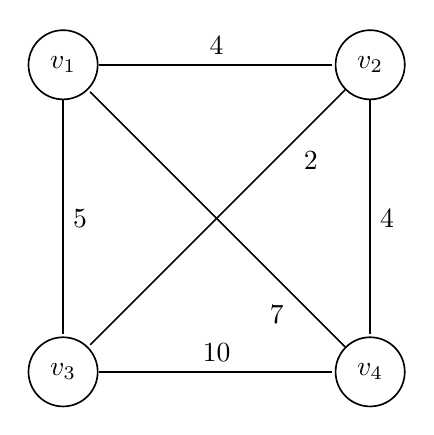
\begin{tikzpicture}[
    > = , % arrow head style
    shorten > = 1pt, % don't touch arrow head to node
    auto,
    node distance = 3cm, % distance between nodes
    semithick % line style
    ]

    \tikzset{every state}=[
    draw = black,
    thick,
    fill = white,
    minimum size = 1mm
    ]
    \node[state] (v1) {$v_1$};
    \node[state] (v2) [right=of v1] {$v_2$};
    \node[state] (v3) [below =of v1] {$v_3$};
    \node[state] (v4) [below =of v2] {$v_4$};
  
    \path[->] (v1) edge  node[]{4}(v2);
    \path[->] (v1) edge  node[]{5}(v3);
    \path[->] (v2) edge  node[pos=0.2,below right]{2} (v3);
    \path[->] (v3) edge  node[]{10}(v4);
    \path[->] (v2) edge  node[]{4}(v4);
    \path[->] (v4) edge  node[pos=0.2,below left]{7}(v1);
\end{tikzpicture}
\end{center}
 {\normalfont{As highlighted previously, the above graph is a subgraph of itself. Therefore, it's weight can be calculated. As a result, by Definition \ref{weightofasubgraph}, the weight of}} G {\normalfont{is 32.}}
\end{example}
According to Guichard \cite{guichard_2018}, trees are another useful class of graphs.
\begin{definition}
\label{tree}
A tree is a connected graph with no cycles \normalfont{\cite{guichard_2018}}.
\end{definition}
Having defined the basic building blocks in graph theory, it is now time to define harder concepts that use previous definitions. It is important to note that the following concepts can be applied to both weighted and unweighted graphs. Therefore, in the remaining definitions the graph being considered can either be weighted or unweighted.
\begin{definition}
\label{spanning subgraph}
H($V^\prime$,$E^\prime$) is a spanning subgraph of G(V,E) if H is a subgraph of G and $V^\prime$ = V \normalfont{\cite{ray_2013}}.
\end{definition}
There are many types of spanning subgraphs, however, the ones that are relevant to this dissertation are spanning trees and spanning cycles, the latter mostly known as Hamiltonian cycles.
\begin{definition}
A graph H is a spanning tree of G if H is a tree, and H is a spanning subgraph of G \normalfont{\cite{ray_2013}}.
\label{spanning tree}
\end{definition}
\begin{definition}
\label{hamiltonian cycle}
Given a graph G, C is a Hamiltonian cycle of G if C is a cycle, and C is a spanning subgraph of G. Also, a graph that contains a Hamiltonian cycle is called a Hamiltonian graph. \normalfont{\cite{ray_2013}}
\end{definition}
It is worth mentioning that Definition \ref{hamiltonian cycle} holds because, cycles can be represented by Cycle graphs due to the construction discussed earlier. What follows now is an example that illustrates better Definitions \ref{spanning subgraph}, \ref{spanning tree} and \ref{hamiltonian cycle}. 
\begin{example}
\label{example5}
{\normalfont{Let}} G {\normalfont{be the graph in Example \ref{example4}. Then, according to Definition \ref{spanning subgraph}, the two graphs below are two spanning subgraphs of}} G {\normalfont{because, they contain all the vertices of}} G {\normalfont{and are subgraphs of }}G .\\
\begin{center}
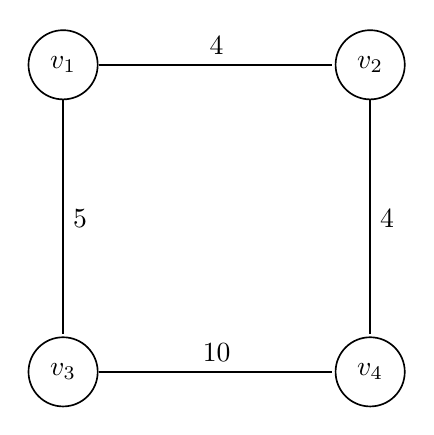
\begin{tikzpicture}[
    > = , % arrow head style
    shorten > = 1pt, % don't touch arrow head to node
    auto,
    node distance = 3cm, % distance between nodes
    semithick % line style
    ]

    \tikzset{every state}=[
    draw = black,
    thick,
    fill = white,
    minimum size = 1mm
    ]
    \node[state] (v1) {$v_1$};
    \node[state] (v2) [right=of v1] {$v_2$};
    \node[state] (v3) [below =of v1] {$v_3$};
    \node[state] (v4) [below =of v2] {$v_4$};
  
    \path[->] (v1) edge  node[]{4}(v2);
    \path[->] (v1) edge  node[]{5}(v3);
    \path[->] (v3) edge  node[]{10}(v4);
    \path[->] (v2) edge  node[]{4}(v4);
\end{tikzpicture}
\end{center}
\begin{center}
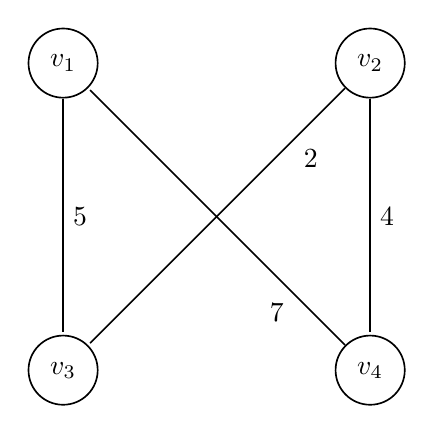
\begin{tikzpicture}[
    > = , % arrow head style
    shorten > = 1pt, % don't touch arrow head to node
    auto,
    node distance = 3cm, % distance between nodes
    semithick % line style
    ]

    \tikzset{every state}=[
    draw = black,
    thick,
    fill = white,
    minimum size = 1mm
    ]
    \node[state] (v1) {$v_1$};
    \node[state] (v2) [right=of v1] {$v_2$};
    \node[state] (v3) [below =of v1] {$v_3$};
    \node[state] (v4) [below =of v2] {$v_4$};
  
    \path[->] (v1) edge  node[]{5}(v3);
    \path[->] (v2) edge  node[pos=0.2,below right]{2} (v3);
    \path[->] (v2) edge  node[]{4}(v4);
    \path[->] (v4) edge  node[pos=0.2,below left]{7}(v1);
\end{tikzpicture}
\end{center}
{\normalfont{It must also be said that by Definition \ref{hamiltonian cycle}, the two graphs above are Hamiltonian cycles of}} G {\normalfont{because, they are spanning sub-graphs of}} G, {\normalfont{and are Cycle sub-graphs of}} G. {\normalfont{Since the above graphs are sub-graphs of }}G{\normalfont{, by Definition \ref{weightofasubgraph}, their weight can be calculated by summing up the weights of the edges. Thus, the Hamiltonian cycles above have weight 23 and 18 respectively.}}\\
{\normalfont{Given the graph }}G{\normalfont{ in Example \ref{example4}, the two graphs below are spanning trees of }}G{\normalfont{ of weight 18 and 19 respectively.}}\\
\begin{center}
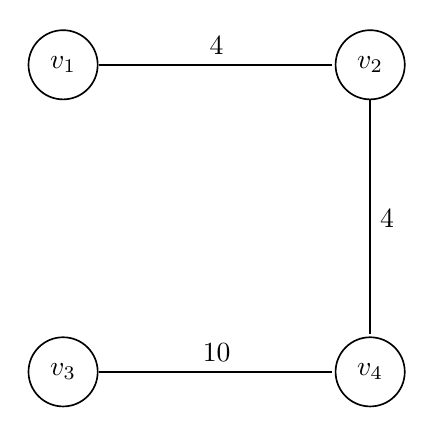
\begin{tikzpicture}[
    > = , % arrow head style
    shorten > = 1pt, % don't touch arrow head to node
    auto,
    node distance = 3cm, % distance between nodes
    semithick % line style
    ]

    \tikzset{every state}=[
    draw = black,
    thick,
    fill = white,
    minimum size = 1mm
    ]
    \node[state] (v1) {$v_1$};
    \node[state] (v2) [right=of v1] {$v_2$};
    \node[state] (v3) [below =of v1] {$v_3$};
    \node[state] (v4) [below =of v2] {$v_4$};
  
    \path[->] (v1) edge  node[]{4}(v2);
    \path[->] (v3) edge  node[]{10}(v4);
    \path[->] (v2) edge  node[]{4}(v4);
\end{tikzpicture}
\end{center}
\begin{center}
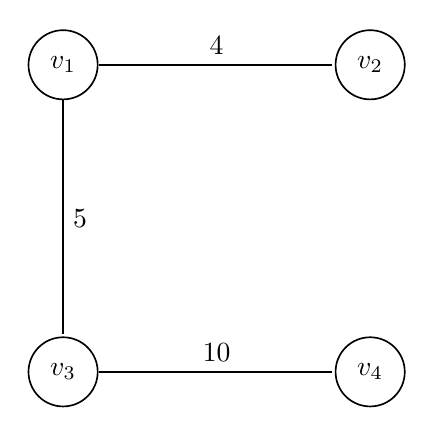
\begin{tikzpicture}[
    > = , % arrow head style
    shorten > = 1pt, % don't touch arrow head to node
    auto,
    node distance = 3cm, % distance between nodes
    semithick % line style
    ]

    \tikzset{every state}=[
    draw = black,
    thick,
    fill = white,
    minimum size = 1mm
    ]
    \node[state] (v1) {$v_1$};
    \node[state] (v2) [right=of v1] {$v_2$};
    \node[state] (v3) [below =of v1] {$v_3$};
    \node[state] (v4) [below =of v2] {$v_4$};
  
    \path[->] (v1) edge  node[]{4}(v2);
    \path[->] (v1) edge  node[]{5}(v3);
    \path[->] (v3) edge  node[]{10}(v4);
\end{tikzpicture}
\end{center}
{\normalfont{This example also shows that within the same weighted graph, there could be multiple Hamiltonian cycles and spanning trees of different weight.}}
\end{example}
Having defined Hamiltonian cycles and spanning trees, it is natural to ask whether there are necessary and sufficient conditions in a graph that guarantee it is Hamiltonian, or that it contains a spanning tree as sub-graph. In fact, Theorem \ref{spanningtreetheorem} gives a necessary and sufficient condition for a graph to have a spanning tree. Note that the proof of Theorem \ref{spanningtreetheorem} was constructed using ideas from \cite{ray_2013}.
\begin{theorem}
A graph G has a spanning tree $\iff$ it is connected {\normalfont{\cite{ray_2013}}}.
\label{spanningtreetheorem}
\end{theorem} 
\begin{proof}
($\implies$) Let $\mathit{G(V,E)}$ be a graph having a spanning tree $\mathit{T(V^\prime,E^\prime)}$ as one of it's subgraphs. Let $\mathit{v1, v2}$ $\in$ $\mathit{V}$. Since, $\mathit{T}$ is a spanning tree of $\mathit{G}$, then, $\mathit{T}$ is a spanning subgraph of $\mathit{G}$. Thus, $\mathit{v1, v2}$ $\in$ $V^\prime$. Also, since $\mathit{T}$ is a tree, $\mathit{T}$ must be connected. Therefore, $\exists$ a path $\mathit{P}$ joining vertices $\mathit{v_1}$ and $\mathit{v_2}$ in $\mathit{T}$. But since $\mathit{T}$ is a subgraph of G, then $\mathit{P}$ is also a path in $\mathit{G}$. Therefore $\mathit{G}$ must be connected.\\
($\Leftarrow$) Conversely, let $\mathit{G(V,E)}$ be a connected graph. Then, if $\mathit{G}$ has no cycles, $\mathit{G}$ itself must be a spanning tree. If $\mathit{G}$ has cycles, delete an edge from a cycle in $\mathit{G}$. Clearly, the resultant graph is still connected and contains one less cycle. Repeat this procedure untill no more cycles are left in the graph. Then, the resultant graph $\mathit{G^\prime}$ would be a connected subgraph of $\mathit{G}$ having no cycles (i.e a tree). Also, since by the deletion procedure no vertex was deleted from $\mathit{G}$, $\mathit{G^\prime}$ is a spanning subgraph of $\mathit{G}$. Therefore $\mathit{G^\prime}$ is a spanning tree of $\mathit{G}$.
\end{proof}
Theorem \ref{spanningtreetheorem} confirms that for a graph to have a spanning tree, the graph must be connected and vice-versa. Thus, for spanning trees, the necessary and sufficient condition is connectivity. However, the same cannot be said about Hamiltonian cycles because, no necessary and sufficient conditions are known for a graph to be Hamiltonian \cite{guichard_2018}. In fact, there are sufficient conditions for a graph to be Hamiltonian, however, these conditions are not necessary. There are also necessary conditions, some of which are trivial, such as, if $\mathit{G}$ is Hamiltonian then G must be connected, but this is not necessary and sufficient. According to Guichard \cite{guichard_2018}, these sufficient conditions typically say that for a graph to be Hamiltonian it must have a lot of edges. But, it is also argued in \cite{guichard_2018} that these conditions are not necessary because, there are Hamiltonian graphs that do not have many edges. For example, $\mathit{C_n}$ has only $\mathit{n}$ edges but is Hamiltonian. A sufficient but not necessary condition for Hamiltonianicity is Ore's Theorem below. Note that the proof of Theorem \ref{ore's theorem} was constructed using ideas from {\normalfont{\cite{ray_2013}}}.
\begin{theorem}[Ore's Theorem]
\label{ore's theorem}
Let G be a graph on n $\geq$ 3 vertices such that if v and w are not adjacent in G, then deg(v) + deg(w) $\geq$ n. Then G is Hamiltonian. {\normalfont{\cite{ray_2013}}}
\end{theorem}
\begin{proof}
Suppose that $\mathit{G(V,E)}$ is a graph satisfying all the conditions in the theorem statement, but is not Hamiltonian. Since $\mathit{G}$ is not Hamiltonian and $K_n$ is Hamiltonian, $\mathit{G}$ must be a subgraph of $\mathit{K_n}$ having fewer edges than $\mathit{K_n}$. Therefore, add edges to $\mathit{G}$ between non adjacent vertices to obtain a subgraph $\mathit{H(V^\prime,E^\prime)}$ of $\mathit{K_n}$, such that adding an edge to $\mathit{H}$ would create a subgraph of $\mathit{K_n}$ which is Hamiltonian. Let $\mathit{u, v}$ $\in$ $V^\prime$ be 2 non-adjacent vertices in H. Since by construction $\mathit{G}$ is a subgraph of $\mathit{H}$, $u$ and $v$ must be non-adjacent in $\mathit{G}$. Therefore, $\mathit{deg(u) + deg(v) \geq n}$ in both G and H. Since adding an edge to $\mathit{H}$ creates a resultant graph that is Hamiltonian, then, adding an edge between $\mathit{u}$ and $\mathit{v}$ creates a Hamiltonian graph. Therefore, in $\mathit{H}$ there must be a path joining $\mathit{u}$ and $\mathit{v}$ containing all the vertices of $\mathit{H}$. Let the path be $\mathit{u = v_1, v_2, ..., v_n = v}$.\\
Now, suppose $\mathit{deg(v_1)}$ = $\alpha$ in $\mathit{H}$. Now $\forall \mathit{i}, 1 <  i < \mathit{n}$, if there is an edge between $\mathit{v_1}$ and $\mathit{v_i}$ in $\mathit{H}$, then there must not be an edge between $\mathit{v_{i-1}}$ and $\mathit{v_n}$ because, $\mathit{v_1, v_i, v_{i+1}, ..., v_n, v_{i-1}, v_{i-2}, ..., v_1}$ would be a Hamiltonian cycle in $\mathit{H}$, thus H would be Hamiltonian. Therefore, $\mathit{deg(v_n)}$ $\leq$ $\mathit{n-1-\alpha}$\\
$\implies$ $\mathit{deg(v_1) + deg(v_n) \leq \alpha +  n-1 - \alpha}$ in $\mathit{H}$\\
$\implies$ $\mathit{deg(v_1) + deg(v_n) \leq n-1}$ in $\mathit{H}$\\
$\implies$ $\mathit{deg(v_1) + deg(v_n) < n}$ in $\mathit{G}$ since $\mathit{G}$ is a subgraph of $\mathit{H}$.\\
This contradicts the assumption that $\mathit{deg(v_1 = u) + deg(v_n = v) \geq n}$ in $\mathit{G}$ \\
Therefore, $\mathit{G}$ must be Hamiltonian.
\end{proof}
It is important to note that the above proof uses the fact that $K_n$ is Hamiltonian. This is true because, any cycle $C$ consisting of vertices from $K_n$ only is always a subgraph of $K_n$. Therefore, any cycle $C$ that spans $K_n$ is a spanning subgraph of $K_n$. Hence, by Definition \ref{hamiltonian cycle}, $C$ must be a Hamiltonian cycle of $K_n$, and therefore, $K_n$ is Hamiltonian. Example \ref{example 6} below is a counter example which shows why Ore's theorem gives a sufficient but not necessary condition.\\
\begin{example}
\label{example 6}
{\normalfont{Consider the graph}} $C_5$ below.
\\
\begin{center}
\begin{tikzpicture}[
    > = , % arrow head style
    shorten > = 1pt, % don't touch arrow head to node
    auto,
    node distance = 3cm, % distance between nodes
    semithick % line style
    ]

    \tikzset{every state}=[
    draw = black,
    thick,
    fill = white,
    minimum size = 1mm
    ]
    \node[state] (v1) {$v_1$};
    \node[state] (v2) [below left =of v1] {$v_2$};
    \node[state] (v3) [below right =of v1] {$v_3$};
    \node[state] (v4) [below=of v2] {$v_4$};
    \node[state] (v5) [below=of v3] {$v_5$};

    \path[->] (v1) edge  node[]{}(v2);
    \path[->] (v2) edge  node[]{}(v4);
    \path[->] (v4) edge  node[]{}(v5);
    \path[->] (v5) edge  node[]{}(v3);
    \path[->] (v3) edge  node[]{}(v1);
\end{tikzpicture}
\end{center}
$C_5$ {\normalfont{above is Hamiltonian because it contains the Hamiltonian cycle}} $v_1, v_2, v_4, v_5, v_3, v_1$. {\normalfont{However,}} deg($v_1$) + deg($v_5$) = 4 $<$ 5 = n. {\normalfont{Therefore, the condition in Ore's Theorem is not a necessary condition}}.
\end{example} 
The discussion in this section indicates that determining whether a graph is Hamiltonian is a very difficult problem. This means that there are certain problems that are harder than other problems. To formally reason about such problems, some computational theory must first be presented. This is done in the next section.
\subsection{Some Computational Theory}
\label{computational_theory}
After defining some important graph theoretic concepts, it is now time to present some important computational theory that will be used in the upcoming chapters. The discussion will now proceed by defining two different types of problems, and describing the relationship between them.
\begin{definition}
\label{optimization problems}
Suppose that a problem P has many possible solutions such that each solution has an associated value. Then, P is an optimization problem if P requires to find the solution with the best (minimum/maximum) value.  \normalfont{\cite{cormen_leiserson_rivest_stein}}
\end{definition}
Therefore, the aim of the algorithm solving an optimization problem is to find the solution with the best (minimum/maximum) value. A maximization problem is an optimization problem that requires to find the solution with the maximum value. On the other hand, a minimization problem is an optimization problem that requires to find the solution with the minimum value. A solution with the best value is called an optimal solution to the optimization problem being solved, and it's value is known as the optimal value. Note that an optimal solution is not termed as `the' optimal solution because, there could be many solutions having the same optimal value. Another type of problems area called decision problems. \cite{cormen_leiserson_rivest_stein}
\begin{definition}
\label{decision problems}
A Decision problems is a problem whose solution is either a yes or a no \normalfont{\cite{cormen_leiserson_rivest_stein}}.
\end{definition}
In \cite{cormen_leiserson_rivest_stein} it is argued that given an optimization problem, one can transform the given optimization problem into a decision problem, where the decision problem is easier to solve than the optimization problem. Therefore, if some optimization problem is easy to solve, the decision problem version is easy to solve as well \cite{cormen_leiserson_rivest_stein}. On the other hand, if the decision problem is hard to solve, then this would mean that the original optimization problem is also hard to solve \cite{cormen_leiserson_rivest_stein}. Note that the notion of `hard' and `easy' problems will be rigorously defined later in this section. This concept was only mentioned here to show that there exists a relationship between optimization problems and decision problems. Before going into harder computational theory, the example below is given to show how an optimization problem can be transformed into a related decision problem.
\begin{example}
\label{example decision/optimization}
{\normalfont{Two optimization problems are:\\
1. The Shortest Path Problem\\
2. The Minimum Weight Spanning Tree problem\\
Given a connected weighted graph}} G{\normalfont{ and two vertices $u$ and $v$ of $G$, the Shortest Path Problem is the task of finding a path}} P {\normalfont{between $u$ and $v$ in}} G {\normalfont{such that, the weight of }}P {\normalfont{is the minimum amongst all paths joining $u$ and $v$ in }}G {\normalfont{\cite{bondy_murty_1982}}}. {\normalfont{On the other hand, given a  connected weighted graph}} G {\normalfont{the Minimum Weight Spanning Tree Problem is the task of finding a spanning tree in}} G {\normalfont{of minimum weight \cite{harris_hirst_mossinghoff_2008}. The Shortest Path Problem is an optimization problem because, from all the possible paths joining $u$ and $v$ in the graph $G$, a path having the optimal value (minimum weight) joining $u$ and $v$ is chosen. In this case, the optimal solution is the path with minimum weight. Similarly, using the same reasoning, the minimum weight spanning tree problem is an optimisation problem. }}\\
{\normalfont{The decision problems related to the optimization problems above can be obtained by specifying a bound on the value to be optimized \cite{cormen_leiserson_rivest_stein}. Therefore, the decision problems related to the Shortest Path Problem and the Minimum Weight Spanning Tree Problem are the following:}}\\
{\normalfont{1. Given a connected weighted graph}} G, {\normalfont{two vertices}} u {\normalfont{and}} v, {\normalfont{and an integer}} k,{\normalfont{ does a path exist from}} u {\normalfont{to}} v {\normalfont{in}} G {\normalfont{of weight at most}} k?\\
{\normalfont{2. Given a connected weighted graph}} G, {\normalfont{and an integer}} k{\normalfont{, does}} G {\normalfont{contain a spanning tree of weight at most}} k?\\
{\normalfont{The two problems above are decision problems because the answer to these problems is either a yes or a no.}}
\end{example}
Reasoning about computational problems is usually done by analyzing the properties belonging to the algorithms that solve these problems. A common property which is analyzed is the running time of an algorithm. This is defined in Definition \ref{running_time} below.
\begin{definition}
\label{running_time}
The running time of an algorithm A given an input I is the number of steps executed by A when given I. The running time of an algorithm A can be represented by the function T $:$ $\mathbb{N}$ $\mapsto$ $\mathbb{N}$ where the domain represents the size of the input, and the co-domain represents the amount of steps executed by the algorithm, given an input size. {\normalfont{\cite{cormen_leiserson_rivest_stein}, \cite{adamchik_2009}}}
\end{definition}
What follows is an example which demonstrates how the running time of an algorithm can be computed.
\begin{example}
\label{example_running}
{\normalfont{Consider an algorithm that performs the addition of two}} n-{{\normalfont{bit strings. Then, if the addition of 2 bits takes}}} a {\normalfont{computational steps, the addition of 2}} $\mathit{n}${\normalfont{-bit strings will take}} a $\times$ n {\normalfont{steps, since, each computation must be performed}} n {\normalfont{times. Therefore, the running time of this algorithm for an input of size}} n {\normalfont{can be represented by the function,\\}} T(n) = a $\times$ n. {\normalfont{\cite{cormen_leiserson_rivest_stein}, \cite{adamchik_2009}}}
\end{example}
Expressing the running time in this way seems pretty easy to understand. However, this representation has a number of problems. Typically, the running time of an algorithm is fixed for any input, however, the running time function is not defined on the actual inputs, but, on the input sizes. As a result, since the same input size might represent different inputs, there could be different running times for the same input size $\mathit{n}$ as this depends on which input is given. This means that for any input size $\mathit{n}$, there may be different running time functions giving different running times. These different running time functions represent the different cases that could arise in an algorithm, given any input size $\mathit{n}$. The most important runnning time functions are the worst-case running time, the best-case running time, and the average-case running time. The worst/best/average case running time are the longest/shortest/average running time of an algorithm given any input of size $\mathit{n}$ respectively. Therefore, the problem is what running time function should be used to reason about algorithms. Although the average-case running time generally has a greater practical significance, it is often very difficult to compute. Therefore, the worst-case running time is usually used, that is, finding the running time function that gives the worst-case running time for any input of size $\mathit{n}$. The worst-case running time will be used because it is an upper bound to all other running times, therefore, this assures that the algorithm will never get a longer running time for any input of size $\mathit{n}$. So, if the worst case running time of an algorithm is polynomial in the input size, then it is known that the problem is in the class P (These terms will be defined later).  \cite{cormen_leiserson_rivest_stein}, \cite{adamchik_2009}\\\\
Another problem is that the running time of an algorithm can be difficult to compute precisely because, it depends on the computer the algorithm is executed on. This informally means that, an algorithm may need different amount of computational steps on different computers for the same input. For example, the number of steps taken for adding 2-bits as seen in Example \ref{example_running} may be different on different computers, resulting into running time functions that represent the same worst/best/average running time case, differing only in multiplicative constants and low order terms. To get around this problem, a mechanism that identifies a common property between all running time functions is needed. This mechanism is called asymptotic analysis. This means making the input size increase without bound so that only the order of growth of the running time function is relevant. This works because, as the input size increases, the low-order terms and multiplicative constants of the running time function get dominated by the size of the input itself. This means that, given any running time function, the low-order terms and multiplicative constants of the function can be ignored leaving only the order of growth (which is common across all running time functions representing the same best/worst/average running time case). In a running time function, the order of growth is given by the highest order term. This is true because, the highest order term has the greatest effect on the running time function as the input size increases. For example, given the running time function $\mathit{T(n) = an^2+bn+c}$, $\mathit{n^2}$ is the term that increases the running time the most, as the input size increases without bound. \cite{cormen_leiserson_rivest_stein}, \cite{adamchik_2009} \\\\
The following example is used to explain better what has been discussed in the previous paragraph.
\begin{example}
{\normalfont{Suppose that the}} n-{\normalfont{bit addition algorithm in Example \ref{example_running} has a worst-case running time function}} T(n) = a $\times$ n {\normalfont{on computer}} A, {\normalfont{and a worst-case running time function}} T(n) = b $\times$ n {\normalfont{on computer}} B {\normalfont{where,}} a/b {\normalfont{represent the number of computational steps required to perform 2-bit addition on computers}} A/B {\normalfont{respectively. The asymptotic analysis of the algorithm concludes that, the}} n-{\normalfont{bit addition algorithm has an }} $n$ {\normalfont{ asymptotic behaviour. Note that this is common to both running time functions}}. {\normalfont{\cite{cormen_leiserson_rivest_stein}, \cite{adamchik_2009}}}
\end{example}
To express the asymptotic behaviour of functions mathematically, asymptotic notations are normally used. One of these notations is called the Big O Notation, whose exact definition is given below.
\begin{definition}
\label{bigonotation}
Let f $:$ $\mathbb{N}$ $\mapsto$ $\mathbb{N}$ and g $:$ $\mathbb{N}$ $\mapsto$ $\mathbb{N}$ be two monotonic functions. Then, f(n) = O(g(n)) if $\exists$ c $>$ 0 and $n_0$ $>$ 0 such that f(n) $\leq$ cg(n) $\forall$ n $\geq$ $n_0$. \normalfont{\cite{adamchik_2009}} 
\end{definition}
Definition \ref{bigonotation} implicitly states that when writing $\mathit{f(n) = O(g(n)), g(n)}$ is an upperbound to $\mathit{f(n)}$ as the input size $\mathit{n}$ grows without bound \cite{adamchik_2009}. Therefore, if $\mathit{f(n)}$ is the worst case running time function of an algorithm and $\mathit{f(n) = O(g(n))}$, then it is guaranteed that as $\mathit{n \rightarrow \infty}$, the algorithm will never get a running time longer than $\mathit{g(n)}$ times some constant. Note that Definition \ref{bigonotation} can be used even for the asymptotic analysis of the average and best case running times. However, unless otherwise stated, it can be assumed that in this dissertation Big O Notation will be used for the worst-case asymptotic analysis of algorithms. The following is a continuation of Example \ref{example_running}.
\begin{example}
\label{bigonotationexample}
{\normalfont{By Example \ref{example_running}, the algorithm that performs two}} n-{\normalfont{bit addition has a running time function}} T(n)= an. {\normalfont{Therefore, by Definition \ref{bigonotation},}} T(n) = O(n) {\normalfont{because, since}} a  {\normalfont{is a natural number}} $\exists$ z $\geq$ a {\normalfont{such that,}} an $\leq$ zn $\forall$ n $\in$ $\mathbb{N}$. {\normalfont{Therefore at each step, the order of growth of}} T(n) {\normalfont{is linear with respect to the input size}} n.
\end{example}
It is important to note that if $\mathit{T(n) = O(g(n))}$, and $\mathit{h(n)}$ has a higher order of growth than $\mathit{g(n)}$, then, $\mathit{T(n) = O(h(n))}$. For example, in Example \ref{bigonotationexample} $\mathit{T(n) = O(n^2)}$ as well since $\mathit{n^2}$ is an upperbound to $\mathit{n}$, and hence, $n^2$ is an upperbound to $\mathit{T(n)}$. However, unless otherwise stated, it can be assumed that whenever $\mathit{T(n) = O(g(n))}$, $\mathit{g(n)}$ is a tight asymptotic bound to $\mathit{T(n)}$. A tight asymptotic bound to $\mathit{T(n)}$ is a function $\mathit{g(n)}$ such that if $\mathit{T(n)=O(f(n))}$, then $\mathit{g(n)=O(f(n))}$.\\\\
Given the above, the time complexity of an algorithm can now be defined formally.
\begin{definition}
\label{time_complexity}
Given a function g(n) and an algorithm A having a running time function T(n), A is said to have a time complexity of O(g(n)) if T(n) = O(g(n)). \normalfont{\cite{adamchik_2009}} 
\end{definition}
Definition \ref{time_complexity} does not apply only to the worst case running time function. However, recall that when discussing running time functions it was highlighted that it can be assumed that, the worst-case running time function is always taken. Therefore, it can be assumed that the worst-case running time function is taken when saying that an algorithm has an $\mathit{O(g(n))}$ time complexity, or when saying that an algorithm is an $\mathit{O(g(n))}$ algorithm. For clarity, this will sometimes also be termed as the `worst-case time complexity' of the algorithm. Note that when it is said that a problem can be solved in $\mathit{O(g(n))}$ time, this means that the problem can be solved by an algorithm that has an $\mathit{O(g(n))}$ worst-case time complexity.\\\\
The following table summarizes some of the most common time complexities encountered in computational theory, and what they are commonly known as. The table was adapted using information from \cite{pettis} and \cite{carter_1999}.
\begin{table}[!htbp]
  \begin{center}
    \caption{Time Complexities and Terminology Used.}
    \label{tab:table1}
    \begin{tabular}{l|c} % <-- Alignments: 1st column left, 2nd middle and 3rd right, with vertical lines in between
      \textbf{Time Complexity} & \textbf{Terminology Used}\\
      \hline
      O(1)                          & Constant time    \\
     $O(\mathit{\log n})$          & Logarithmic time \\
     $O(\mathit{n})$               & Linear time      \\
     $O(\mathit{n \log n})$        & Log-linear time  \\
     $O(\mathit{n^2})$             & Quadratic time   \\
     $O(\mathit{n^c})$, $\mathit{c > 0}$ constant & Polynomial time  \\
     $O(\mathit{a^n})$, $\mathit{a \geq 2}$ constant & Exponential time \\
     $O(\mathit{n!})$              & Factorial time
    \end{tabular}
  \end{center}
\end{table}
\\In Table \ref{tab:table1}, the time-complexities are ordered in ascending order of growth using the curves in \cite{rowell}. This means that for example constant time algorithms have a smaller order of growth than logarithmic time algorithms. It must be noted that the higher the order of growth of an algorithm is, the more steps the algorithm needs to execute for any input, and therefore, the less efficient the algorithm is. In general, problems that can be solved in polynomial time are tractable problems \cite{cormen_leiserson_rivest_stein}. On the other hand, problems that require super-polynomial (exponential/factorial) time algorithms to be solved are intractable problems \cite{cormen_leiserson_rivest_stein}. In general, tractable problems are considered to be easy to solve, whereas intractable problems are hard to solve. Table \ref{tab:table2} below is constructed to show why problems that can be solved in polynomial time are tractable, whilst, problems that cannot be solved in polynomial time are intractable. Table \ref{tab:table2} gives the execution time of any algorithm given an input of size $\mathit{10}$ or $\mathit{100}$, provided that the algorithm's time complexity is $\mathit{O(n)}$, $\mathit{O(n^2)}$, $\mathit{O(2^n)}$ or $\mathit{O(n!)}$.\\\\
\begin{table}[h]
  \begin{center}
    \caption{Execution Time Given Input Size and Time Complexity}
    \label{tab:table2}
    \begin{tabular}{l|c|c|c} % <-- Alignments: 1st column left, 2nd middle and 3rd right, with vertical lines in between
      \textbf{\backslashbox{Time Complexity}{Input Size}} & \textbf{10} & \textbf{100}\\
      \hline
&&\\
     $\mathit{O(n)}$ & $\mathit{3.171{\times10^{-16} years}}$ & $\mathit{3.171{\times10^{-15} years}}$\\
     $\mathit{O(n^2)}$ & $\mathit{3.171{\times10^{-15} years}}$ & $\mathit{3.171{\times10^{-13} years}}$     \\
     $\mathit{O(2^n)}$ & $\mathit{3.247{\times10^{-14} years}}$ & $\mathit{4.0197{\times10^{13} years}}$\\
     $\mathit{O(n!)}$ & $\mathit{1.1507{\times10^{-10} years}}$ & Very large to compute
    \end{tabular}
  \end{center}
\end{table}
\\Table \ref{tab:table2} above was adapted from \cite{pettis}. In Table \ref{tab:table2} above it is assumed that the machine the algorithms can be executed on perform $\mathit{10^9}$ computational steps per second, as in \cite{pettis}. It can be concluded from Table \ref{tab:table2} above that as the size of the input increases, only the polynomial functions have small values. This means that a polynomial time algorithm does not have a very large execution time even if the size of the input is increased substantially. On the other hand, an algorithm with an exponential or factorial time complexity has a very large execution time if the input size is large. This true because, the rate of growth of the time complexity function is very large. What follows is an example which wraps up all the time complexity concepts discussed so far.
\begin{example}
\label{time_complexity_example}
{\normalfont{In Example \ref{bigonotationexample},}} T(n) = O(n). {\normalfont{Therefore, according to Definition \ref{time_complexity}, the}} n-{\normalfont{bit addition algorithm has a time complexity of}} O(n). {\normalfont{Therefore by Table \ref{tab:table1}, the}} n-{\normalfont{bit addition algorithm has a linear time complexity, or simply is a linear time algorithm. As a result, the}} n-{\normalfont{bit addition problem can be solved in linear time, and hence in polynomial time.}}.
\end{example}
In what has been presented so far in this section, it has always been assumed that any problem has an algorithm that solves it. However, this is not the case because there are computational problems that cannot be solved by any computer, no matter how much processing power and time is dedicated to them. In addition to that, there are problems that can be solved in polynomial time and others which cannot. This seems to indicate that there are several classes of problems. In fact, one of these classes is the class P defined below. \cite{cormen_leiserson_rivest_stein}
\begin{definition}
\label{P}
The class P consists of all the problems that can can be solved in polynomial time {\normalfont{\cite{cormen_leiserson_rivest_stein}}}.
\end{definition}
Therefore, according to Definition \ref{P}, the class P consists of tractable problems. An example of a problem in the class $\mathit{P}$ is the $\mathit{n}$-bit addition problem defined in Example \ref{example_running}. The $\mathit{n}$-bit addition problem is in the class P because it can be solved in linear time (as Discussed in Example \ref{time_complexity_example}). Apart from the class P, there is also the class NP. The following two definitions help in defining the class NP. Note that Definition \ref{certificate} was adapted from information in \cite{kaveh_tehada_2013}.
\begin{definition}
\label{certificate}
A certificate of a solution is a mathematical object that guarantees the solution.
\end{definition}
It can be deduced from Definition \ref{certificate} that if a certificate is correct, then the solution is correct. Therefore, one can verify if a given solution is correct by actually verifying that the certificate is correct. For convenience, in this dissertation, `verifying a solution/certificate if it is correct' will be referred to as `verifying a solution'. Note that Definition \ref{certificate} is not the exact mathematical definition of a certificate. The exact mathematical definition of a certificate is not given because, it requires discussing concepts about languages and verification algorithms which are beyond the scope of this project. A more formal discussion about certificates is given in \cite{cormen_leiserson_rivest_stein}.
\begin{definition}
\label{polynomial_time_verification}
Suppose that S is an arbitrary solution to a problem A. Then, A can be verified in polynomial time if given a certificate C of S, $\exists$ a polynomial time algorithm such that, when supplied C and an instance (input) of A as inputs, the algorithm can verify if C is correct. {\normalfont{\cite{cormen_leiserson_rivest_stein}}}
\end{definition}
In other words, Definition \ref{polynomial_time_verification} states that, a problem can be verified in polynomial time if the certificate that lead to the solution can be verified by a polynomial time algorithm. Note that as discussed before, when verifying a certificate, the solution is implicitly verified. What follows now is an example that explains Definition \ref{certificate} and Definition \ref{polynomial_time_verification}.
\begin{example}
\label{example_polynomial_time_verification}
{\normalfont{To explain Definition \ref{certificate} and Definition \ref{polynomial_time_verification}, the Hamiltonian Cycle problem is going to be used. Given a graph}} G(V,E){\normalfont{, the Hamiltonian cycle problem is the task of determing whether}} G {\normalfont{has a Hamiltonian cycle \cite{cormen_leiserson_rivest_stein}. A certificate of a solution to the Hamiltonian cycle problem can be a sequence of distinct vertices}} S = $v_1$, ..., $v_n$ {\normalfont{on }}$|$V$|$ = n {\normalfont{vertices. Note that if the solution to a Hamiltonian cycle problem instance is `yes' then, the certificate would guarantee the solution if it is a Hamiltonian cycle in}} G{\normalfont{. On the other hand, if the solution to the Hamiltonian cycle problem is a `no', then, any certificate given guarantees the solution. The solution is guaranteed when the answer is `no' because, since there is no Hamiltonian cycle in}} G{\normalfont{, there is no certificate that represent a Hamiltonian cycle in}} G{\normalfont{. As a consequence of these observations, for the Hamiltonian cycle problem to be verifiable in polynomial time, there must be a polynomial time algorithm that checks whether the certificate is a Hamiltonian cycle when the answer is `yes'. This can be done by creating an algorithm that checks if }} $\forall$ i $\in$ [n-1], \{$v_i, v_{i+1}\} \in$ E and \{$v_n$, $v_1\} \in$ E. {\normalfont{Therefore, the checker algorithm has a worst case}} O(n) {\normalfont{time complexity because, it must check all edges in the cycle. Hence, the checker algorithm takes polynomial time to execute. As a result, the Hamiltonian cycle problem can be verified in polynomial time.}}
\end{example}
Note that, as shown in Example \ref{example_polynomial_time_verification}, to show that a problem is verifiable in polynomial time, it is only needed to be shown that a certificate of the solution `yes' can be verified in polynomial time'. This is because, any certificate is correct when the answer is `no'. Now the class NP can be defined.
\begin{definition}
\label{NP}
The class NP consists of all decision problems that can be verified in polynomial time {\normalfont{\cite{cormen_leiserson_rivest_stein}, \cite{dorigo_stutzle_thomas_2004}}}.
\end{definition}
 It is important to note that according to Definition \ref{NP}, a problem $\mathit{A}$ is in the class NP if $\mathit{A}$ is a decision problem. This will not be a limiting factor because, as discussed before, every optimization problem can be transformed into a related decision problem by specifying a bound on the solution to be optimized (see Example \ref{example decision/optimization}). Reasoning about decision problems is easier because, the related decision problem is not harder than the original optimization problem. As a result, one can prove that an optimization problem cannot be solved in polynomial time by showing that, the related decision problem cannot be solved in polynomial time.\cite{cormen_leiserson_rivest_stein}\\\\
Another important class of problems is the class of NP-Complete problems. To define this class, the concept of a reduction algorithm must first be defined.
\begin{definition}
\label{reduction_algorithm}
Suppose that A and B are two decision problems. A reduction algorithm is an algorithm that transforms any instance $\alpha$ of A into an instance $\beta$ of B with the following properties:
\begin{itemize}
   \item The algorithm takes polynomial time to execute
   \item The solution to $\alpha$ is yes $\iff$ the solution to $\beta$ is yes.
\end{itemize} 
For convenience, if there exists a reduction algorithm R which transforms any instance $\alpha$ of $A$ into an instance $\beta$ of $B$, then it will be said that `R transforms A to B' or `A is reducible to B'. {\normalfont{\cite{cormen_leiserson_rivest_stein}}}
\end{definition}
A reduction algorithm has important applications in computational theory. In fact, suppose that there are two decision problems $\mathit{A}$ and $\mathit{B}$ such that an instance $\mathit{\alpha}$ of the problem $\mathit{A}$ needs to be solved in polynomial time. Suppose also that $\mathit{B}$ can be solved in polynomial time using algorithm $\mathit{B^\star}$, and there exists a reduction algorithm $\mathit{R}$ from $\mathit{A}$ to $\mathit{B}$. Then, $\mathit{A}$ can be solved in polynomial time in the following way :
 \begin{itemize}
	\item Use $\mathit{R}$ to transform $\mathit{\alpha}$ into an instance $\mathit{\beta}$ of $\mathit{B}$
	\item Execute $\mathit{B^\star}$ on the input $\beta$ to get answer $\gamma$ = yes/no
	\item Give $\mathit{\gamma}$ as an answer for $\mathit{\alpha}$.
\end{itemize} 
It is important to note that $\mathit{A}$ can be solved in polynomial time because the total time of the above procedure is polynomial. The above procedure is polynomial because, the total time of executing two polynomial time algorithms is the summation of two polynomials, which by properties of polynomials is still polynomial. It is important to note that, the above could only be done because the solution to $\alpha$ is yes $\iff$ the solution to $\beta$ is yes. \cite{cormen_leiserson_rivest_stein}\\\\
Another important application of reduction algorithms is to show that a polynomial time algorithm does not exist for a particular decision problem. Let $\mathit{A}$ and $\mathit{B}$ be decision problems such that $\mathit{A}$ cannot be solved in polynomial time. Suppose that $\exists$ a reduction algorithm $\mathit{R}$ from $\mathit{A}$ to $\mathit{B}$. Then it can be shown that $\mathit{B}$ cannot be solved in polynomial time because, if $\mathit{B}$ can be solved in polynomial time, then $\mathit{R}$ can be used to transform any instance $\alpha$ of $\mathit{A}$ into an instance $\beta$ of $\mathit{B}$ where again, $\alpha$ can be solved in polynomial time as discussed in the previous paragraph. Since $\alpha$ is arbitrary, $\mathit{A}$ can be solved for all inputs in polynomial time and hence, $\mathit{A}$ can be solved in polynomial time. This contradicts the assumption that $\mathit{A}$ cannot be solved in polynomial time. Therefore, when using a reduction algorithm from a decision problem $\mathit{A}$ to a decision problem $\mathit{B}$, one implicitly makes the statement that decision problem $\mathit{B}$ is as hard (in terms of tractability as discussed before) as decision problem $\mathit{A}$. If not, this would contradict properties that belong to the problem $\mathit{A}$. After defining reduction algorithms, the class of NP-Complete problems can now be defined. \cite{cormen_leiserson_rivest_stein}
\begin{definition}
\label{NPC}
A decision problem A is in the class NP-Complete (NPC) if A is in NP, and A is as hard as any problem in NP {\normalfont{\cite{cormen_leiserson_rivest_stein}} }.
\end{definition}
In other words, Definition \ref{NPC} states that for a problem $\mathit{A}$ to be in the class NPC, $\mathit{A}$ must be in NP, and that any problem in NP can be transformed using a reduction algorithm into $\mathit{A}$. Therefore, to show that a problem $\mathit{A}$ is in NPC, one must show that it is in NP, and that every problem in NP can be reduced to $\mathit{A}$. Showing that $\mathit{A}$ is in NP is not difficult because, it only requires to show that an alleged solution for an instance of A can be verified in polynomial time. As discussed before, this can be done by checking that a certificate for the solution `yes' can be verified in polynomial time. On the other hand, showing that every problem in NP is reducible to $\mathit{A}$ may seem difficult because, this requires checking that every problem in NP can be reduced to $\mathit{A}$. However, this is not the case because by Exercise 34.3-2 in \cite{cormen_leiserson_rivest_stein}, reduction algorithms are transitive. Hence, considering a known NP-Complete problem $\mathit{H}$, since $\mathit{H}$ is NP-Complete, every problem in NP can be reduced to $\mathit{H}$. Therefore, if a reduction algorithm from $\mathit{H}$ to $\mathit{A}$ can be found, then by transitivity of reduction algorithms, every problem in NP can be reduced to $\mathit{A}$ using a reduction algorithm \cite{cormen_leiserson_rivest_stein}.\\\\
The classes P, NP and NPC have very important implications in computational theory. One of the most important problems in computational theory is whether P = NP. It is known that P $\subseteq$ NP. This is true because, since every problem in P can be solved in polynomial time, then implicitly the polynomial time verification has been done by the algorithm solving the problem (because it is guaranteed that the algorithm gives a correct solution in polynomial time). Note that to be precise, the problems in P must first be converted to a related decision problem if they are to be in NP. But since this can be done, and the related decision problem is no harder than the original problem, the result holds. Therefore, every problem in P is in NP and hence, P $\subseteq$ NP. Showing that NP $\subseteq$ P may seem to be easy as well. In fact, to show that NP $\subseteq$ P, it must be shown that $\exists$ an NP-Complete problem $\mathit{C}$ that can be solved in polynomial time. This would be enough because, by the NP-Completeness of $\mathit{C}$, every problem in NP can be reduced using a reduction algorithm to $\mathit{C}$ and hence, every problem in NP could be solved in polynomial time since the reduction algorithm and the algorithm solving $\mathit{C}$, would take a total time that is still polynomial. Unfortunately, no polynomial time algorithm has yet been discovered for any problem in NPC. In addition to this, no one has yet been able to prove that such polynomial time algorithms do not exist for NP-Complete problems. This essentially means that the NP $\subseteq$ P problem is still an open question. \cite{cormen_leiserson_rivest_stein}\\\\
It is important to note that as indicated in \cite{dorigo_stutzle_thomas_2004}, the classes P, NP and NPC are usually defined more formally using models of computations such as Turing Machines. This was not done in this way because Turing Machines are out of the scope of this dissertation. For a more formal definition of these classes, the reader can find more information in \cite{garey_johnson_1979}.\\\\
After defining the computational theory required, it is now time to mathematically define the Travelling Salesman Problem, and present some important properties about it. This will lead to showing that the Travelling Salesman Problem is NP-Complete, hence, showing that no polynomial time algorithm which solves the Travelling Salesman Problem has been discovered yet. All of this will be done in the next chapter.
\newpage
{\center{\section{The Travelling Salesman Problem} \label{TSP_CHAPTER}}}
As discussed in Chapter \ref{introduction}, this chapter is divided into two main sections. In the first section, the Travelling Salesman Problem will be mathematically defined, and some properties about it will be discussed. This will lead to showing that the Travelling Salesman Problem is in NPC. As a result, by the discussion in Section \ref{computational_theory}, no polynomial time algorithm which solves the Travelling Salesman Problem is known. According to \cite{cormen_leiserson_rivest_stein}, this does not mean that the Travelling Salesman Problem cannot be approximated in polynomial time. Hence in the second section, two algorithms that can approximate the Travelling Salesman Problem in polynomial time will be presented, along with some theoretical results about them.
\subsection{Problem Definition, Properties and Complexity Class}
The Travelling Salesman Problem can be defined mathematically as follows.
\begin{definition}
\label{TSP}
Given a complete weighted graph G on at least three vertices, the Travelling Salesman Problem (TSP) is the problem of finding a minimum weight Hamiltonian cycle in G {\normalfont{\cite{bondy_murty_1982}}}.
\end{definition}
According to Definition \ref{TSP}, a weighted graph $\mathit{G}$ must be complete for the TSP to be defined. However, this is not a limiting factor because, every weighted graph $\mathit{G^\prime}$ can be converted into a complete weighted graph, by adding the missing edges in $\mathit{G^\prime}$ with a very large weight. Note that this can be done because, if $\mathit{G^\prime}$ is an incomplete weighted Hamiltonian graph, the minimum weight Hamiltonian cycle in $\mathit{G^\prime}$ would never be effected when transforming $\mathit{G^\prime}$ into a complete graph in this way. The minimum weight Hamiltonian cycle can never be effected because, since the missing edges have a very large weight, they can never be part of the minimum weight Hamiltonian cycle when added. Therefore, since incomplete weighted graphs can be represented as complete weighted graphs, it can be assumed that complete weighted graphs are always being considered when discussing the TSP.\\\\
Definition \ref{TSP} also assumes indirectly that if $\mathit{G}$ is a complete weighted graph, then $\mathit{G}$ is Hamiltonian. This is true because, any 2 distinct vertices in $K_n$ are adjacent, therefore, every Hamiltonian cycle consisting of $n$ vertices must be in $K_n$. Note that for the TSP, $K_2$ and $K_1$ are implicitly excluded because by Definition \ref{cycle}, cycles are defined on graphs having at least 3 vertices. The following example is used to clearly explain what the TSP defined in Definition \ref{TSP} is all about.
\begin{example}
\label{example_2.1}
{\normalfont{Consider the complete graph}} $K_4$ {\normalfont{with the weight function}} f {\normalfont{defined in Example \ref{example4}. The distinct Hamiltonian cycles of}} G {\normalfont{are:}}
\begin{itemize}
   \item $v_1$, $v_2$, $v_3$, $v_4$, $v_1$ {\normalfont{with weight}} 23
   \item $v_1$, $v_3$, $v_4$, $v_2$, $v_1$ {\normalfont{with weight}} 23
   \item $v_1$, $v_3$, $v_2$, $v_4$, $v_1$ {\normalfont{with weight}} 18
\end{itemize} 
{\normalfont{Therefore, by Definition \ref{TSP}, the solution of the TSP given the graph in Example \ref{example4} would be the minimum weight Hamiltonian cycle}} $v_1$, $v_3$, $v_2$, $v_4$, $v_1$. {\normalfont{Note that $K_4$ has three distinct Hamiltonian cycles. This fact is a special case of Lemma \ref{distinct_hamiltonian_cycles} for any $K_n$}}. 
\end{example}
Example \ref{example_2.1} suggests implicitly that to solve the TSP on any complete weighted graph, one can do it by a brute-force algorithm. A brute-force algorithm for the TSP is one that computes all the Hamiltonian cycles in a graph, and chooses the one of least weight as a solution \cite{Sanchit}. However, $\mathit{K_n}$ contains $\mathit{\frac{(n-1)!}{2}}$ distinct Hamiltonian cycles. Therefore, a brute-force algorithm is inefficient because, it must generate all the distinct Hamiltonian cycles in the graph taking factorial time to do so \cite{Sanchit}. 
\begin{lemma}
\label{distinct_hamiltonian_cycles}
For n $\geq$ 3, $K_n$ has $\frac{(n-1)!}{2}$ distinct Hamiltonian cycles {\normalfont{\cite{Sanchit}}}. 
\end{lemma}
\begin{proof}
Suppose that $V$ and $E$ are the set of vertices and the set of edges of $K_n$ respectively. Any Hamiltonian cycle in $K_n$ can be represented by a permutation of $V$ and vice-versa. For example the Hamiltonian cycle $h$ = $v_1$, ..., $v_n$, $v_1$ can be represented by the permutation $v_1$ $v_2$ ... $v_n$ and vice-versa. Therefore, the number of Hamiltonian cycles in $K_n$ is equal to the number of permutations of $V$. Since there are $n!$ permutations of $V$, there must be $n!$ Hamiltonian cycles in $K_n$. Now, in terms of Hamiltonian cycles, $h$, is the same as the Hamiltonian cycle $v_2$, ..., $v_n$, $v_1$, $v_2$. This is true because, although the order of vertices is different, they use the same edges from $E$. Therefore, in general there are $n$ distinct permutations (one for every vertex in $K_n$ when used as a starting vertex of the vertex sequence) representing the same Hamiltonian cycle. In addition to this, each permutation would still represent the same Hamiltonian cycle if the vertices are in reversed order. This is true because, again the same edges from $E$ are used. Therefore, there must be $\frac{n!}{2n}$ = $\frac{(n-1)!}{2}$ distinct Hamiltonian cycles in $K_n$.
\end{proof}
As discussed previously, Lemma \ref{distinct_hamiltonian_cycles} confirms that a brute-force algorithm is not efficient enough to solve the TSP for large inputs. This means that either a new algorithm that solves the TSP in polynomial time must be designed, or it can be shown that the TSP is in NPC. As discussed in Section \ref{computational_theory}, the latter would confirm that no polynomial time algorithm is known for the TSP. It is important to note that, this does not mean that TSP cannot be solved in polynomial time.\\\\ In what follows, it will be proven that the TSP is an NP-Complete problem. Therefore, first it will be shown that TSP is in NP, and secondly it will be shown that TSP is as hard as any problem in NP. It is important to note that to prove that TSP is in NP, the TSP defined in Definition \ref{TSP} must be converted into a related decision problem. This is needed because in Definition \ref{TSP}, the TSP was presented as an optimization problem, and because, by Definition \ref{NP}, the class NP contains decision problems only. The TSP's related decision problem is the following :
\begin{definition}[TSP defined as a decision problem]
\label{dec_prob}
Given an instance $(G,k)$ where $G$ is a complete weighted graph and $k$ is an integer, does $G$ contain a Hamiltonian cycle of weight at most $k$ \cite{cormen_leiserson_rivest_stein}?
\end{definition}
Having converted the TSP in Definition \ref{TSP} into a related decision problem, it is now time to show that TSP is in NP. This is shown in Lemma \ref{TSP_in_NP} below. Note that the proof of Lemma \ref{TSP_in_NP} was constructed using ideas in \cite{cormen_leiserson_rivest_stein}.
\begin{theorem}
\label{TSP_in_NP}
TSP is in NP {\normalfont{\cite{cormen_leiserson_rivest_stein}}}.
\end{theorem}
\begin{proof}
Consider the TSP's decision problem variant. To show that TSP is in NP, it must be shown that an alleged solution for the TSP can be verified in polynomial time. As discussed in Section \ref{computational_theory}, this can be done by verifying in polynomial time a certificate for the solution `yes'. Suppose that $G(V,E)$ is a complete weighted graph on $n$ vertices. A certificate of a solution to the TSP given G can be a sequence of $n$ vertices. Suppose that $v_1$, $v_2$, ..., $v_n$ is an arbitrary certificate. To check that the certificate is correct, two checks on this certificate must be carried out by an algorithm. Firstly, the algorithm must check that no vertex in the certificate is repeated (i.e. that the certificate is a Hamiltonian cycle). Secondly, the algorithm must check that, the total weight of the Hamiltonian cycle obtained from the certificate is at most $k$. Therefore, the algorithm is made up of the following two parts:
\begin{itemize}
   \item In the first part, the algorithm must check that for all $i$ $\in$ [$n$], $v_i$ appears only once in the certificate. This part of the algorithm can be implemented by keeping an array $A$ of boolean values having length $n$ such that, for each $v_i$, the algorithm checks that $A[i]$ is $0$. If $A[i]$ is set to $0$, the algorithm sets $A[i]$ to $1$ when it encounters $v_i$ in the given sequence and then moves to the next vertex in the solution sequence. If while traversing the certificate, the checker algorithm notices that for $j$ $\in$ [$n$], $A[j]$ has already been set to 1, the algorithm stops because this means that, $v_j$ is repeated and hence the certificate is not a Hamiltonian cycle. As a result, the certificate is incorrect. If this does not happen, the algorithm starts executing the next part (next bullet point). Clearly, this first part of the algorithm has a worst-case $O(n)$ time complexity were $n$ is the length of the solution sequence. The worst-case occurs when the checker algorithm needs to traverse all the vertices in the solution sequence. As a result, this part of the checker algorithm can be executed in polynomial time.
   \item The checker algorithm must now check that, the total weight of the Hamiltonian cycle represented by the sequence of vertices is at most $k$ . This part of the checker algorithm can be implemented by keeping a floating point variable named `total\_weight', and summing the weight of each edge used in the Hamiltonian cycle to the variable `total\_weight'. Since a Hamiltonian cycle contains $n$ edges, this part of the checker algorithm has a worst-case $O(n)$ time complexity because, all edges must be summed to calculate the total weight of the Hamiltonian cycle. After the total weight of the solution sequence is calculated, it is checked in $O(1)$ time whether `total\_weight' $\leq k$. If this inequality is satisfied, the checker algorithm declares the solution as correct, otherwise declares the solution as incorrect. Therefore, it can be concluded that, this part of the checker algorithm has an $O(n)$ worst-case time complexity. Hence, this part of the checker algorithm can be executed in polynomial time.
\end{itemize} 
Since the checker algorithm is made up of two parts that execute in polynomial time, then, the whole algorithm runs in polynomial time. Therefore, it can be concluded that, any certificate can be verified if it is correct or not in polynomial time by the above checker algorithm. Therefore, the TSP can be verified in polynomial time and hence, it is in NP. 
\end{proof}
To show that the TSP is an NP-Complete problem, it remains to be shown that the TSP is as hard as any problem in NP. This can be done as discussed in Section \ref{computational_theory}, by taking a known NP-Complete problem, and reducing it to the TSP. The known NP-Complete problem that is going to be used is the Hamiltonian cycle problem. Note that it has already been showed in Example \ref{example_polynomial_time_verification} that the Hamiltonian cycle problem is in NP. However, it will not be shown that the Hamiltonian cycle problem is as hard as any problem in NP, because, the proof is too long. In \cite{cormen_leiserson_rivest_stein}, it is shown that the Hamiltonian cycle problem is as hard as any problem in NP, by reducing the Vertex-Cover problem into the Hamiltonian cycle problem.
\begin{theorem}
\label{TSP_NP-Complete}
The TSP is an NP-Complete problem {\normalfont{\cite{cormen_leiserson_rivest_stein}}}. 
\end{theorem}
\begin{proof}
Consider the TSP as in Definition \ref{dec_prob}. By Theorem \ref{TSP_in_NP}, the TSP is in NP. Therefore, it remains to be shown that TSP is hard as any problem in NP. By Theorem 34.13 in \cite{cormen_leiserson_rivest_stein}, the Hamiltonian cycle problem is NP-Complete. It will now be shown that the Hamiltonian cycle problem can be reduced to the TSP. Let $G(V,E)$ be an arbitrary instance of the Hamiltonian cycle problem such that $\abs{V} = n$ . An instance of the TSP can be constructed from $G$ as follows. From $G$ construct the complete weighted graph $G^\prime(V^\prime,E^\prime,f)$ such that, $V^\prime=V$, $E^\prime=\{\{u, v\} : u, v \in V$ and $u \neq v\}$ and \\
$f\colon V^\prime \times V^\prime \to \{0,1\}, f(\{u, v\}) = \begin{cases} 0& \text{if } \{u, v\} \in E\\ 1              & \text{otherwise} \end{cases}$\\
Therefore, an instance of the TSP can be the pair $(G^\prime,0)$, where $G^\prime$ is the constructed complete weighted graph, and $k =0$ ($k$ as defined in Definition \ref{dec_prob}). From Definition \ref{reduction_algorithm}, one can show that the above transformation is a reduction algorithm if the transformation can be carried in polynomial time, and if the solution to the Hamiltonian cycle problem given $G$ is yes $\iff$ the solution to the TSP given $(G^\prime,0)$ is yes. According to \cite{ray_2013}, $K_n$ contains $\frac{n(n-1)}{2}$ edges. Therefore, the algorithm implementing the above transformation has an $O(n^2)$ worst-case time complexity because, it needs to create $\frac{n(n-1)}{2}$ edges between $n$ vertices at worst. Now, for the above transformation to be a reduction algorithm, there remains to show that the solution to the Hamiltonian cycle problem given $G$ is yes $\iff$ the solution to the TSP given $(G^\prime,0)$ is yes. Therefore, it must be shown that $G$ has a Hamiltonian cycle $\iff$ $G^\prime$ has a Hamiltonian cycle of weight at most 0. Suppose that $G$ contains some Hamiltonian cycle $h$. Since $h$ is a Hamiltonian cycle in $G$, each edge of $h$ is in $E$, therefore $h$ has weight 0 in $G^\prime$. Therefore, h must be a Hamiltonian cycle in $G^\prime$ of weight at most 0. Suppose that $G^\prime$ contains a Hamiltonian cycle $C$ of weight at most 0. Then, each edge of the $C$ must belong to $G$. Therefore, $C$ must be a Hamiltonian cycle in $G$. Therefore, it has been shown that there is a reduction algorithm from the Hamiltonian cycle problem to the TSP. Therefore, TSP is as hard as the Hamiltonian cycle problem. Now since the Hamiltonian cycle problem is NP-Complete, it is as hard as any problem in NP. This means that by the transitivity of reduction algorithms, the TSP is as hard as any problem in NP. Therefore, the TSP must be NP-Complete. \cite{cormen_leiserson_rivest_stein}
\end{proof}
Theorem \ref{TSP_NP-Complete} confirms that no polynomial time algorithm solving the TSP is known. However, according to \cite{cormen_leiserson_rivest_stein}, there are three ways to get around NP-Completeness. Firstly, if the instance of an NP-Complete problem is small, an exponential algorithm may be good enough \cite{cormen_leiserson_rivest_stein}. Secondly, there could be special cases of the problem that could be solved in polynomial time \cite{cormen_leiserson_rivest_stein}. Thirdly, there are algorithms that can be designed to find near-optimal solutions (solutions who's value is very close to the optimal value) in polynomial time \cite{cormen_leiserson_rivest_stein}. Algorithms that return near-optimal solutions to a problem are called approximation algorithms \cite{cormen_leiserson_rivest_stein}. In this dissertation, the third case will be considered. In fact, in the next section, two approximation algorithms that can return near-optimal solutions to the TSP in polynomial time will be presented.
\subsection{Approximation Algorithms}
\label{approx_section}
As already discussed, the main aim of this section is to present two approximation algorithms that can return near-optimal solutions to the Travelling Salesman problem in polynomial time, and to show that for specific instances of the TSP, the value of the near-optimal solutions is bounded from the above. However, before doing so, some background theory on approximation algorithms must be presented.
\begin{definition}
\label{p(n)-approximation algorithm}
Suppose that A is an optimization problem with positive values assigned to each solution, and X is an approximation algorithm for A. Let $C^\star$ be the value of an optimal solution of A, and C be the value of the solution returned by X. The algorithm X is said to have an approximation ratio p(n) if for any input of size n, max($\frac{C}{C^\star}$, $\frac{C^\star}{C}$) $\leq$ p(n). If an algorithm X has an approximation ratio p(n), then X is said to be a p(n)-approximation algorithm. {\normalfont{\cite{cormen_leiserson_rivest_stein}}}
\end{definition}
In other words, Definition \ref{p(n)-approximation algorithm} states that if an approximation algorithm has an approximation ratio $p(n)$, then for any instance of size $n$, the approximation algorithm will return a solution whose value is at worst $p(n)\times$optimal value. In Definition \ref{p(n)-approximation algorithm}, if an optimization problem is a maximization problem, then, 0 $\le$ $C$ $\leq$ $C^\star$. Hence, the approximation ratio is $\frac{C^\star}{C}$, giving the factor of how large is the optimal value to the approximate solution value. On the other hand, if an optimisation problem is a minimization problem then 0 $\le$ $C^\star$ $\leq$ C. Hence, the approximation ratio is $\frac{C}{C^\star}$, which gives the factor of how large is the approximate solution value to the optimal value. Note that, a 1-approximation algorithm is an algorithm that produces the optimal solution. This is true because, $\frac{C^\star}{C} = 1$ and $\frac{C}{C^\star} = 1 \implies C = C^\star$. \cite{cormen_leiserson_rivest_stein}
\\\\
It is important to note that many problems have polynomial time approximation algorithms with a small constant approximation ratio \cite{cormen_leiserson_rivest_stein}. However, this is not always the case because, there are problems whose best known polynomial time approximation algorithms have approximation ratios that grow as the size of the input increases \cite{cormen_leiserson_rivest_stein}. It is now natural to ask whether the TSP has a polynomial time approximation algorithm with a constant approximation ratio. According to \cite{cormen_leiserson_rivest_stein}, it turns out that if a polynomial time approximation algorithm with a constant approximation ratio for the TSP exists, then P=NP. Note that the proof of Theorem \ref{no_approx_tsp} was constructed using ideas from \cite{cormen_leiserson_rivest_stein}.
\begin{theorem}
Suppose that P $\neq$ NP, then, for any constant p $\geq$ 1, no polynomial time approximation algorithm with approximation ratio p exists for the TSP {\normalfont{\cite{cormen_leiserson_rivest_stein}}}.
\label{no_approx_tsp}
\end{theorem}
\begin{proof}
Consider the TSP as defined in Definition \ref{TSP}. Suppose that P $\neq$ NP and that there exists a constant $p$ $\geq$ 1 such that, $A$ is a polynomial time $p$-approximation algorithm for the TSP. WLOG assume that $p$ is an integer, if not round it to the nearest integer. Let $G(V,E)$, $\abs{V} = n$ be an instance of the Hamiltonian cycle problem defined in Example \ref{example_polynomial_time_verification}. Construct an instance $G^\prime(V^\prime,E^\prime,f)$ of the TSP from $G$ such that, $V^\prime = V$, $E^\prime = \{ \{u, v\} : u, v \in V$ and $u \neq v\}$ and \\ 
$f\colon V^\prime \times V^\prime \to \{1, p\abs{V} + 1\},$ $f(\{u, v\}) = \begin{cases} 1& \text{if } \{u, v\} \in E\\ p\abs{V} + 1              & \text{otherwise} \end{cases}$\\
As discussed in Theorem \ref{TSP_NP-Complete}, this construction can be done in polynomial time. Now, consider the TSP on the graph $G^\prime$. If $G$ contains a Hamiltonian cycle $h$, then $f$ assigns a weight of $1$ to each edge of $h$ in $G^\prime$. Therefore, by Definition \ref{weightofasubgraph}, $h$ has weight $\abs{V}$ in $G^\prime$. If $G$ is not Hamiltonian, any Hamiltonian cycle in $G^\prime$ must contain edges which are not in $E$. As a result, the weight of any Hamiltonian cycle in $G^\prime$ is at least $p\abs{V} + 1 + \abs{V} - 1 = p\abs{V} + \abs{V} = (p+1)\abs{V} > p\abs{V} \geq \abs{V}$ $(\star)$.  Now, apply the approximation algorithm $A$ on $G^\prime$, and let $w^\star$ be the optimal value of the TSP defined on $G^\prime$. It will now be shown that $A$ can be used to check if $G$ is Hamiltonian. Therefore, one gets the following two cases : 
\begin{case}
\label{case1}
$G$ is Hamiltonian 
\end{case}
Let $h^\prime$ be a Hamiltonian cycle in $G^\prime$. Since $G$ is Hamiltonian, $h^\prime$ either consists only of edges that are in $E$, or consists of edges some of which are in $E$ and some of which are not. Therefore, by the previous paragraph, $h^\prime$ can either have weight $\abs{V}$ or weight of at least $p\abs{V} + \abs{V}$. This means that in general, the Hamiltonian cycles in $G^\prime$ can only have a weight of $\abs{V}$ or a weight of at least $p\abs{V} + \abs{V}$. Now, since in (*), $p\abs{V} + \abs{V} > \abs{V}$, the minimum weight Hamiltonian cycle in $G^\prime$ must have weight $\abs{V}$. Therefore, $w^\star = \abs{V}$. Now, since $A$ is a $p$-approximation algorithm, $A$ guarantees that it will return a Hamiltonian cycle which has weight less than or equal to $pw^\star = p\abs{V}$ when such cycle exists. Therefore, since $G^\prime$ has Hamiltonian cycles of weight $\abs{V}$ $\leq$ $p\abs{V}$, and by $(\star)$ the remaining Hamiltonian cycles are of weight at least $ p\abs{V} + \abs{V} > p\abs{V}$, the approximation algorithm will always return a Hamiltonian cycle of weight $\abs{V}$. Therefore, whenever $G$ is Hamiltonian, $A$ will return a Hamiltonian cycle of weight $\abs{V}$.
\begin{case}
$G$ is not Hamiltonian
\end{case}
Since $G$ is not Hamiltonian, by the paragraph before Case \ref{case1} above, every Hamiltonian cycle in $G^\prime$ has at least a weight of $p\abs{V} + \abs{V}$. Therefore, the minimum weight Hamiltonian cycle in $G^\prime$ has at least a weight of $p\abs{V} + \abs{V}$. Now, since the TSP is a minimization problem, any solution returned by $A$ must have a value greater than or equal to the the optimal value. Therefore, A must return a Hamiltonian cycle having weight at least $p\abs{V} + \abs{V}$. Now, since by ($\star$), $p\abs{V} + \abs{V} > p\abs{V}$, $A$ must return a Hamiltonian cycle of weight greater than $p\abs{V}$. As a result, whenever $G$ is not Hamiltonian, $A$ must return a Hamiltonian cycle having weight greater than $p\abs{V}$ \\\\
From Case 1 and Case 2 above it can be concluded that, by checking the weight of the Hamiltonian cycle returned by A, one can determine whether $G$ is Hamiltonian or not. As discussed in Theorem \ref{TSP_in_NP}, this check can be done in polynomial time. Therefore, since $A$ is a polynomial time algorithm, the whole procedure solves the Hamiltonian Cycle Problem in polynomial time. As discussed in Section \ref{computational_theory}, if one NP-Complete problem can be solved in polynomial time, then P=NP. Now, by Theorem 34.4 in \cite{cormen_leiserson_rivest_stein}, the Hamiltonian Cycle problem is NP-Complete, therefore P=NP. Contradiction. \\
$\therefore$ There is no polynomial time approximation algorithm with a constant approximation ratio for the TSP.
\end{proof}
As discussed in Section \ref{computational_theory}, the P=NP problem is an open problem. Therefore, a polynomial time approximation algorithm with a constant approximation ratio for the TSP is not known, otherwise, the contrappositve of Theorem \ref{no_approx_tsp} would imply that P=NP, contradicting the fact that the P=NP problem is an open problem. It is important to note that, it is not easy to determine the approximation ratio of an approximation algorithm. In fact, there could be cases that an approximation ratio may only be determined for specific instances of a problem \cite{cormen_leiserson_rivest_stein}. One of the specific instances of the TSP that will be considered in the following subsections is called the Metric-TSP defined below.
\begin{definition}
\label{Metric-TSP}
The Metric-TSP is the TSP defined on a complete weighted graph $G(V,E,f)$ on at least 3 vertices, with the additional property that $\forall$ u,v,w $\in$ V, $f(\{u,v\}) \leq f(\{u,w\}) + f(\{w,v\})$. The additional property is called the triangle inequality. {\normalfont{\cite{vazirani_2003}}}
\end{definition}
 Having presented some background theory on approximation algorithms, it is now time to present two approximation algorithms that are suitable for the TSP. These approximation algorithms are the Nearest Neighbour Approximation Algorithm, and the Twice Around The Minimum Spanning Tree Approximation Algorithm. The approximation ratios of both these algorithms are not known when applied to the TSP defined in Definition \ref{TSP}. That being said, it will be shown that their approximation ratios are known when applied to Metric-TSP instances. The following subsection presents the Nearest Neighbour Algorithm.
\subsubsection{Nearest Neighbour Approximation Algorithm}
\label{nna_section}
The Nearest Neighbour Algorithm (NNA) is a simple algorithm that can find near-optimal solutions to the TSP \cite{arora_agarwal_tanwar_2016}. The NNA takes as input an instance of the TSP, and outputs a sequence of all visited vertices in the order of how they were visited \cite{arora_agarwal_tanwar_2016}. The NNA can be described as shown in Algorithm \ref{nna_alg} below. Note that Algorithm \ref{nna_alg} was constructed using ideas from \cite{arora_agarwal_tanwar_2016}.
\begin{algorithm}[H]
\begin{algorithmic}[1]
\State Randomly select any vertex $u$ as starting vertex, mark it as visited, and set $current\_vertex = u$.
\State Find an edge of least weight between vertex $current\_vertex$ and an unvisited vertex $v$.
\State Mark $v$ as visited and set $current\_vertex = v$.
\State If all vertices have been visited, move to vertex $u$ and go to line five, otherwise, go to line two.
\State Return the sequence of vertices in the order of how they were visited.
\caption{: NNA($G(V,E,f)$)}
\label{nna_alg}
\end{algorithmic}
\end{algorithm}
From Algorithm \ref{nna_alg} above it can be deduced that, the idea behind the NNA is to try and find a minimum weight Hamiltonian cycle by always moving from one vertex to another using the edge of least weight. This means that the NNA tries to choose an edge which looks the best at that point in time, hoping that it would lead to a minimum weight Hamiltonian cycle. It is important to note that although the goal of the NNA is to find a minimum weight Hamiltonian cycle, the goal is not guaranteed (as it will be shown in Example \ref{example_nna_explanation}).
\\\\What must be guaranteed however is that the sequence of vertices returned by the NNA forms a Hamiltonian cycle. This guarantee is given because, all the vertices in the graph must be visited before the algorithm terminates. In addition to this, excluding the starting vertex, each vertex cannot be visited more than once because by line two in Algorithm \ref{nna_alg}, the algorithm only chooses edges that lead to unvisited vertices. Therefore, by Definition \ref{hamiltonian cycle}, the sequence of vertices outputted by the algorithm represent a Hamiltonian Cycle.
\\\\It is also important to check that the NNA can execute in polynomial time. Otherwise, for large inputs, approximations cannot be given in feasible time (note that feasible time is at worst polynomial time). According to \cite{Rosenkrantz}, the NNA has a quadratic time complexity. This is true because of the following. Suppose that $current\_vertex = u$, where $u$ is an arbitrary vertex in the TSP instance. Then, the NNA determines the next vertex $v$ to move to by checking every vertex adjacent to $u$. Therefore, since each vertex is adjacent to $n-1$ other vertices, the NNA must perform $n-1$ steps for each of the $n$ vertices, which yields a total of $n(n-1)$ steps. Therefore, the NNA must have a quadratic time complexity. What follows is an example which shows how the NNA constructs an approximate solution for the TSP.
\begin{example}
\label{example_nna_explanation}
\normalfont{Consider the graph} $G$ in Example \ref{example4}. The NNA constructs a solution to the TSP defined on $G$ in the following way. Assume that randomly the NNA chooses to start from vertex $v_1$. The following graphs give a pictorial representation on how the NNA will progress step by step on $G$, using Algorithm \ref{nna_alg} above. In these graphs, the blue vertices are the visited vertices, and black vertices are the unvisited vertices. Also, the chosen edges will be coloured red, whilst the unchosen edges will be coloured black.\\\\
\underline{Step 1:}\\\\
Mark the starting vertex $v_1$ as visited
\begin{center}
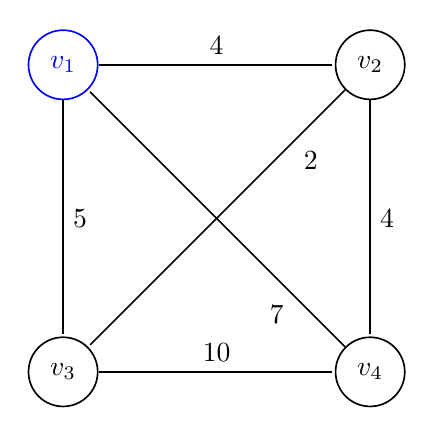
\begin{tikzpicture}[
    > = , % arrow head style
    shorten > = 1pt, % don't touch arrow head to node
    auto,
    node distance = 3cm, % distance between nodes
    semithick % line style
    ]

    \tikzset{every state}=[
    draw = black,
    thick,
    fill = white,
    minimum size = 1mm
    ]
    \node[state,blue] (v1) {$v_1$};
    \node[state] (v2) [right=of v1] {$v_2$};
    \node[state] (v3) [below =of v1] {$v_3$};
    \node[state] (v4) [below =of v2] {$v_4$};
  
    \path[->] (v1) edge  node[]{4}(v2);
    \path[->] (v1) edge  node[]{5}(v3);
    \path[->] (v2) edge  node[pos=0.2,below right]{2} (v3);
    \path[->] (v3) edge  node[]{10}(v4);
    \path[->] (v2) edge  node[]{4}(v4);
    \path[->] (v4) edge  node[pos=0.2,below left]{7}(v1);
\end{tikzpicture}
\end{center}
\underline{Step 2:}\\\\
Edge $\{v_1, v_2\}$ is chosen because it has the least weight amongst all edges that $v_1$ is adjacent to. Therefore, move to $v_2$ and mark $v_2$ as visited.
\begin{center}
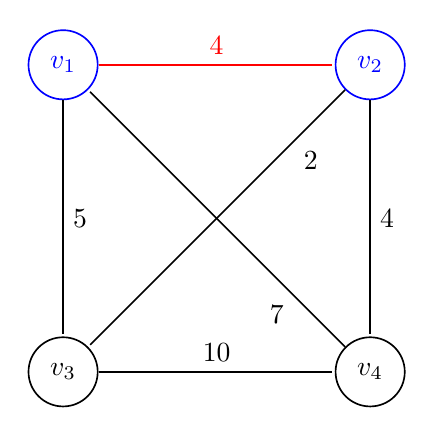
\begin{tikzpicture}[
    > = , % arrow head style
    shorten > = 1pt, % don't touch arrow head to node
    auto,
    node distance = 3cm, % distance between nodes
    semithick % line style
    ]

    \tikzset{every state}=[
    draw = black,
    thick,
    fill = white,
    minimum size = 1mm
    ]
    \node[state,blue] (v1) {$v_1$};
    \node[state, blue] (v2) [right=of v1] {$v_2$};
    \node[state] (v3) [below =of v1] {$v_3$};
    \node[state] (v4) [below =of v2] {$v_4$};
  
    \path[->] (v1) edge[red]  node[]{4}(v2);
    \path[->] (v1) edge  node[]{5}(v3);
    \path[->] (v2) edge  node[pos=0.2,below right]{2} (v3);
    \path[->] (v3) edge  node[]{10}(v4);
    \path[->] (v2) edge  node[]{4}(v4);
    \path[->] (v4) edge  node[pos=0.2,below left]{7}(v1);
\end{tikzpicture}
\end{center}
\underline{Step 3:}\\\\
Since not all vertices are visited, steps 1 and 2 above are repeated and thus, edge $\{v_2, v_3\}$ is chosen. Therefore, move to vertex $v_3$ and mark $v_3$ as visited.
\begin{center}
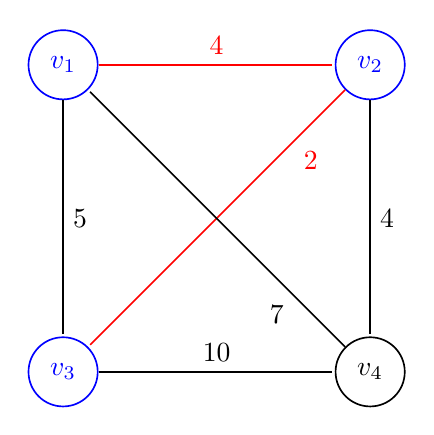
\begin{tikzpicture}[
    > = , % arrow head style
    shorten > = 1pt, % don't touch arrow head to node
    auto,
    node distance = 3cm, % distance between nodes
    semithick % line style
    ]

    \tikzset{every state}=[
    draw = black,
    thick,
    fill = white,
    minimum size = 1mm
    ]
    \node[state,blue] (v1) {$v_1$};
    \node[state,blue] (v2) [right=of v1] {$v_2$};
    \node[state,blue] (v3) [below =of v1] {$v_3$};
    \node[state] (v4) [below =of v2] {$v_4$};
  
    \path[->] (v1) edge[red]  node[]{4}(v2);
    \path[->] (v1) edge  node[]{5}(v3);
    \path[->] (v2) edge[red]  node[pos=0.2,below right]{2} (v3);
    \path[->] (v3) edge  node[]{10}(v4);
    \path[->] (v2) edge  node[]{4}(v4);
    \path[->] (v4) edge  node[pos=0.2,below left]{7}(v1);
\end{tikzpicture}
\end{center}
\underline{Step 4:}\\\\
Since not all vertices are visited, steps 1 and 2 above are repeated and thus, edge $\{v_3, v_4\}$ is chosen. Therefore, move to vertex $v_4$ and mark $v_4$ as visited.
\begin{center}
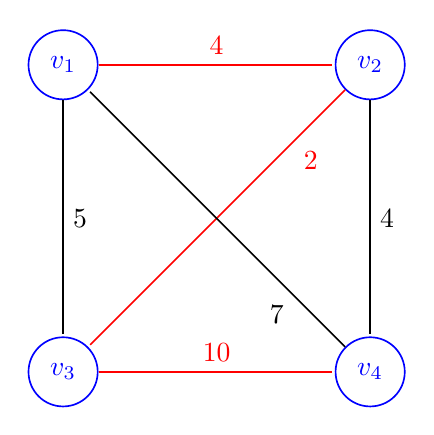
\begin{tikzpicture}[
    > = , % arrow head style
    shorten > = 1pt, % don't touch arrow head to node
    auto,
    node distance = 3cm, % distance between nodes
    semithick % line style
    ]

    \tikzset{every state}=[
    draw = black,
    thick,
    fill = white,
    minimum size = 1mm
    ]
    \node[state,blue] (v1) {$v_1$};
    \node[state,blue] (v2) [right=of v1] {$v_2$};
    \node[state,blue] (v3) [below =of v1] {$v_3$};
    \node[state,blue] (v4) [below =of v2] {$v_4$};
  
    \path[->] (v1) edge[red]  node[]{4}(v2);
    \path[->] (v1) edge  node[]{5}(v3);
    \path[->] (v2) edge[red]  node[pos=0.2,below right]{2} (v3);
    \path[->] (v3) edge[red]  node[]{10}(v4);
    \path[->] (v2) edge  node[]{4}(v4);
    \path[->] (v4) edge  node[pos=0.2,below left]{7}(v1);
\end{tikzpicture}
\end{center}
\underline{Step 5:}\\\\
Since all vertices are visited, the NNA moves to the starting vertex.
\begin{center}
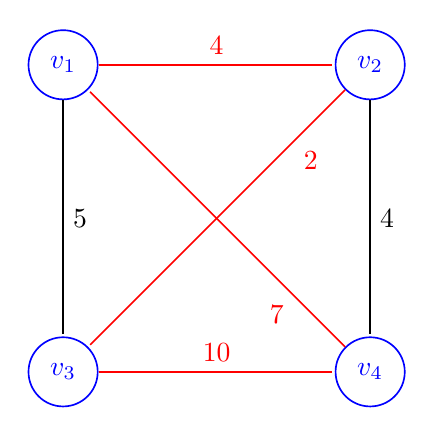
\begin{tikzpicture}[
    > = , % arrow head style
    shorten > = 1pt, % don't touch arrow head to node
    auto,
    node distance = 3cm, % distance between nodes
    semithick % line style
    ]

    \tikzset{every state}=[
    draw = black,
    thick,
    fill = white,
    minimum size = 1mm
    ]
    \node[state,blue] (v1) {$v_1$};
    \node[state,blue] (v2) [right=of v1] {$v_2$};
    \node[state,blue] (v3) [below =of v1] {$v_3$};
    \node[state,blue] (v4) [below =of v2] {$v_4$};
  
    \path[->] (v1) edge[red]  node[]{4}(v2);
    \path[->] (v1) edge  node[]{5}(v3);
    \path[->] (v2) edge[red]  node[pos=0.2,below right]{2} (v3);
    \path[->] (v3) edge[red]  node[]{10}(v4);
    \path[->] (v2) edge  node[]{4}(v4);
    \path[->] (v4) edge[red]  node[pos=0.2,below left]{7}(v1);
\end{tikzpicture}
\end{center}
Finally, the NNA returns the Hamiltonian cycle $v_1$, $v_2$, $v_3$, $v_4$, $v_1$ of weight 23.
\end{example}
It is important to note that in Example \ref{example_nna_explanation}, the minimum weight Hamiltonian cycle was not found. In fact, according to Example \ref{example_2.1}, the solution for the TSP given $G$ is the Hamiltonian cycle $v_1$, $v_3$, $v_2$, $v_4$, $v_1$ of weight 18. Note that the NNA would have found the optimal solution if it had started from vertex $v_2$. Since the approximate solution value does not differ a lot from the optimal value, this example seems to indicate that the NNA returns good approximations. However, this is not the case because, there could be instances where the NNA returns very bad approximations. The following example shows when the NNA can give bad approximations.
\begin{example}
\label{nna_fail}
\normalfont{Let} $M \in \mathbb{Z}^+$. Consider the graph $G$ below:
\begin{center}
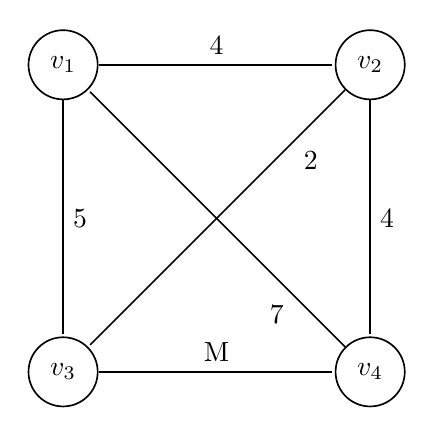
\begin{tikzpicture}[
    > = , % arrow head style
    shorten > = 1pt, % don't touch arrow head to node
    auto,
    node distance = 3cm, % distance between nodes
    semithick % line style
    ]

    \tikzset{every state}=[
    draw = black,
    thick,
    fill = white,
    minimum size = 1mm
    ]
    \node[state] (v1) {$v_1$};
    \node[state] (v2) [right=of v1] {$v_2$};
    \node[state] (v3) [below =of v1] {$v_3$};
    \node[state] (v4) [below =of v2] {$v_4$};
  
    \path[->] (v1) edge[]  node[]{4}(v2);
    \path[->] (v1) edge  node[]{5}(v3);
    \path[->] (v2) edge[]  node[pos=0.2,below right]{2} (v3);
    \path[->] (v3) edge[]  node[]{M}(v4);
    \path[->] (v2) edge  node[]{4}(v4);
    \path[->] (v4) edge[]  node[pos=0.2,below left]{7}(v1);
\end{tikzpicture}
\end{center}
Assuming that $M$ is a very large number, the minimum weight Hamiltonian cycle of $G$ is $v_2, v_3, v_1, v_4, v_2$ of weight 18. This minimum weight Hamiltonian cycle is found if the NNA starts from vertex $v_2$. Now, suppose that the NNA starts from vertex $v_1$. Then, NNA returns the Hamiltonian cycle $v_1$, $v_2$, $v_3$, $v_4$, $v_1$ of weight $M + 13$. This means that, since $M$ is a very large number, the NNA would return an approximate result that differs a lot in weight compared to the optimal solution. Therefore, in this case, the NNA returns a very bad approximation.
\end{example}
It can be concluded from Example \ref{nna_fail} that the quality of the result returned by the NNA depends heavily on which vertex the algorithm starts with, especially when the weights differ a lot. As seen in Example \ref{nna_fail}, this happens when the edge with a very large weight has to be used in order to complete the Hamiltonian cycle, or when all other vertices have been visited. In fact in Example \ref{nna_fail}, edge $\{v_3, v_4\}$ has to be used because, $current\_vertex$ was equal to $v_3$ but only $v_4$ was unvisited.\\\\
Since the NNA is an approximation algorithm, it is natural to ask what is it's approximation ratio. It can be deduced from Theorem \ref{no_approx_tsp} that, it is known that the NNA does not have a constant approximation ratio unless P=NP. In addition to this, By Theorem 1 in \cite{chekuri_im_2011}, unless P=NP, the approximation ratio of the NNA is not known in general. However, Rosenkrantz, Stearns and Lewis \cite{Rosenkrantz}, proved that, the NNA applied to an instance $G$ of the Metric-TSP has an approximation ratio that is logarithmic in the number of vertices in $G$. In what follows, a lemma will be proved. This will help in proving that the approximation ratio of the NNA applied to an instance $G$ of the Metric-TSP, is logarithmic in the number of vertices in $G$. Note that Lemma \ref{to_proove_bound} was constructed using ideas from \cite{Rosenkrantz}.
\begin{lemma}
\label{to_proove_bound}
Let G(V,E,f) be a complete weighted graph on $n$ vertices, and $W^\star$ be the optimal value of the Metric-TSP defined on G. Suppose that there exists a mapping g : V $\mapsto$ $\real^+$ such that, for all v $\in$ V, g(v) = $l_v$ and that the following  two conditions hold:
\begin{itemize}
\item $f(\{u, v\})$ $\geq$ min( $l_u$, $l_v$) for all $u$,$v$ $\in$ $V$
\item $l_u$ $\leq$ $\frac{1}{2}W^\star$ for all u $\in$ V
\end{itemize}
Then $\sum_{u \in V} l_u \leq \frac{1}{2}(\lceil log_2 n \rceil + 1)W^\star$. {\normalfont{\cite{Rosenkrantz}}}
\end{lemma}
\begin{proof}
Let $G(V,E,f)$ be a complete weighted graph on $n$ vertices, satisfying all the conditions in the Theorem statement. Suppose that $V=\{i | 1 \leq i \leq n\}$ and that, for all $i$, $j$ $\in$ V, if $i$ $\leq$ $j$ then $l_i$ $\geq$ $l_j$. Clearly, this just re-names and re-orders the vertices, hence, the generality of the proof is not effected.
\begin{claim}
\label{claim1}
$W^\star$ $\geq$ 2 $\sum_{i = k+1}^{min(2k, n)} l_i$, for all 1 $\leq$ $k$ $\leq$ n, where $k$ $\in$ $\mathbb{N}$.
\end{claim}
Let $H(V^\prime,E^\prime,f)$ be the complete weighted subgraph of $G$, such that, $V^\prime$ = $\{i | 1 \leq i \leq min(2k, n)\}$. Let $T$ be a sequence of vertices representing a Hamiltonian cycle in $H$, such that, the vertices are ordered as they would appear in a minimum weight Hamiltonian cycle of $G$. Let $C(V^\prime, E^{\prime\prime}, f)$ be the Cycle graph obtained from $T$ with weight $T^\star$. By the triangle inequality, for all $\{i, j\}$ $\in$ $E^{\prime\prime}$, $f(\{i, j\})$ is less than or equal to the weight of the path from $i$ to $j$ in a minimum weight Hamiltonian cycle of $G$. This holds because, the vertices in $T$ appear in the same order as in the minimum weight Hamiltonian cycle. Therefore, $T^\star$ $\leq$ $W^\star$. Now, by Definition \ref{weightofasubgraph}, $T^\star$ =  $\sum_{\{i, j\} \in E^{\prime\prime}} f(\{i, j\})$. Therefore, by the first bullet point in Lemma \ref{to_proove_bound},  $T^\star$ = $\sum_{\{i, j\} \in E^{\prime\prime}} f(\{i, j\})$ $\geq$  $\sum_{\{i, j\} \in E^{\prime\prime}} min(l_i, l_j)$. For each $i$ $\in$ [$min(2k, n)$], let $\alpha_i$ be the number of edges $\{i, j\}$ $\in$ $E^{\prime\prime}$, such that, $i > j$ ( i.e $l_i$ = $min(l_i, l_j)$). Then, $\sum_{\{i, j\} \in E^{\prime\prime}} min(l_i, l_j)$ = $\sum_{i \in E^\prime} \alpha_il_i$\\
$\implies$ $T^\star$ $\geq$ $\sum_{i \in E^\prime} \alpha_i l_i$ = $\sum_{i =1}^{min(2k, n)} \alpha_i l_i$.\\ Now, for all $i$ $\in$ [$min(2k, n)$], $\alpha_i$ $\leq$ 2. This is true because, every vertex $v_i$ is incident to exactly two edges of $C$. In addition to this, $\alpha_1$ + .. + $\alpha_{min(2k, n)}$ = $\abs{E^{\prime\prime}}$, because, for all $\{i,j\}$ $\in$ $E^{\prime\prime}$, either $ i \geq j$ or $j > i$. Therefore, either $\alpha_i$ or $\alpha_j$ is incremented by one. Another observation is that, $k$ is at least half of the number of vertices in $C$. This is true because of the following. Suppose that, $min(2k, n)$ = 2k. Then, by the construction of $C$ and $H$, $C$ contains $2k$ vertices. Hence, $k$ must be half of the number of vertices in $C$. Now, suppose that $min(2k, n)$ = $n$. Then, by the construction of $C$ and $H$, $C$ contains $n$ vertices. Now, $n$ $\leq$ $2k$, hence, $k$ must be at least half of the number of vertices in $C$. Therefore, from both cases, it can be deduced that $k$ is at least half of the number of vertices in $C$.
\begin{claim}
\label{claim2}
$\sum_{i =1}^{min(2k, n)} \alpha_i l_i$ $\geq$ 2 $\sum_{i = k + 1}^{min(2k, n)} l_i$.
\end{claim}
Since $k$ is at least half the number of vertices in $C$, and each $l_i$ is positive, 2 $\sum_{i = k + 1}^{min(2k, n)} l_i$ has the largest value when $k$ = $\frac{1}{2} min(2k, n)$. Therefore, if Claim \ref{claim2} can be proved for $k$ = $\frac{1}{2} min(2k, n)$, then Claim \ref{claim2} can be proved for all possible $k$. Let $k$ = $\frac{1}{2} min(2k, n)$ and $\alpha_i$ = 2 for all $i$ $\in$ [$k+1,min(2k, n)$]. Then, $\alpha_{k+1}$ + ... + $\alpha_{min(2k, n)}$ = 2($min(2k, n)$ - $k$) = 2($min(2k, n)$ -  $\frac{1}{2} min(2k, n)$ ) =  $min(2k, n)$ = number of edges in $C$. Therefore, since $\alpha_1$ + .. + $\alpha_{min(2k, n)}$ = $\abs{E^{\prime\prime}}$, then, $\alpha_i$ = 0 for all $i$ $\in$ [$k$]. Therefore, $\sum_{i =1}^{min(2k, n)} \alpha_i l_i$ = $\sum_{i = k + 1}^{min(2k, n)}2 l_i$ = 2 $\sum_{i = k + 1}^{min(2k, n)} l_i$. Therefore $\sum_{i =1}^{min(2k, n)} \alpha_i l_i$ $\geq$ 2 $\sum_{i = k + 1}^{min(2k, n)} l_i$, and hence, Claim \ref{claim2} is proved.\\\\
Now, since $W^\star$ $\geq$ $T^\star$ $\geq$ $\sum_{i =1}^{min(2k, n)} \alpha_i l_i$. Then, by Claim \ref{claim2}, $W^\star$  $\geq$ 2 $\sum_{i = k + 1}^{min(2k, n)} l_i$, and hence Claim \ref{claim1} is proved aswell.\\\\
By Claim \ref{claim1},  $W^\star$  $\geq$ 2 $\sum_{i = k + 1}^{min(2k, n)} l_i$. \\Hence,  $\sum_{j = 0}^{\lceil log_2 n \rceil - 1} W^\star$  $\geq$ $\sum_{j = 0}^{\lceil log_2 n \rceil -1} 2 \sum_{i = k + 1}^{min(2k, n)} l_i$. Letting $k$ = $2^{j}$,\\$\sum_{j = 0}^{\lceil log_2 n \rceil - 1} W^\star$  $\geq$ $\sum_{j = 0}^{\lceil log_2 n \rceil -1} 2 \sum_{i = 2^j + 1}^{min(2^{j+1}, n)} l_i$. \\$\implies$ $\lceil log_2 n \rceil$ $W^\star$  $\geq$ 2 $\sum_{i = 2}^{n} l_i$. Now, bullet point number two in Lemma \ref{to_proove_bound} implies that, $W^\star$ $\geq$ 2$l_1$. \\$\implies$ $\lceil log_2 n \rceil$ $W^\star$  $\geq$ 2 $\sum_{i = 1}^{n} l_i$.\\$\implies$  $\frac{1}{2}$ ($\lceil log_2 n \rceil$ + 1) $W^\star$  $\geq$ $\sum_{i = 1}^{n} l_i$ = $\sum_{u \in V} l_u$.
\end{proof}
Having proved Lemma \ref{to_proove_bound}, it is now time to prove that, when applied to an instance $G$ of the Metric-TSP, the NNA has an approximation ratio that depends logarithmically on the number of vertices in $G$. Note that the proof of Theorem \ref{log_bound_thrm} was constructed using ideas from \cite{Rosenkrantz}.
\begin{theorem}
\label{log_bound_thrm}
Suppose that $G(V,E,f)$ is an instance of the Metric-TSP. Let $W^\star$ be the optimal value of $G$, and apply the NNA on $G$. Suppose that $W$ is the value of the approximation returned by the NNA. Then, $\frac{W}{W^\star}$ $\leq$ $\frac{1}{2}(\lceil log_2 n \rceil + 1)$. {\normalfont\cite{Rosenkrantz}}
\end{theorem}
\begin{proof}
Define $G(V,E,f)$, $W^\star$, and $W$ as stated in Theorem \ref{log_bound_thrm}, and apply Algorithm \ref{nna_alg} to $G$. Let $g$ : $V$ $\mapsto$ $\real^+$ be the mapping defined by $g(v)$ = $f(\{v,u\})$, where $u$ is the vertex chosen by the NNA when $current\_vertex = v$. For all $v$ $\in$ $V$, let $l_v$ = $g(v)$. It will be shown that $g$ satisfies the two conditions of Lemma \ref{to_proove_bound}.\\\\
\textbf{Condition 1} :  $f(\{u, v\})$ $\geq$ min( $l_u$, $l_v$) for all $u$,$v$ $\in$ $V$\\\\
Let $u$, $v$ $\in$ $V$. Suppose that $u$ was set as visited by the NNA before $v$. Then, since $G$ is complete, $\{u, v\}$ was a candidate edge for the NNA when $current\_vertex$ was equal to $u$. Therefore, $f(\{u, v\})$ is greater than or equal to the weight of the edge selected when $current\_vertex$ was equal to $u$. Note that the weight of the selected edge is $l_u$. Therefore, $f(\{u, v\})$ $\geq$ $l_u$ (*). Using the same argument, if $v$ was set as visited by the NNA before $u$, then, $f(\{v, u\})$ = $f(\{u, v\})$ $\geq$ $l_v$ (**). Now, since the NNA must visit all veritices, either $u$ is visited before $v$ or vice-versa. As a result, one of (*) or (**) must hold. Hence, $f(\{u, v\})$ $\geq$ min($l_u$, $l_v$). Therefore, since $u$ and $v$ are arbitrary, Condition 1 holds.\\\\
\textbf{Condition 2} :  $l_u$ $\leq$ $\frac{1}{2}W^\star$ for all u $\in$ V\\\\
Let  $u$, $v$ $\in$ V such that, $l_u$ = $f(\{u, v\})$. Let $h$ be a minimum weight Hamiltonian cycle in $G$. Since $h$ is spanning a spanning subgraph, both $u$ and $v$ are in $h$. Therefore, $h$ can be expressed as the disjoint union of two paths joining $u$ and $v$. One of the paths can be obtain by starting from vertex $u$ and traversing through $h$ clockwise until finding $v$. The other path can be obtained by starting from vertex $u$ and traversing through $h$ anti-clockwise until finding $v$. Let these paths be $p_1$ and $p_2$ respectively. By the triangle inequality, the weight of $p_1$ and the weight of $p_2$ are both greater than or equal to $f(\{u,v\})$ in $G$. Therefore, summing both inequalities, 2$l_u$ = $2f(\{u,v\})$ $\leq$ weight of $p_1$ + weight of $p_2$ = weight of $h$ = $W^\star$. As a result, $l_u$ $\leq$ $\frac{1}{2}W^\star$. Therefore, since $u$ is arbitrary, Condition 2 holds.\\\\Now, for all $v$ in $V$, $l_v$ is the weight of the edge chosen by the NNA when $current\_vertex = v$. Therefore, $\sum_{u \in V} l_u $ =  $W$. Using Lemma \ref{to_proove_bound}, $W$ = $\sum_{u \in V} l_u $ $\leq$ $\frac{1}{2}$ ($\lceil log_2 n \rceil$ + 1) $W^\star$.\\ $\implies$ $W$ $\leq$ $\frac{1}{2}$ ($\lceil log_2 n \rceil$ + 1) $W^\star$\\ $\implies$ $\frac{W}{W^\star}$ $\leq$ $\frac{1}{2}$ ($\lceil log_2 n \rceil$ + 1).
\end{proof}
The implication of Theorem \ref{log_bound_thrm} is that when applying the NNA on an instance $G$ of the Metric-TSP, the quality of the approximation depends on the number of vertices in $G$. This is true because of the following. As the number of vertices increases, the approximation ratio increases logarithmically. Therefore, for very large $n$, $\frac{1}{2}(\lceil log_2 n \rceil + 1)$ may become very large that it may allow bad approximations to be returned by the NNA. These bad approximation would be returned because, their value would still be less than $\frac{1}{2}(\lceil log_2 n \rceil + 1)$ $\times$ optimal value. One way of solving this problem is to try and deduce whether the NNA can have a constant approximation ratio when applied to the Metric-TSP. This would solve the problem because, as the number of vertices increases, the quality of the approximation cannot worsen more than some fixed bound. Unfortunately, Rosenkrantz, Stearns and Lewis \cite{Rosenkrantz}, proved that there is an instance $G$ of the Metric-TSP such that, when the NNA is applied to $G$, it has an approximation ratio that is strictly bounded below by a logarithmic function of the number of vertices in $G$. This means that in general, the NNA cannot have a constant approximation ratio when applied to the Metric-TSP. This fact is stated in Theorem \ref{no_proof} below without proof because, the proof is too long.
\begin{theorem}
\label{no_proof}
For all m $>$ 3, m $\in$ $\mathbb{N}$, there is an instance $G(V,E,f)$ of the Metric-TSP such that, $\abs{V}$ = $2^m - 1$ and $\frac{W}{W^\star}$ $>$ $\frac{1}{3}$($log_2 (n+1))$ $+$ $\frac{4}{9}$, where $W$ is the optimal value of $G$, and $W^\star$ is the value of the approximation returned by the NNA when it is applied to $G$.{\normalfont{\cite{Rosenkrantz}}}
\end{theorem}
Theorem \ref{log_bound_thrm} and \ref{no_proof} imply that in general, the NNA cannot have a constant approximation ratio when applied to the Metric-TSP. However, this does not mean that the Metric-TSP cannot be approximated using an approximation algorithm that has a constant approximation ratio. In fact, an approximation algorithm that is known to have a constant approximation ratio when applied to the Metric-TSP is the Twice Around the Minimum Spanning Tree Approximation Algorithm. The Twice Around the Minimum Spanning Tree Approximation Algorithm will be presented in the next subsection.    
\subsubsection{Twice Around the Minimum Spanning Tree Approximation Algorithm}
\label{TAMSA_SECTION}
Similarly to the NNA, the Twice Around the Minimum Spanning Tree Algorithm (TAMSA) is an algorithm that can find near-optimal solutions to the TSP \cite{cormen_leiserson_rivest_stein}. The TAMSA computes an approximate solution to the TSP by using two other algorithms. In what follows, these two algorithms will be briefly described without delving into any specific details related to their implementation.\\\\
The first algorithm used by the TAMSA is Prim's algorithm. Prim's algorithm takes a connected weighted graph $G(V,E,f)$ and an arbitrary starting vertex $r$ $\in$ $V$ as inputs, and returns a minimum weight spanning tree $T(V^\prime,E^\prime,f)$ of $G$. Prim's algorithm computes $T$ in the following way. The algorithm initially starts with empty $V^\prime$ and empty $E^\prime$. Then, the algorithm proceeds by adding $r$ to $V^\prime$. Afterwards, the algorithm adds to $E^\prime$, the edge of least-weight connecting a vertex $v^\prime$ in $V^\prime$ to a vertex $v$ $\notin$ $V^\prime$. Following this, $v$ is added to $V^\prime$. The whole procedure is then repeated until all vertices in $V$ are added to $V^\prime$. \cite{harris_hirst_mossinghoff_2008}\\\\
An important question that must be answered is whether the procedure described in the previous paragraph does return a minimum weight spanning tree. Typically, one needs to show that the mathematical structure returned by Prim's algorithm is that of a spanning tree, whose weight is the least possible among all spanning trees of the input graph. Note that, the answer to this question is vital for algorithms that use Prim's algorithm to produce a minimum weight spanning tree. In fact, if Prim's algorithm does not return a minimum weight spanning tree, the algorithms that use Prim's algorithm need to use another algorithm to compute a minimum weight spanning tree. The next two theorems confirm that given an arbitrary connected weighted graph $G$ together with an arbitrary starting vertex $r$ as input, Prim's algorithm always returns a minimum weight spanning tree of $G$. Theorem \ref{correctness1} was constructed using ideas from \cite{prim's_algorithm}.
\begin{theorem}
\label{correctness1}
Prim's algorithm always returns a spanning tree {\normalfont{\cite{prim's_algorithm}}}.
\end{theorem}
\begin{proof}
Let $G(V,E,f)$ be a connected weighted graph, and $T(V^\prime,E^\prime,f)$ be the graph returned by Prim's algorithm when given $G$ and an arbitrary vertex $s$ $\in$ $V$ as input. Note that $s$ is the starting vertex for Prim's algorithm. To show that $T$ is a spanning tree, it must be shown that $T$ is a connected spanning subgraph of $G$ with no cycles. Note that $T$ is a subgraph of $G$ because, Prim's algorithm constructs $T$ using vertices and edges that belong to $G$.\\\\
Suppose that $T$ does not span $G$. Then, there exists a non-empty set of vertices $X$ $\subseteq$ $V$ such that, $X$ $\cap$ $V^\prime$ = $\emptyset$. Let $x$ $\in$ $X$. Then, $x$ $\notin$ $V^\prime$ and hence, there are no edges in $E$ of the form $\{v,x\}$ where $v$ $\in$ $V^\prime$, otherwise, Prim's algorithm would have chosen the edge and added $x$ to $V^\prime$. Now, since $G$ is connected, there exists a path $P$ in $G$ joining $s$ to $x$. In addition to this, $s$ $\in$ $V^\prime$ and $x$ $\in$ $X$. Hence, $P$ must contain an edge of the form $\{v, x\}$, where $v$ $\in$ $V^\prime$. This means that $E$ contains an edge of the form $\{v, x\}$, where $v$ $\in$ $V^\prime$. Contradiction. Therefore, $T$ must be a spanning subgraph of $G$.\\\\
To show that $T$ is connected, it must be shown that any two distinct vertices in $V^\prime$ are connected by a path. Let $u$, $v$ $\in$ $V^\prime$ such that $u$ $\neq$ $v$. Now, before Prim's algorithm adds $u$ to $V^\prime$, it connects it with a vertex $u_k$ which is already in $V^\prime$. But before $u_k$ was added to $V^\prime$, Prim's algorithm must have connected $u_k$ to a vertex $u_{k-1}$ that is already in $V^\prime$. Repeat this argument until reaching a vertex $z$, which is not connected to another vertex from a previous iteration of Prim's algorithm. Note that a vertex $z$ exists because, since there are a finite number of vertices in $V$, there are a finite number of vertices in $V^\prime$ that could have been chosen before $u$. From the description of Prim's algorithm above, this argument terminates when $z$ = $s$. This is true because, $s$ is the only vertex in $V$ which was not connected to another vertex in $V^\prime$ prior to being added to $V^\prime$. Now, suppose that $k$ vertices were added to $V^\prime$ before $u$. Then, $s= u_1, u_2, ..., u_k, u_{k+1} = u$ must be a path in $T$ joining $s$ to $u$ because, $\{u_i, u_{i+1}\}$ $\in$ $E^\prime$ for all $i$ $\in$ [$k$]. Now, the same argument can be repeated for $v$ and hence, $s$ and $v$ must also be connected by a path $P^\prime$. Therefore, since both $u$ and $v$ connect to the same vertex $s$ via a path, one can start from vertex $u$/$v$, travel to $s$ using $P$/$P^\prime$, and travel to $v$/$u$ using $P^\prime$/$P$. Therefore, $u$ and $v$ must be connected by a path. Hence, $T$ must be a connected spanning subgraph of $G$.\\\\
Suppose that $T$ contains a cycle $C$. Let $\{c_1, c_2\}$ be the last edge of $C$ that was added by Prim's algorithm to $E^\prime$ (hence the edge that caused the cycle to be created). WLOG, suppose that $c_1$ was added to $V^\prime$ by Prim's algorithm before $c_2$. Then, since Prim's algorithm adds an edge between a vertex in $V^\prime$ and a vertex not in $V^\prime$, it must be that $c_2$ is not in $V^\prime$ before $\{c_1, c_2\}$ is added to $E^\prime$. Hence, before $\{c_1, c_2\}$ is added to $E^\prime$, there are no paths in $T$ joining $c_1$ to $c_2$. This means that, no cycle is created when adding $\{c_1, c_2\}$ to $E^\prime$ because, $c_1$ would be connected to $c_2$ by exactly one path (the path $c_1, c_2$). Contradiction, since $\{c_1, c_2\}$ is the edge that caused the cycle to be created. Therefore, $T$ must be a connected spanning sub graph of $G$ without cycles, hence, by Definition \ref{spanning tree}, $T$ is a spanning tree of $G$.
\end{proof}
Theorem \ref{correctness1} confirms that Prim's algorithm returns a spanning tree. Now, it must be shown that the spanning tree returned by Prim's algorithm has the least possible weight among all spanning trees of $G$. Theorem \ref{correctness2} was constructed using ideas from \cite{prim's_algorithm}.
\begin{theorem}
Prim's algorithm always returns a minimum weight spanning tree {\normalfont{\cite{prim's_algorithm}}}.
\label{correctness2}
\end{theorem}
\begin{proof}
Let $G(V,E,f)$ be a connected weighted graph, and $T(V^\prime,E^\prime,f)$ be the spanning tree returned by Prim's algorithm when given $G$ and an arbitrary vertex $s$ $\in$ $V$ as inputs. Note that $s$ is the starting vertex for Prim's algorithm. Let $T^\star(V^\star,E^\star,f)$ be a minimum weight spanning tree of $G$. If $T$ = $T^\star$, the theorem holds.\\\\
Suppose that $T$ $\neq$ $T^\star$. Then,  $E^\prime$ $\setminus$ $E^\star$ $\neq$ $\emptyset$. Let $e = \{v_1, v_2\}$ $\in$  $E^\prime$ $\setminus$ $E^\star$. Let $S$ $\subset$ $V^\prime$ be the set of vertices in $V^\prime$ just before Prim's algorithm adds the edge $\{v_1, v_2\}$ to $E^\prime$. Although $e$ $\notin$ $E^\star$, there is a path $P$ joining $v_1$ to $v_2$ in $T^\star$, because, $T^\star$ is a spanning tree. Now, by construction of $S$, $v_1$ $\in$ $S$ and $v_2$ $\notin$ $S$. Hence, P is a sequence of vertices beginning with vertices in $S$, and ending with vertices which are not in $S$. Therefore, there exists some edge $e^\prime = \{x,y\}$ $\in$ $E^\star$ such that $x$ $\in$ $S$ and $y$ $\notin$ $S$. Now, in the iteration of Prim's algorithm when $V^\prime$ = $S$, both $e$ and $e^\prime$ connect a vertex which is in $V^\prime$ to a vertex which is not in $v^\prime$. Hence, both $e$ and $e^\prime$ are eligible to be chosen by Prim's algorithm at this stage. However, it is known that $e$ is chosen instead of $e^\prime$. This means that, $e$ is an edge of lesser weight than $e^\prime$. Now, if the edge $e^\prime$ is removed from $E^\star$ and replaced with the edge $e$, one gets a path $P^{\prime\prime}$ in $T^\star$ joining $x$ to $y$. Hence, ($T^\star$ $\setminus$ $P$) $\cup$ $P^{\prime\prime}$ would still remain a spanning tree. Let $T^\sim$ be the spanning tree ($T^\star$ $\setminus$ $P$) $\cup$ $P^{\prime\prime}$. Then, $T^\sim$ differs from $T^\star$ exactly in the edges $e$ and $e^\prime$, where, $f(e)$ $\geq$ $f(e^\prime)$. This means that, $T^\sim$ has weight at most that of $T^\star$. Now, since $T^\star$ is a minimum spanning tree, it must be a spanning tree of least weight. Hence, $f(T^\sim)$ = $f(T^\star)$. Therefore, if this procedure is repeated for every edge in $E^\prime$ $\setminus$ $E^\star$, $T^\star$ would be converted into a spanning tree $W^\prime = T$, where $f(T) = f(W^\prime) = f(T^\star)$. Therefore, $T$ must be a minimum weight spanning tree. Note that this holds because, the procedure can be repeated only for a finite number of times. This is true because, since $G$ is a finite graph, $|E^\prime$ $\setminus$ $E^\star|$ is a finite number.
\end{proof}
What follows is an example that demonstrates how Prim's algorithm constructs a minimum weight spanning tree from a connected weighted graph.
\begin{example}
\label{example_prim}
\normalfont{Consider} the graph $G$ in Example \ref{example4}, and the brief description of Prim's algorithm given in this subsection. Let $T(V^\prime,E^\prime)$ be the graph with an empty set of vertices, and an empty set of edges. Assuming that the starting vertex is $v_1$, Prim's algorithm starts by adding $v_1$ to $V^\prime$. Hence $T$ is now the following graph:
\begin{center}
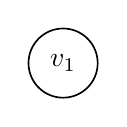
\begin{tikzpicture}[
    > = , % arrow head style
    shorten > = 1pt, % don't touch arrow head to node
    auto,
    node distance = 3cm, % distance between nodes
    semithick % line style
    ]

    \tikzset{every state}=[
    draw = black,
    thick,
    fill = white,
    minimum size = 1mm
    ]
    \node[state] (v1) {$v_1$};
\end{tikzpicture}
\end{center}
The algorithm now proceeds by adding the edge of least weight from $E$ to $E^\prime$, which connects a vertex $v^\prime$ $\in$ $V^\prime$ to a vertex $v$ $\notin$ $V^\prime$. Also, $v$ is added to $V^\prime$. In this example, these properties are satisfied by the edge $\{v_1, v_2\}$, hence, $T$ is the following graph.
\begin{center}
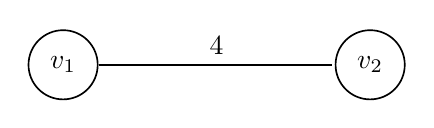
\begin{tikzpicture}[
    > = , % arrow head style
    shorten > = 1pt, % don't touch arrow head to node
    auto,
    node distance = 3cm, % distance between nodes
    semithick % line style
    ]

    \tikzset{every state}=[
    draw = black,
    thick,
    fill = white,
    minimum size = 1mm
    ]
    \node[state] (v1) {$v_1$};
    \node[state] (v2) [right=of v1] {$v_2$};
  
    \path[->] (v1) edge[]  node[]{4}(v2);
\end{tikzpicture}
\end{center}
Since not all vertices in $V$ have been added to $V^\prime$, the same procedure is repeated. Hence, the edge $\{v_2, v_3\}$ is chosen because, it is the edge of least weight connecting a vertex in $V^\prime$ to a vertex not in $V^\prime$. Therefore, $T$ is the following graph
\begin{center}
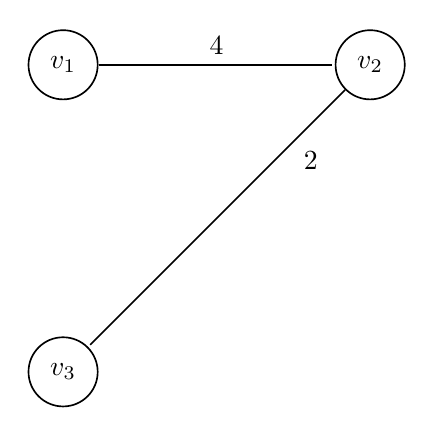
\begin{tikzpicture}[
    > = , % arrow head style
    shorten > = 1pt, % don't touch arrow head to node
    auto,
    node distance = 3cm, % distance between nodes
    semithick % line style
    ]

    \tikzset{every state}=[
    draw = black,
    thick,
    fill = white,
    minimum size = 1mm
    ]
    \node[state] (v1) {$v_1$};
    \node[state] (v2) [right=of v1] {$v_2$};
    \node[state] (v3) [below =of v1] {$v_3$};
  
    \path[->] (v1) edge[]  node[]{4}(v2);
    \path[->] (v2) edge[]  node[pos=0.2,below right]{2} (v3);
\end{tikzpicture}
\end{center}
Again, since not all vertices in $V$ have been added to $V^\prime$, the same procedure is repeated. In this case, $\{v_2, v_4\}$ is the edge of least weight connecting a vertex in $V^\prime$ to a vertex not in $V^\prime$. Therefore, $T$ is the following graph.
\begin{center}
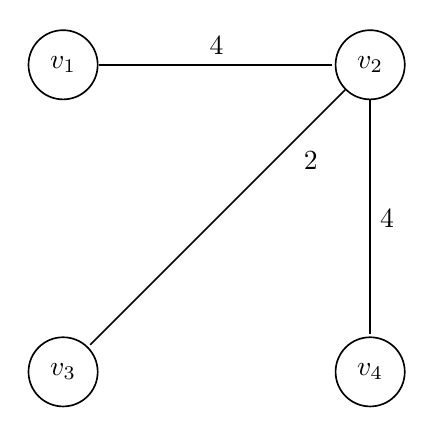
\begin{tikzpicture}[
    > = , % arrow head style
    shorten > = 1pt, % don't touch arrow head to node
    auto,
    node distance = 3cm, % distance between nodes
    semithick % line style
    ]

    \tikzset{every state}=[
    draw = black,
    thick,
    fill = white,
    minimum size = 1mm
    ]
    \node[state] (v1) {$v_1$};
    \node[state] (v2) [right=of v1] {$v_2$};
    \node[state] (v3) [below =of v1] {$v_3$};
    \node[state] (v4) [below =of v2] {$v_4$};
  
    \path[->] (v1) edge[]  node[]{4}(v2);
    \path[->] (v2) edge[]  node[pos=0.2,below right]{2} (v3);
    \path[->] (v2) edge  node[]{4}(v4);
\end{tikzpicture}
\end{center}
Since all vertices in $V$ have been added to $V^\prime$, the algorithm now terminates by returning $T$.
\end{example}
The second algorithm used by the TAMSA is the preorder tree walk algorithm, more commonly known as the depth first traversal tree algorithm. Given a tree $T(V,E,f)$ and an arbitrary starting vertex $r$ $\in$ $V$ as inputs, the preorder tree walk algorithm returns a walk $S$ of $T$ containing all vertices in $V$, where the vertices are ordered according to how they were visited while performing the walk. The preorder tree walk algorithm computes a walk $S$ in the following way. At the start of the algorithm, $S$ is empty. Then, starting from $r$, the algorithm marks $r$ as visited and adds $r$ to $S$. Following this, the algorithm recursively calls itself on all unvisited neighbors of $r$. The entire procedure is repeated until all vertices in $V$ are added to $S$. Note that in this dissertation, the execution of the preorder tree walk algorithm on an arbitrary tree will be termed as a preorder walk. For example, a preorder walk of the tree in Figure \ref{tree_example} below, results in the vertex sequence $v_1, v_2, v_3, v_4, v_5, v_9, v_6, v_7, v_8$. \cite{cormen_leiserson_rivest_stein}
\begin{center}
\begin{figure}[h]
\centering
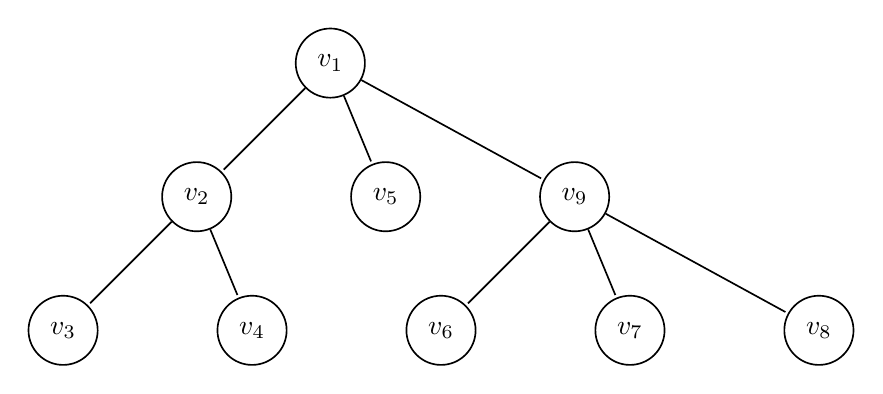
\begin{tikzpicture}[
    > = , % arrow head style
    shorten > = 1pt, % don't touch arrow head to node
    auto,
    node distance = 1.5cm, % distance between nodes
    semithick, % line style
    ]

    \tikzset{every state}=[
    draw = black,
    thick,
    fill = white,
    minimum size = 1mm
    ]
    \node[state] (v1) {$v_1$};
    \node[state] (v2) [below left=of v1] {$v_2$};
    \node[state] (v5) [right=of v2] {$v_5$};
    \node[state] (v9) [right =of v5] {$v_9$};
    \node[state] (v3) [below left =of v2]{$v_3$};
    \node[state] (v4) [right=of v3] {$v_4$};
    \node[state] (v6) [below left =of v9] {$v_6$};
    \node[state] (v7) [right=of v6] {$v_7$};
    \node[state] (v8) [right =of v7] {$v_8$};
  
    \path[->] (v1) edge[]  node[]{}(v2);
    \path[->] (v2) edge[]  node[]{} (v3);
    \path[->] (v2) edge  node[]{}(v4);
    \path[->] (v1) edge[]  node[]{}(v5);
    \path[->] (v1) edge[]  node[]{} (v9);
    \path[->] (v9) edge  node[]{}(v6);
    \path[->] (v9) edge  node[]{}(v7);
    \path[->] (v9) edge  node[]{}(v8);
\end{tikzpicture}
\caption{Tree example}
\label{tree_example}
\end{figure}
\end{center}
Having briefly described important algorithms that will be used by the TAMSA algorithm, it is now time to describe the TAMSA itself. The TAMSA takes an instance of the TSP as input, and returns a sequence of vertices representing a Hamiltonian cycle \cite{cormen_leiserson_rivest_stein}. The TAMSA algorithm can be described using the pseudocode below, which was adapted from \cite{cormen_leiserson_rivest_stein}.
\begin{algorithm}[H]
\begin{algorithmic}[1]
\State Choose an arbitrary vertex $r$ $\in$ V as starting vertex.
\State Starting from $r$, compute a minimum weight spanning tree $T$ of $G$ using Prim's algorithm.
\State Perform a preorder walk on T starting from $r$, and let $S$ be the walk returned by the preorder tree walk algorithm.
\State Add $r$ to $S$ as a final vertex and return S.
\caption{: TAMSA($G(V,E,f)$)}
\label{tamsa_alg}
\end{algorithmic}
\end{algorithm}
For the TAMSA to be a useful approximation algorithm for the TSP, it must guarantee that it will return a Hamiltonian cycle, and that the Hamiltonian cycle is computed in polynomial time. Let $G$ be an instance of the TSP, and let $T$ be the minimum weight spanning tree of $G$ returned by Prim's algorithm. By Theorem \ref{correctness2} and Theorem \ref{correctness1}, it is guaranteed that $T$ is a minimum weight spanning tree. Now, let $S$ be the sequence of vertices returned by a preorder walk on $T$. Since $T$ has no cycles, and visited vertices can never be visited again, a preorder tree walk of $T$ can never result into a walk with repetition of vertices. Hence, $S$ has no repetition of vertices. In addition to this, since $T$ is connected, the preorder tree walk algorithm terminates when all vertices of $G$ have been added to $S$. Therefore, $S$ must contain all vertices of $G$. Hence, $S$ must be a path containing all vertices of $G$. As a result, for $S$ to be a Hamiltonian cycle, the first vertex in $S$ must be repeated as a final vertex. This is done in line four of Algorithm \ref{tamsa_alg} above. Therefore, it can be concluded that $S$ must be a Hamiltonian cycle. The next step is to check that the Hamiltonian cycle is computed in polynomial time.\\\\
Given a TSP instance $G(V,E,f)$, the time complexity of the TAMSA is $O(|V|^2)$ \cite{cormen_leiserson_rivest_stein}. This is true because of the following. Consider Algorithm \ref{tamsa_alg} above. Clearly, the largest amount of work to be performed by the TAMSA is to compute a minimum weight spanning tree $T$ of $G$, and to compute a preorder tree walk of $T$. The preorder tree walk of $T$ takes $O(|V|)$ steps because, the preorder tree walk algorithm terminates when all the vertices in $G$ have been visited (this is true due to reasons mentioned in the previous paragraph). Hence, line number three in Algorithm \ref{tamsa_alg} takes $O(|V|)$ time. Now, according to Exercise 23.2-2 in \cite{cormen_leiserson_rivest_stein}, there is an implementation of Prim's algorithm that takes $O(|V^2|)$ time in order to compute a minimum weight spanning tree. Thus, the total time complexity of the TAMSA is $O(|V^2|)+ O(|V|) = O(|V^2|)$. However, in \cite{cormen_leiserson_rivest_stein} it is shown that the asymptotic time complexity of Prim's algorithm can be improved to $O(|E| log(|V|))$ by using a binary min-heap. This would mean that the time complexity of the TAMSA is no longer $O(|V^2|)$, but is $O(|E| log(|V|))$. As a result, the TAMSA would have a log-linear time complexity. Therefore, using Table \ref{tab:table1} in Section \ref{computational_theory}, and and the fact that the NNA has a quadratic time complexity (discussed in Section \ref{nna_section}), the TAMSA is more efficient asymptotically because, it has a smaller order of growth. Note that, the analysis of Prim's algorithm's time complexity is not given because, it requires theory about data structures such as Heaps to be presented, and this is out of the scope of this dissertation. What follows is an example which demonstrates how the TAMSA computes a Hamiltonian cycle.
\begin{example}
\label{tamsa_demonstration}
\normalfont{Consider} the graph $G$ in Example \ref{example4}, and Algorithm \ref{tamsa_alg} given in this subsection. Assume that randomly the TAMSA chooses vertex $v_1$ as starting vertex. From Example \ref{example_prim}, the minimum spanning tree $T$ returned by Prim's algorithm starting from vertex $v_1$ is the graph below.
\begin{center}
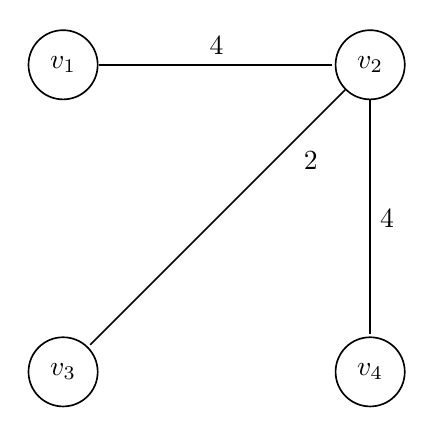
\begin{tikzpicture}[
    > = , % arrow head style
    shorten > = 1pt, % don't touch arrow head to node
    auto,
    node distance = 3cm, % distance between nodes
    semithick % line style
    ]

    \tikzset{every state}=[
    draw = black,
    thick,
    fill = white,
    minimum size = 1mm
    ]
    \node[state] (v1) {$v_1$};
    \node[state] (v2) [right=of v1] {$v_2$};
    \node[state] (v3) [below =of v1] {$v_3$};
    \node[state] (v4) [below =of v2] {$v_4$};
  
    \path[->] (v1) edge[]  node[]{4}(v2);
    \path[->] (v2) edge[]  node[pos=0.2,below right]{2} (v3);
    \path[->] (v2) edge  node[]{4}(v4);
\end{tikzpicture}
\end{center}
Now, according to bullet line number three in Algorithm \ref{tamsa_alg}, the TAMSA must perform a preorder tree walk on $T$ above. Consider the brief description of the preorder tree walk algorithm. A preorder walk of $T$ is computed in the following way. Note that, in the following demonstration, the blue vertices are the vertices that have already been visited by the preorder tree walk algorithm, and the black vertices are those vertices that have not yet been visited by the preorder tree walk algorithm.\\
The algorithm starts by visiting the starting vertex $v_1$ and adding it to $S$. Therefore, $S = v_1$.
\begin{center}
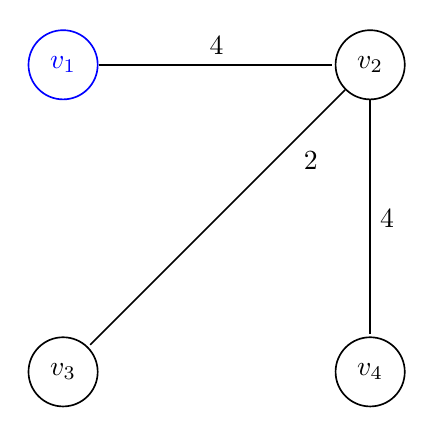
\begin{tikzpicture}[
    > = , % arrow head style
    shorten > = 1pt, % don't touch arrow head to node
    auto,
    node distance = 3cm, % distance between nodes
    semithick % line style
    ]

    \tikzset{every state}=[
    draw = black,
    thick,
    fill = white,
    minimum size = 1mm
    ]
    \node[state,blue] (v1) {$v_1$};
    \node[state] (v2) [right=of v1] {$v_2$};
    \node[state] (v3) [below =of v1] {$v_3$};
    \node[state] (v4) [below =of v2] {$v_4$};
  
    \path[->] (v1) edge[]  node[]{4}(v2);
    \path[->] (v2) edge[]  node[pos=0.2,below right]{2} (v3);
    \path[->] (v2) edge  node[]{4}(v4);
\end{tikzpicture}
\end{center}
Since not all vertices have been visited, the algorithm recursively calls itself on the unvisited neighbors of $v_1$, which in this case is only $v_2$. Hence, $v_2$ is visited and added to $S$. Therefore $S= v_1, v_2$.
\begin{center}
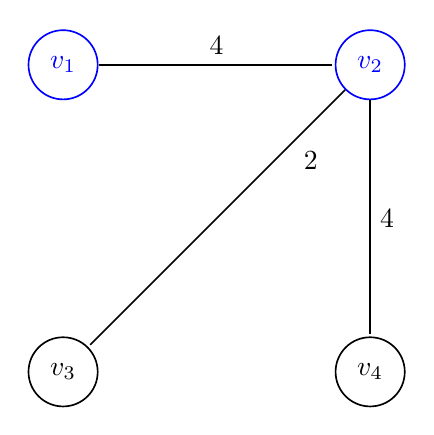
\begin{tikzpicture}[
    > = , % arrow head style
    shorten > = 1pt, % don't touch arrow head to node
    auto,
    node distance = 3cm, % distance between nodes
    semithick % line style
    ]

    \tikzset{every state}=[
    draw = black,
    thick,
    fill = white,
    minimum size = 1mm
    ]
    \node[state,blue] (v1) {$v_1$};
    \node[state,blue] (v2) [right=of v1] {$v_2$};
    \node[state] (v3) [below =of v1] {$v_3$};
    \node[state] (v4) [below =of v2] {$v_4$};
  
    \path[->] (v1) edge[]  node[]{4}(v2);
    \path[->] (v2) edge[]  node[pos=0.2,below right]{2} (v3);
    \path[->] (v2) edge  node[]{4}(v4);
\end{tikzpicture}
\end{center}
Since not all vertices have been visited, the algorithm recursively calls itself on the unvisited neighbors of $v_2$, which in this case are $v_3$ and $v_4$. Assuming that $v_3$ is visited before $v_4$, $v_3$ is marked as visited and added to $S$. Therefore $S= v_1, v_2, v_3$.
\begin{center}
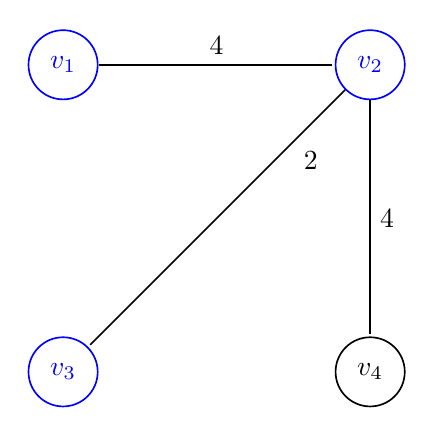
\begin{tikzpicture}[
    > = , % arrow head style
    shorten > = 1pt, % don't touch arrow head to node
    auto,
    node distance = 3cm, % distance between nodes
    semithick % line style
    ]

    \tikzset{every state}=[
    draw = black,
    thick,
    fill = white,
    minimum size = 1mm
    ]
    \node[state,blue] (v1) {$v_1$};
    \node[state,blue] (v2) [right=of v1] {$v_2$};
    \node[state,blue] (v3) [below =of v1] {$v_3$};
    \node[state] (v4) [below =of v2] {$v_4$};
  
    \path[->] (v1) edge[]  node[]{4}(v2);
    \path[->] (v2) edge[]  node[pos=0.2,below right]{2} (v3);
    \path[->] (v2) edge  node[]{4}(v4);
\end{tikzpicture}
\end{center}
Since not all vertices have been visited, and $v_3$ has no neighbors, the algorithm now visits another neighbor of $v_2$ which in this case is $v_4$. Hence $v_4$ is marked as visited and added to $S$. Therefore $S= v_1, v_2, v_3, v_4$.
\begin{center}
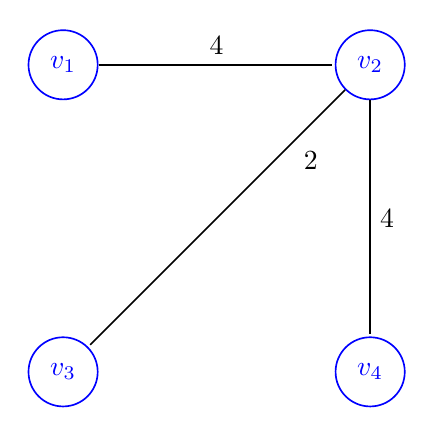
\begin{tikzpicture}[
    > = , % arrow head style
    shorten > = 1pt, % don't touch arrow head to node
    auto,
    node distance = 3cm, % distance between nodes
    semithick % line style
    ]

    \tikzset{every state}=[
    draw = black,
    thick,
    fill = white,
    minimum size = 1mm
    ]
    \node[state,blue] (v1) {$v_1$};
    \node[state,blue] (v2) [right=of v1] {$v_2$};
    \node[state,blue] (v3) [below =of v1] {$v_3$};
    \node[state,blue] (v4) [below =of v2] {$v_4$};
  
    \path[->] (v1) edge[]  node[]{4}(v2);
    \path[->] (v2) edge[]  node[pos=0.2,below right]{2} (v3);
    \path[->] (v2) edge  node[]{4}(v4);
\end{tikzpicture}
\end{center}
Since all vertices have been visited, the TAMSA adds $v_1$ to $S$ and returns it. Hence the TAMSA returns the Hamiltonian cycle $v_1, v_2, v_3, v_4, v_1$ of weight 23.
\end{example}
From Example \ref{tamsa_demonstration} and Example \ref{example_nna_explanation}, one can observe that the NNA and the TAMSA returned the same Hamiltonian cycle. Also similarly to the NNA, the TAMSA returns bad approximations for the graph presented in Example \ref{nna_fail}. This is true because of the following. Suppose that $G(V,E,f)$ is the graph in Example \ref{nna_fail}, and $v_1$ is the vertex chosen randomly by the TAMSA in line number one of Algorithm \ref{tamsa_alg} above, when given $G$ as input. The minimum weight spanning tree of $G$ is the same as the minimum weight spanning tree of the graph $G^\prime$ in Example \ref{example4}. This is true because, $G$ and $G^\prime$ differ only in the weight of the edge $\{v_3, v_4\}$, were this edge is not included in the minimum weight spanning tree of $G^\prime$. Hence, if $f(\{v_3, v_4\})$ is very large (greater than 10), and the other edge's weights remain the same, the edge $\{v_3, v_4\}$ will not be included in the minimum weight spanning tree of $G$ and hence, other edges will be used (which are identical to those of $G^\prime$). Since the minimum weight spanning tree of $G$ is the same as that of $G^\prime$, then by Example \ref{example_prim}, the TAMSA will return the Hamiltonian cycle $ H = v_1, v_2, v_3, v_4, v_1$ when given $G$ as input. Now, since $f(\{v_3, v_4\})$ is very large and $\{v_3, v_4\}$ is an edge in H, the weight of $H$ would be very large. As a result, the weight of $H$ would differ a lot from the optimal value. Note that, this problem would not happen if the preorder traversal is started from vertex $v_4$. In fact, the Hamiltonian cycle returned by the TAMSA would be $H = v_4, v_2, v_3, v_1, v_4$ (assuming $v_3$ is visited before $v_1$ when considering $v_2$), where the edge $\{v_3, v_4\}$ of weight $M$ is not in $H$. Therefore, from this paragraph it can be concluded that the quality of the approximation returned by the TAMSA depends on the starting vertex of the preorder walk.\\\\
Consider the TSP as defined in Definition \ref{TSP}. Similarly to the NNA, due to Theorem 1 in \cite{chekuri_im_2011}, the approximation ratio of the TAMSA when applied to the TSP is unknown unless P=NP. In addition to this, Theorem \ref{no_approx_tsp} guarantees that the TAMSA is not a constant approximation algorithm for the TSP, unless P=NP. Therefore, since it is not known whether P=NP, it is not known if the TAMSA is a constant approximation algorithm for the TSP. However, what is known is that the TAMSA is a 2-approximation algorithm for the Metric-TSP \cite{cormen_leiserson_rivest_stein}. This fact is proved in Theorem \ref{2_approx} below. Before proving Theorem \ref{2_approx}, the concept of a full walk will be explained because, it is going to be used in the proof.\\\\
Consider the preorder tree walk algorithm description provided in this subsection. Let $S$ be an arbitrary Hamiltonian cycle returned by the preorder tree walk algorithm. Suppose that the preorder tree walk algorithm is currently at a vertex $u$. According to the preorder tree walk algorithm description, the algorithm first marks $u$ as visited, adds $u$ to $S$, and then it recursively calls itself on all the unvisited neighbors $v_1, ..., v_k$ of $u$. From the preorder tree walk algorithm description it can be deduced that, the algorithm returns to $u$ when all unvisited vertices in the subgraph connected to the vertex $v_i$ for all $i$ $\in$ [$k$] are visited. In a preorder tree walk, when returning back to a vertex $v$, $v$ is not added again to $S$. To the contrary, in a full walk, when returning to a vertex $v$, $v$ is added again to $S$. Therefore, a full walk of a tree adds every vertex $v$ to $S$ whenever $v$ is first visited, and when $v$ is returned to after visiting one of the subgraphs connected to $v$ \cite{cormen_leiserson_rivest_stein}. In other words, a full walk is a preorder tree walk which lists a vertex every time it is visited. For example, a full walk of the tree in Figure \ref{tree_example} would result into the walk, $v_1, v_2, v_3, v_2, v_4, v_2, v_1, v_5, v_1, v_9, v_6, v_9, v_7, v_9, v_8, v_9, v_1$. Note that in a full walk, each edge is traversed exactly twice. This is true because, at each vertex $v$, the algorithm uses an edge $e$ to traverse to a neighbor $w$ of $v$, and uses the same edge $e$ when returning back to the vertex $v$, after all the unvisited vertices in the subgraph connected to $w$ are visited. Having described what a full walk is, it is now time to prove that the TAMSA is a 2-approximation algorithm when applied to Metric-TSP instances. Note that the proof for Theorem \ref{2_approx} below was constructed using ideas from \cite{cormen_leiserson_rivest_stein}.
\begin{theorem}
\label{2_approx}
The TAMSA is a 2-approximation algorithm for the Metric-TSP {\normalfont{\cite{cormen_leiserson_rivest_stein}}}.
\end{theorem}
\begin{proof}
Let $G(V,E,f)$ be an instance of the Metric-TSP, and $H^\star$ be a minimum weight Hamiltonian cycle of $G$. A spanning tree $T^\star$ can be obtained from $H^\star$ by deleting an edge from $H^\star$. This is true because, when deleting an edge from $H^\star$, no vertices of $G$ are deleted, hence, all vertices in $V$ would still be in $T^\star$. In addition to this, $T^\star$ has no cycles because, it contains less edges than vertices. As a result, by Definition \ref{spanning tree}, $T^\star$ is a spanning tree. Now, since every edge weight is positive, deleting an edge from a Hamiltonian cycle would result into a spanning tree of weight less than that of the Hamiltonian cycle. Furthermore, the weight of any spanning tree is greater than the weight of the minimum weight spanning tree. Hence, the weight of the minimum weight spanning tree gives a lower bound to the weight of the minimum weight Hamiltonian cycle. Therefore, letting $T$ be the minimum weight spanning tree of $G$, the following inequality holds:
\begin{equation}
\begin{split}
    \label{eq:1}
    f(T) \leq f(T^\star) \leq f(H^\star)\\
    \implies f(T) \leq f(H^\star)
 \end{split}
 \end{equation}
Now, let $W$ be a full walk of $T$. It was argued in this subsection that, a full walk of a tree $T^\prime$ uses an edge of $T^\prime$ exactly twice. Hence,
\begin{equation}
\begin{split}
    \label{eq:2}
    f(W) = 2f(T) \leq 2f(H^\star) \text{ (By Equation \ref{eq:1})}\\
    \implies f(W) \leq 2f(H^\star)
 \end{split}
 \end{equation}
However, $W$ is not a Hamiltonian cycle because it contains repetition of vertices. Now, since $G$ satisfies the triangle inequality, a path $P = u, v$ in $G$, has less weight than a path $P^\prime = u, c, v$ in $G$, for all $u, c, v$ $\in$ $V$. This means that, since a full walk returns to a vertex $u$ from a vertex $c$ and traverses to a vertex $v$, the full walk has a larger weight than that of traversing directly from $c$ to $v$ in $G$. Hence, by removing repetition of vertices in $W$, a sequence of vertices $H$ with the following properties is obtained. The first property is that $H$ is a Hamiltonian cycle. This is true because, $H$ contains every vertex exactly once (excluding the starting vertex of the cycle). The second property is that $H$ has a smaller weight than $W$. This is true because of the triangle inequality implications described in this paragraph. Due to the second property, the inequality below is satisfied.
\begin{equation}
\begin{split}
   \label{eq:3}
    f(H) \leq f(W)
 \end{split}
 \end{equation}
As described in this subsection, the difference between a full walk and a preorder walk is that in a preorder walk, vertices are not listed again when they are returned to. Hence, a preorder walk on a tree $T^\prime$ is equivalent to performing a full walk on a tree $T^\prime$ and deleting the repetition of vertices. This means that $H$ is the output of the preorder tree walk algorithm when given $T$ as input. Hence, $H$ is the Hamiltonian cycle outputted by the TAMSA. Therefore, from Equation \ref{eq:3} and Equation \ref{eq:2} it can be concluded that,
\begin{equation}
\begin{split}
   \label{eq:4}
    f(H) \leq f(W) \text{ (By Equation \ref{eq:3})}\\
    \implies f(H) \leq 2f(H^\star) \text{ (By Equation \ref{eq:2})}
 \end{split}
 \end{equation}
Hence, from Equation \ref{eq:4} it can be concluded that the value of the approximate solution returned by the TAMSA is within a constant factor of 2 from the optimal value. Hence, the TAMSA is a 2-approximation algorithm for the Metric-TSP.
\end{proof}
Therefore, Theorem \ref{2_approx} guarantees that the value of the approximation returned by the TAMSA when applied to the Metric-TSP, is never more than twice the optimal value, even for very large instance sizes. Recall that, this was not the case for the NNA. In fact, in Section \ref{nna_section} it was shown that, the approximation ratio for the NNA when applied to the Metric-TSP increases logarithmically with respect to the input size. That being said, it is stated in \cite{cormen_leiserson_rivest_stein} that although the TAMSA has a constant approximation ratio, it is not the best practical choice for the Metric-TSP. In fact, Christofides gave a 3/2-approximation algorithm for the Metric-TSP. However, this will not be discussed in this dissertation because, Christofides' algorithm requires presenting mathematical concepts which are out of the scope of this dissertation. These mathematical concepts are those of a minimum weight perfect matching.\\\\
In Section \ref{TAMSA_SECTION} and Section \ref{nna_section}, the aim was to present algorithms that approximate the TSP in polynomial time, and rigorously prove their approximation ratios when applied to a special case of the TSP (Metric-TSP). Although having approximation guarantees is important, it is sometimes better in practice in terms of accuracy of approximations, to design an algorithm that is guaranteed to find an optimal solution if given enough time to execute. Note that this statement will be justified when comparing the algorithm's performance in Chapter \ref{computational_section}. \\\\In the following section, two classes of algorithms called the heuristics and metaheuristics will be defined. Afterwards, an example of a metaheuristic called the Ant Colony Optimization Algorithm is going to be defined. After doing so, an example of an Ant Colony Optimization Algorithm called the Ant Colony System Algorithm will be given. After defining the Ant Colony System algorithm, the main aim is to prove that if given enough time to execute, the Ant Colony System applied to an arbitrary TSP instance $G$ will always find an optimal solution of $G$ (note that the time may be arbitrarily large).
\newpage
{\center{\section{The Ant Colony Optimization Algorithm}
\label{section_ACO}}}
As already discussed, the main aim of this Chapter is to present the Ant Colony Optimization (ACO) Algorithm, and describe how it can be applied to the TSP using the Ant Colony System approach. After doing this, the aim is to argue on why if given enough time to execute, the Ant Colony System algorithm always find an optimal solution of the TSP instance it is applied to. To understand the nature of the ACO algorithm better, it is important to define two classes of algorithms. One important class of algorithms is that of heuristics. Heuristics are algorithms that seek to obtain near-optimal solutions to a problem in polynomial time, without guaranteeing that an optimal solution will be found \cite{dorigo_stutzle_thomas_2004}. From what has been discussed so far, one can deduce that the TAMSA and the NNA are heuristic algorithms because, they both try to obtain near-optimal solutions to the TSP, without guaranteeing that the returned solution is an optimal one. The other important class of algorithms is that of metaheuristics.  A metaheuristic is a set of algorithmic notions that can be used to define heuristic methods for a wide variety of problems \cite{dorigo_stutzle_thomas_2004}. In other words this means that, a metaheuristic algorithm is a general framework that can be used to define different heuristics which may not solve the same problem. Note that a metaheuristic is different from a heuristic because, heuristic algorithms are specifically written to solve only one problem. For example, the NNA and the TAMSA can only approximate the TSP. Some examples of metaheuristic algorithms are Tabu Search, Simulated Annealing, Evolutionary Computing, and the ACO algorithm \cite{dorigo_stutzle_thomas_2004}. Note that for convenience, the terms `metaheuristic algorithm' and `algorithm' are used interchangeably in this chapter.\\\\
The ACO algorithm is a metaheuristic algorithm which was inspired from the behavior of ants in real ant colonies. Ants are capable of finding the shortest path from a food source to their nest and vice-versa without using any visual signals. Although ants do not use visual cues, it does not mean that they cannot communicate. In fact, ants deposit a chemical known as pheromone when they walk, and they probabilistically prefer to move into directions which are rich in pheromone. The trail of pheromone left behind by an ant while walking is called a pheromone trail. It is important to note that, an ant may still move in a direction which is not rich in pheromone, however, the probability of doing so is very small. The movement of ants in directions which are not rich in pheromone is important in real ant colonies because, it helps ants explore other ways of constructing a path from a food source to the nest which may result into a shorter path. \cite{dorigo_gambardella_1997}, \cite{dorigo_stutzle_thomas_2004}\\\\ 
The reason why ants are able to find short paths from a food source to their nest is because pheromone accumulates quicker on shorter paths. Pheromone accumulates quicker on shorter paths because of the following. Suppose that ants start to wander randomly to different directions in their environment starting from a food source. Obviously, ants that choose shorter paths to their nest will arrive much quicker than the ants that choose longer paths. This means that, on the way back to the food source, the ants that used the shorter paths will smell more pheromone on the shorter paths than on the longer paths because, the ants that choose the longer paths would have still not arrived at their nest (the pheromone trail is not yet constructed). In addition to this, pheromone evaporates gradually over time. Hence, the longer a path $P$ is, the more pheromone evaporation $P$ experiences until the ants using $P$ reach their destination. As a result, the ants would probabilistically prefer to move back to the food source using the shorter paths becaus, they simply would contain more pheromone. Over time, this would result into higher accumulation of pheromone on a shortest path, which would make the majority of the ants choose a shortest path in order to travel from their nest to a food source and vice-versa. What follows is an example which demonstrates at an abstract level how the ACO metaheuristic can be applied to the Shortest Path Problem defined in Example \ref{example decision/optimization}. \cite{dorigo_gambardella_1997}, \cite{dorigo_stutzle_thomas_2004}\\
\begin{example}
\label{explain_ACO}
\normalfont{Suppose} that the shortest path from vertex $v_1$ to vertex $v_4$ of the graph $G$ below must be found.
\begin{center}
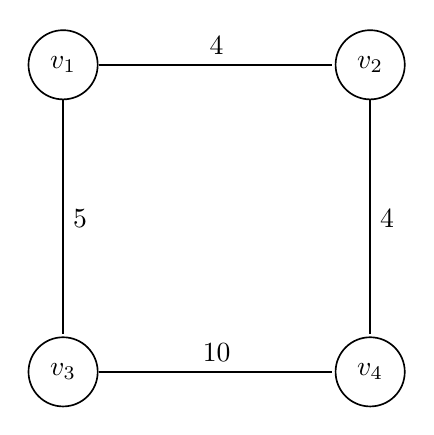
\begin{tikzpicture}[
    > = , % arrow head style
    shorten > = 1pt, % don't touch arrow head to node
    auto,
    node distance = 3cm, % distance between nodes
    semithick % line style
    ]

    \tikzset{every state}=[
    draw = black,
    thick,
    fill = white,
    minimum size = 1mm
    ]
    \node[state] (v1) {$v_1$};
    \node[state] (v2) [right=of v1] {$v_2$};
    \node[state] (v3) [below =of v1] {$v_3$};
    \node[state] (v4) [below =of v2] {$v_4$};
  
    \path[->] (v1) edge[]  node[]{4}(v2);
    \path[->] (v1) edge  node[]{5}(v3);
    \path[->] (v3) edge  node[]{10}(v4);
    \path[->] (v2) edge  node[]{4}(v4);
\end{tikzpicture}
\end{center}
Clearly, the ACO framework can be applied to the Shortest Path Problem on $G$ by letting the ant's environment be $G$, and the food source and the nest be $v_1$ and $v_4$ respectively. The ants would then find the shortest path due to the following. Since no ant has yet started to walk in it's environment, no pheromone has yet been deposited. Hence, for every ant starting at vertex $v_1$, $v_2$ and $v_3$ have the same probability of being chosen because no pheromone is yet deposited on the edges $\{v_1, v_2\}$, $\{v_1, v_3\}$. Hence, assuming that all ants at $v_1$ move at the same time, half of the ants probabilistically choose to move to $v_2$, and half of the ants probabilistically choose to move to $v_3$. Note that in the graphs below, the red and blue paths represent that different paths taken by the ants.
\begin{center}
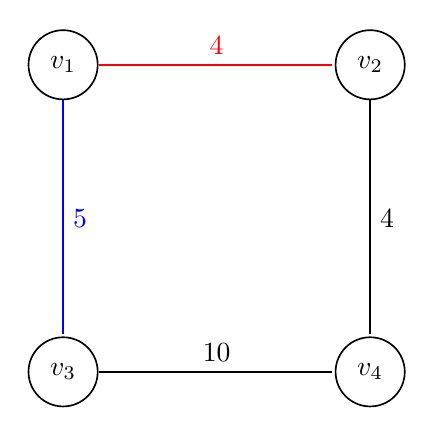
\begin{tikzpicture}[
    > = , % arrow head style
    shorten > = 1pt, % don't touch arrow head to node
    auto,
    node distance = 3cm, % distance between nodes
    semithick % line style
    ]

    \tikzset{every state}=[
    draw = black,
    thick,
    fill = white,
    minimum size = 1mm
    ]
    \node[state] (v1) {$v_1$};
    \node[state] (v2) [right=of v1] {$v_2$};
    \node[state] (v3) [below =of v1] {$v_3$};
    \node[state] (v4) [below =of v2] {$v_4$};
  
    \path[->] (v1) edge[red]  node[]{4}(v2);
    \path[->] (v1) edge[blue]  node[]{5}(v3);
    \path[->] (v3) edge  node[]{10}(v4);
    \path[->] (v2) edge  node[]{4}(v4);
\end{tikzpicture}
\end{center}
Suppose that a constraint is added such that each ant does not visit vertices that it has already visited. This can be easily done by assigning a list of vertices to each ant $k$ which contains the vertices that ant $k$ has already visited. As a result, the ants at $v_3$ and $v_2$ have only one vertex to move to because $v_1$ has already been visited. Therefore, all ants from $v_2$ and $v_3$ move to vertex $v_4$.
\begin{center}
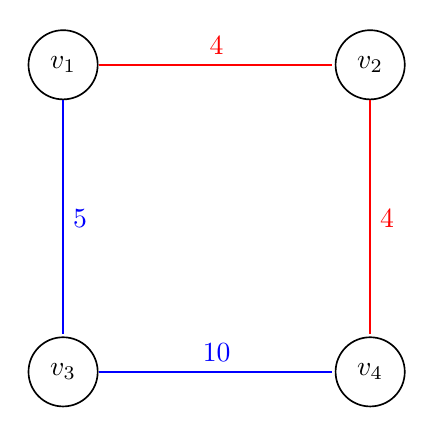
\begin{tikzpicture}[
    > = , % arrow head style
    shorten > = 1pt, % don't touch arrow head to node
    auto,
    node distance = 3cm, % distance between nodes
    semithick % line style
    ]

    \tikzset{every state}=[
    draw = black,
    thick,
    fill = white,
    minimum size = 1mm
    ]
    \node[state] (v1) {$v_1$};
    \node[state] (v2) [right=of v1] {$v_2$};
    \node[state] (v3) [below =of v1] {$v_3$};
    \node[state] (v4) [below =of v2] {$v_4$};
  
    \path[->] (v1) edge[red]  node[]{4}(v2);
    \path[->] (v1) edge[blue]  node[]{5}(v3);
    \path[->] (v3) edge[blue]  node[]{10}(v4);
    \path[->] (v2) edge[red]  node[]{4}(v4);
\end{tikzpicture}
\end{center}
Now, since the red path is shorter than the blue path, the ants following the red path arrive at vertex $v_4$ before the ants following the blue path. Hence, on the way back to vertex $v_1$, the red path has more pheromone than the blue path because, more pheromone is evaporated on the longer path until all ants arrive at $v_4$. Therefore, the majority of the ants at $v_4$ would probabilistically choose to travel to $v_1$ using the red path. As a result, the red path keeps on accumulating more pheromone than the blue path and eventually this would lead to a situation were almost all ants would choose the red path when traveling from $v_1$ to $v_4$ and vice-versa. To conclude, the ACO algorithm for the Shortest Path Problem given the instance $(G, v_1, v_4)$, can then return the best found path $P$ (in this case the red path) when either the majority of the ants are traveling through $P$, or, it can return $P$ after a maximum number of iterations are reached.  
\end{example}
Having described the basic idea behind the ACO metaheuristic, it is now time to describe the requirements the algorithm which implements the ACO framework must follow, in order to be successfully applied to the TSP. Let $G(V,E,f)$ be an instance of the TSP. As described in Example \ref{explain_ACO}, the ant's environment can be represented by $G$. In addition to this, since the goal of the TSP is to find a minimum weight Hamiltonian cycle, it does not matter which vertex represents the food source, and which vertex represents the nest because all vertices have to be visited. What is important is that when an ant starts traversing vertices in a graph, it doesn't move to vertices that it has already visited. This can be done as discussed in Example \ref{explain_ACO} above, by giving each ant a list of vertices called  the working memory, which is used to remember which vertices it has already visited. Note that although real ants do not posses a working memory, the working memory is vital for the artificial ants (ants in the algorithm) to compute a Hamiltonian cycle, otherwise, ants may produce walks of $G$ with repetition of vertices. Another important thing is that the artificial ants must keep the order of how the vertices are visited. This can be easily done by always adding a new vertex that an ant visits at the end of the working memory. In what follows, a specific type of ACO metaheuristic will be discussed in detail with specific reference to how it can be applied to the TSP. This metaheuristic algorithm is called the Ant Colony System (ACS) algorithm in literature. \cite{dorigo_gambardella_1997}, \cite{dorigo_stutzle_thomas_2004}\\\\
The ACS algorithm for the TSP can be described as follows. Suppose that $G(V,E,f)$ is a TSP instance. At the start of the algorithm, each ant is placed on a random vertex of $G$. At each time step, every ant $k$ is moved to a vertex of $G$ which is not in the working memory of ant $k$, and this is repeated until all vertices of $G$ are in the working memory of ant $k$. The new vertex that each ant must move to is determined using a probabilistic function. As discussed so far in this subsection, the ants must probabilistically prefer to move in directions with high pheromone. Hence, at each time step, the probabilistic function must be in such a way that every ant should probabilistically prefer to choose vertices, which are connected via edges to the vertex the ant is currently on, with high pheromone. However, since the TSP is based on finding shorter connections, then the length of the edges must also effect the direction the ants must move to. Therefore, the probabilistic function must be a function of both the pheromone accumulated on the edges, and of the length of the edges connecting the current vertex the ant is on with a candidate vertex, where, the higher the weight of an edge $e$  is, the less chance $e$ has of being chosen by an ant. Due to this probabilistic function, ants would probabilistically prefer to move to vertices that are connected by edges with high pheromone and which are close-by. \cite{dorigo_gambardella_1997}, \cite{dorigo_stutzle_thomas_2004}\\\\
Another important component of the ACS algorithm is local trail updating. Local trail updating is the reduction of pheromone on the edges chosen by an ant at each time step. The aim of local trail updating is to reduce the pheromone of an edge $e$, after it is chosen by an ant so that $e$ is less desirable for other ants. Local trail updating is important because, it increases the probability that ants explore other edges that were not visited by any other ant, and hence, lowers the probability that the ants generate the same sub-optimal solution repeatedly. It is important to note that, local trail updating was inspired from pheromone evaporation in real ant colonies. In what has been discussed so far, it was argued that pheromone accumulates quicker on shorter paths in real ant colonies. The ACS algorithm encourages this behavior by making the ants that produce the shorter Hamiltonian cycles deposit more pheromone on the edges constituting their Hamiltonian cycle at every iteration. As a result, there would be more pheromone present on edges that constitute the shorter Hamiltonian cycles. This procedure is called global trail updating. One way to go about global trail updating is to make the ant that produces the best Hamiltonian cycle since the first iteration of the algorithm, add more pheromone on the edges constituting it's Hamiltonian cycle. Note that the ant that produces the best Hamiltonian cycle since the first iteration will be referred to as the `global best ant', and it's Hamiltonian cycle will be referred to as the `global best Hamiltonian cycle'. Another way to go about global trail updating is to make the ant that produces the iteration's best Hamiltonian cycle deposit more pheromone on the edges constituting it's Hamiltonian cycle. Note that the ant which produces the iteration's best Hamiltonian cycle will be referred to as the `iteration's best ant'. According to \cite{dorigo_stutzle_thomas_2004}, the former is better than the latter empirically. Hence, in what remains, global trail updating is performed by the global best ant. \cite{dorigo_gambardella_1997}, \cite{dorigo_stutzle_thomas_2004} \\\\
It is important to note that there are different ACO algorithms that could have been applied to the TSP. The ACS algorithm was chosen because, it is one of the most empirically successful ACO algorithms in terms of accuracy of approximations \cite{dorigo_stutzle_thomas_2004}. It is important to note that later on in this chapter, other ACO algorithms will be briefly described, by discussing how they vary from the ACS algorithm. The discussion will now proceed by presenting the pseudocode of an algorithm (Algorithm \ref{ACO_ALG}) for the TSP that implements the ACS framework. In Algorithm \ref{ACO_ALG} below, $G(V,E,f)$ is an instance of the TSP, and $g$ is a probabilistic function with the properties described in the previous paragraphs. Also, $a.current\_vertex$ is the variable containing the vertex that ant $a$ is currently on. Note that Algorithm \ref{ACO_ALG} was constructed using ideas from \cite{dorigo_gambardella_1997}.
\begin{algorithm}[H]
\begin{algorithmic}[1]
\State $best\_ham\_cycle$ = ()
\State $best\_ham\_cycle.weight$ = $\infty$
\While{(!finished)}
          \State Place $m$ new ants on $m$ randomly selected vertices in $V$.
          \While{not all ants have completed a Hamiltonian cycle of $G$}
		\For {every ant $a$}
			\State move $a$ to vertex $v$ $\in$ $V$ chosen using the probabilistic function $g$.
			\State Perform local trail updating on the edge $\{a.current\_vertex, v\}$
		\EndFor
	\EndWhile
	\State $A$ = Iteration's best ant.
	\If{$best\_ham\_cycle.weight$ $\geq$ $A.Hamiltonian\_Cycle.weight$}
		\State $best\_ham\_cycle$ = $A.Hamiltonian\_Cycle$
	\EndIf
           \State Perform global pheromone update on the edges of $G$ constituting the Hamiltonian cycle $best\_ham\_cycle$
\EndWhile
\State Return $best\_ham\_cycle$
\caption{: ACS\_TSP($G(V,E,f)$)}
\label{ACO_ALG}
\end{algorithmic}
\end{algorithm}
For Algorithm \ref{ACO_ALG} to be implemented, there remains to define the probabilistic function $g$, the global trail updating formula, and the local trail updating formula. As stated in \cite{dorigo_gambardella_1997}, there are different ways how the probabilistic function and the global/local trail updating formulas can be defined. However, the ones suggested by Dorigo and Gambardella in \cite{dorigo_gambardella_1997} will be presented. Note that the probabilistic function, and the local/global trail updating formula will be presented in their general form (i.e. for the ACS algorithm applied to any problem). While presenting these formulas, it will be discussed how they can be applied to the TSP. Note that from this point onward, any definitions and terms that will be defined, will be used throughout the entire section. \\\\Let $G(V,E,f)$ be an instance of the TSP. An ant $k$ on vertex $r$ chooses the vertex $s$ to move to among those vertices which do not belong to its working memory $M_k$, by applying the probabilistic formula below.
\begin{equation}
  \label{eq:aco1}
  s=\begin{cases}
            \displaystyle{\argmax\limits_{u \notin M_k} \left\{[\tau(\{r,u\})].\left[\eta(\{r, u\})\right]^\beta \right\}} &\text{   if $q$ $\leq$ $q_0$}\\ 
             S &\text{ 	otherwise}
            \end{cases}
\end{equation}
where $\tau(\{r,u\})$ is the amount of pheromone on the edge $\{r,u\}$, $\eta(\{r,u\})$ is a problem specific function where for the TSP it was chosen to be the inverse of the weight of the edge $\{r,u\}$, $\beta$ is a parameter which weighs the importance of the pheromone level of an edge $\{r,u\}$ and the closeness of $u$ to $r$, 0 $\leq$ $q$ $\leq$ 1 is a random value chosen with uniform probability, 0 $\leq$ $q_0$ $\leq$ 1 is another parameter, and $S$ is a random variable which is selected according to the following probability distribution:
\begin{equation}
  \label{eq:aco2}
  p_k(\{r,s\})=\begin{cases}
             \displaystyle {\frac{[\tau(\{r,s\})].[\eta(\{r, s\})]^\beta}{\sum_{u \notin M_k} [\tau(\{r,u\})].[\eta(\{r, u\})]^\beta }} &\text{ if $s$ $\notin$ $M_k$}\\ 
             0 &\text{ 	otherwise}
            \end{cases}
\end{equation}
where $p_k(r,s)$ is the probability of ant $k$ on vertex $r$ to choose vertex $s$. \cite{dorigo_gambardella_1997}\\\\
The idea behind Formula \ref{eq:aco1} is the following. When an ant $k$ wants to move to a new vertex, it picks a random number $q$ in the interval [0,1], where each number in this interval has equal probability of being chosen. Then, if $q$ $\leq$ $q_0$, since $\eta$ was chosen to be the inverse of the weight of an edge, the edge with the largest amount of pheromone per edge weight is chosen. It is important to note that, the larger the amount of pheromone on an edge is, the more chance an edge has to be the maximum element in the argument list of Formula \ref{eq:aco1}. In addition to this, the smaller the weight of an edge is, the more chance an edge has to be the maximum element in the argument list of Formula \ref{eq:aco1}. Therefore, it can be concluded that the case $q$ $\leq$ $q_0$ makes an ant choose the edge with the largest amount of pheromone per edge weight. In other words, the case $q$ $\leq$ $q_0$ forces an ant to choose the edge which has been chosen by the majority of ants as required by the ACO metaheuristic. \cite{dorigo_gambardella_1997}, \cite{dorigo_stutzle_thomas_2004}\\\\
When $q$ is less than $q_0$, the ant randomly picks a vertex with probability defined by the probability distribution in Formula \ref{eq:aco2} above. The idea behind Formula \ref{eq:aco2} above is the following. If a vertex is already in the working memory of an ant, then it has no chance of being selected. Hence, it's probability is zero. This will ensure that ants will not produce a walk with repetition of vertices. If a vertex $s$ is not in the working memory of an ant $k$, the probability of ant $k$ on vertex $r$ to choose vertex $s$ depends on the amount of pheromone on the edge $\{r,s\}$ per edge weight of $\{r,s\}$, where, the larger this ratio is, the larger the probability of the vertex $s$ is to being chosen. Therefore, this equation makes an ant probabilistically prefer edges with large pheromone and small weight. However, unlike the case $q$ $\leq$ $q_0$ in Equation \ref{eq:aco1}, this does not mean that a vertex with a small probability cannot be chosen. This mimics the case when real ants move to directions which are not rich in pheromone. As discussed earlier, this is necessary in real ant colonies because it may help ants to find shorter paths from a food source to their nest. Similarly, the movement of artificial ants to vertices with low probability defined by Formula \ref{eq:aco2}, may help the algorithm find Hamiltonian cycles of lesser weight. \cite{dorigo_gambardella_1997}, \cite{dorigo_stutzle_thomas_2004}\\\\
Therefore, from the above two paragraphs it can be concluded that, an ant can either move to new vertices using experience gathered from previous ants with probability $q_0$ (using the largest amount of pheromone per edge weight), or it can perform a biased exploration towards edges of small weight but with high pheromone levels with probability $(1-q_0)$. As a result, the value of $q_0$ determines the amount of exploration that will be performed by the ACS algorithm. According to  \cite{dorigo_gambardella_1997}, the best value of $q_0$ was empirically found to be 0.9. From this observation one can deduce that, it is more important for the ACS to gather information from previous ants than exploring other edges in the TSP instance. \cite{dorigo_gambardella_1997}, \cite{dorigo_stutzle_thomas_2004}\\\\
The next formula that needs to be presented is the global trail updating formula. As discussed previously, the idea behind global trail updating is to reward edges which belong to shorter Hamiltonian cycles with more pheromone. It was also discussed that this will be achieved by forcing the global best ant to add more pheromone on the edges that belong to it's Hamiltonian cycle. The global trail updating formula can be seen in Formula \ref{eq:aco3} below, and it is the one presented in \cite{dorigo_stutzle_thomas_2004}. Therefore, the global best ant performs global trail updating on every edge $\{r,s\}$ forming part of it's solution, using the formula below:
\begin{equation}
  \label{eq:aco3}
  \tau(\{r,s\})=(1-p).\tau(\{r,s\})+ p.\Delta\tau(\{r,s\})
\end{equation}
where $\tau(\{r,s\})$ is the amount of pheromone on edge $\{r,s\}$, $p$ is the evaporation rate which mimics evaporation of pheromone in real ant colonies, and $\Delta\tau(\{r,s\})$ is a problem specific value which for the TSP is chosen to be the inverse of the weight of the global best Hamiltonian cycle.\\\\
From Formula \ref{eq:aco3} it can be deduced that, the shorter the global best Hamiltonian cycle is, the larger $\Delta\tau(\{r,s\})$ is, and hence, the more pheromone is added to the edges of the global best Hamiltonian cycle. As a result, this will accumulate more pheromone on the edges belonging to shorter Hamiltonian cycles, and thus make shorter Hamiltonian cycles more desirable for other ants. As already remarked, although it is desirable to have a lot of pheromone on the edges that form part of short Hamiltonian cycles, the ACS algorithm must not create a situation where an edge is always chosen by all ants. Otherwise, as previously discussed, the ants may not find shorter Hamiltonian cycles. As it can be seen in Formula \ref{eq:aco3}, this problem is solved by reducing some of the added pheromone by the aid of the evaporation rate $p$. As a result, $p$ is typically a value in the interval (0,1]. In fact, Dorigo and Gambardella \cite{dorigo_gambardella_1997}, found out empirically that the best value of $p$ is 0.1. \cite{dorigo_gambardella_1997}\\\\
For Algorithm \ref{ACO_ALG} to be implemented, there remains to present the local trail updating formula. The local trail updating formula that will be presented is the one suggested in \cite{dorigo_stutzle_thomas_2004}. Therefore, when an ant on vertex $r$ chooses vertex $s$, it modifies the pheromone on the edge $\{r,s\}$ using the local trail updating formula below.
\begin{equation}
  \label{eq:aco4}
  \tau(\{r,s\})=(1-\zeta).\tau(\{r,s\})+\zeta.\tau_0
\end{equation}
where $\tau_0$ is the value representing the amount of pheromone deposited on an edge when it is chosen by an ant, $\tau(\{r,s\})$ is the amount of pheromone on edge $\{r,s\}$, and 0 $<$ $\zeta$ $<$ 1 is the evaporation rate. It is important to note that $\tau_0$ and $\zeta$ are usually chosen in such a way that after the local trail updating formula is applied, the pheromone on the chosen edge is reduced. This is important because as discussed before, the aim of local trail updating is to avoid having all ants choosing the same edges. As a result, an experimentally good value for $\zeta$ was found to be 0.1, and an experimentally good value for $\tau_0$ was experimentally found to be $\displaystyle{\frac{1}{nC^{nn}}}$ where $n$ is the number of vertices in the TSP instance, and $C^{nn}$ is the length of the Hamiltonian cycle returned by the NNA. It is important to note that normally, the pheromone values of the edges at the start of the algorithm are initialized to the value of $\tau_0$. Another observation is that although $\zeta$ and $p$ both represent the evaporation rate, their values can be different. \cite{dorigo_gambardella_1997}, \cite{dorigo_stutzle_thomas_2004}\\\\
As already remarked, the ACO algorithm that was applied to the TSP in this section was the ACS algorithm. However, there are other ACO algorithms that could have been applied to the TSP. Two of these ACO algorithms are the Ant System (AS), and the Elitist Ant System (EAS). The main difference between the ACS, AS and EAS is how the pheromones on the edges are updated from one iteration to the next. For example in the AS, no pheromone update is carried out until all ants compute a solution of the problem they are applied to. In addition to this, after all ants compute their solution, every edge in the graph gets it's pheromone reduced. After all edges get their pheromone reduced, all ants add more pheromone on the edges they used. One can observe that this differs a lot from the ACS because, the AS performs pheromone evaporation on all edges in the graph. In addition to this, unlike the ACS, the AS does not perform global trail updating. The other ACO algorithm variant that was mentioned in this paragraph is the EAS. The EAS is an extension of the AS, where the only difference is that at each iteration, the global best ant adds more pheromone on the edges that constitute it's solution. Note that the AS and the EAS where only briefly described to show that there are other ACO algorithms that can be applied to any problem including the TSP. A detailed explanation on these ACO algorithms is given in \cite{dorigo_stutzle_thomas_2004}. \cite{dorigo_stutzle_thomas_2004}\\\\
Since ants are capable of finding a shortest path from a food source to their nest, it is now natural to ask whether the ACS algorithm is able to find a minimum weight Hamiltonian cycle if given enough time to execute, when applied to the TSP. More generally, if a problem $P$ can be solved by an ACO algorithm $A$, will $A$ eventually find an optimal solution of $P$? In literature, when an optimization algorithm (algorithm for an optimization problem) $A$ finds an optimal solution for a problem, $A$ is said to converge. It is important to note that, if an ACO algorithm $A$ converges, then $A$ can find the optimal solution of every problem that it can be applied to. Unfortunately, it is not easy to determine whether the ACO metaheuristic converges because, the brief history of the ACO metaheuristic is a history of experimental research \cite{dorigo_stutzle_thomas_2004}. In addition to this, the fact that the ACO metaheuristic can be applied to a wide variety of problems, makes theoretical analysis very difficult \cite{dorigo_stutzle_thomas_2004}. Due to these reasons, all of the convergence results about the ACO metaheuristic that are known of only apply to specific variants (ex. ACS) \cite{dorigo_stutzle_thomas_2004}.\\\\
As already hinted in the previous paragraph, the theoretical property of algorithms that will be analyzed in this project is that of convergence. In general, there are at least two types of convergence in the ACO framework. These are convergence in value, and convergence in solution. An optimization algorithm converges in value if it generates an optimal solution at least once. On the other hand, an optimization algorithm converges in solution if it reaches a state which repeatedly generates the same optimal solution. It is important to note that, although convergence in solution is stronger than convergence in value, in this chapter only convergence in value will be considered. The reason is that, in optimization, the algorithm solving the optimization problem will never find a better approximation value once an optimal solution is found. For example, in Algorithm \ref{ACO_ALG}, once the value of best\_ham\_cycle.weight becomes equal to the optimal value, it will never change again because, the optimal value is the smallest possible value. In what follows, an ACO algorithm variant called $ACO_{bs, \tau_{min}}$ will be defined, and it will be shown that the $ACO_{bs, \tau_{min}}$ algorithm converges in value if given enough time to execute. Afterwards, it will be shown that the proof of convergence of $ACO_{bs, \tau_{min}}$ applies also to the ACS. As a result, it can then be confirmed that, when applied to the TSP, the ACS will eventually converge to the weight of a minimum weight Hamiltonian cycle if given enough time to execute (i.e. when applied to the TSP,  if given enough time to execute, the ACS will always find an optimal solution at least once). \cite{dorigo_stutzle_thomas_2004}\\\\
In what has been discussed so far, it has always been assumed that the ants perform walks on the instance of the optimization problem that is inputted to the ACO algorithm implemented. For example in the ACS for the TSP, the ants perform walks directly on the TSP graph instance. However, this can only be done if the instance of the problem being consider is a graph instance. Optimization problems who's instances are not a graph require their instances to be transformed into graph instances. Otherwise if not, the ACO algorithm cannot be applied on that problem. Therefore, before defining the $ACO_{bs, \tau_{min}}$ algorithm, a number of concepts must first be formalized. Note that the terms/concepts that will be defined/formalized/generalized from this point onward will be used throughout in what follows. A minimization problem $P$ can be defined as a triple $(S, f, \Omega)$ where, $S$ is the set of all candidate solutions of $P$, $f$ : S $\mapsto$ $\real^+$ is called the cost function, and $\Omega$ is a set of constraints which defines the set of feasible candidate solutions $\widetilde{S}$ $\subseteq$ $S$. As a consequence of this definition, $s^\star$ $\in$ $\widetilde{S}$ is an optimal solution of $P$ if $f(s^\star)$ $\leq$ $f(s)$ for all $s$ $\in$ $S$. In general, $P$ can be mapped to a new problem $A$ which can be characterized in terms of a graph as follows. Let $C=\{c_1, c_2, ..., c_N\}$ be a set of components/vertices, where $N$ is the size of $C$, and let $X$ be the finite set of states the algorithm solving the problem $A$ can be in, defined in terms of all possible sequences $(c_i, c_j, ..., c_h, ...)$ over the elements of $C$, such that the length of every state is finite. Denote by $n$ the maximum possible length of an element $x$ in $X$. In addition to this, let $C$ and $S$ be in such a way that $S$ $\subseteq$ $X$. Also, let $\widetilde{X}$ $\subseteq$ X be a set of states of $A$ such that, if an element $x$ is in $\widetilde{X}$, then, $x$ can be transformed into an element $s$ which satisfies $\Omega$ by adding more components to $x$. As a result, $s$ $\in$ $\widetilde{S}$. In addition to this, let $S^\star$ be the set of all optimal solutions of $A$. As a result, $S^\star$ $\subseteq$ $\widetilde{X}$ and $S^\star$ $\subseteq$ $S$. Given the definitions in this paragraph, an ACO algorithm can then be applied to $A$ such that, the ants perform walks on the graph $G_c=(C,L,\mathrm{T})$, where $L$ is the set of edges that fully connects the components in $C$, and $\mathrm{T}$ is a matrix of pheromone trails, where $\tau_{ij}$=$\mathrm{T_{ij}}$ denotes the pheromone value of the edge $\{c_i, c_j\}$ in $G_c$. It is important to note that in this case, the graph $G_c$ will not posses the property of changing with respect to time. Hence, the problems that will be considered in this chapter are static with respect to time (static problems for short). Therefore, the convergence proofs that will be presented later on in this chapter only apply to static problems. Note that the TSP is a static problem because, the graph instance does not change during an algorithm's execution. Note that, what is important to take from these formalizations is that, if a minimization problem $P$ is to be solved using an ACO algorithm, then a graph $G_c$ must be constructed for the ants to solve $P$. \cite{dorigo_stutzle_thomas_2004}\\\\
To understand better the concepts formalized in the previous paragraph, these concepts are now going to be presented in the context of the TSP. The TSP can be represented formally as an optimization problem as follows. Given a TSP instance $G(V,E,g)$, $S$ can contain tuples of vertices in $G$, where repetition of vertices in the tuples is allowed. As a result, $S$ contains all possible walks in $G$. Since in the TSP, weights of walks must be optimized, the cost function $f$ is chosen to be $g$. The set of feasible candidate solutions $\widetilde{S}$ must contain the solutions which satisfy the problem's constraints. Hence, in the context of the TSP, the solutions in $\widetilde{S}$ must form a Hamiltonian cycle. As a result, the constraints in $\Omega$ must force $\widetilde{S}$ to contain only Hamiltonian cycles. Therefore, two constraints are only needed in $\Omega$. The first constraint in $\Omega$ is that every $s$ in $\widetilde{S}$ must be of the form $(v_1, v_2, ...,v_n, v_1)$, where apart from $v_1$, no other vertex is allowed to be repeated in $s$. The second constraint in $\Omega$ is that for every $s$ in $\widetilde{S}$, $s$ must contain all the vertices in $V$. The next term that needs to be defined is $S^\star$. In the context of the TSP, $S^\star$ is the set of all minimum weight Hamiltonian cycles in $G$. Now, since the TSP's instance are graphs, the ants can directly use $G$ to perform it's walks. As a result, $G_c$ = $G$, $C = V$ and $E=L$. What remains to be defined is $X$ and $\widetilde{X}$. In the context of the TSP, $X=S$ and $\widetilde{X}$ is the set of all elements in $X$ of the form $x$ = $(v_1, v_2, ..., v_n)$, such that if more vertices are added to $x$, $x$ is transformed into a Hamiltonian cycle.\\\\
Given the definitions and terms defined in the previous paragraphs, it is now time to define the $ACO_{bs, \tau_{min}}$ algorithm. The algorithm starts by initializing the pheromones in $\mathrm{T}$ to $\tau_0$ $>$ 0, where, $\tau_0$ is the same parameter as in Equation \ref{eq:aco4}. Secondly, each ant is placed on a vertex of the graph $G_c$, where the vertex is chosen according to problem the $ACO_{bs, \tau_{min}}$ algorithm is applied to (normally the starting vertices are chosen randomly with uniform probability). Thirdly, the ants are moved around $G_c$, and $\Omega$ is used to prevent infeasible solutions from being constructed. Afterwards, step 2 and step 3 are repeated for a number of iterations, where the terminating condition depends on the problem the $ACO_{bs, \tau_{min}}$ algorithm is applied to. Similarly to the ACS, there remains to describe the probabilistic function to be used by ants when choosing new components/vertices (vertices and components are used interchangeably) of $G_c$, and how the pheromones are updated at each iteration. Suppose that ant $k$ is currently on component $c_i$. Having constructed the solution $x_h= (v_1, v_2, ..., v_h = c_i)$, ant $k$ chooses the component $c_j$, according to the following probability distribution.
\begin{equation}
  \label{eq:gen1}
  P(v_{h+1}=c_j | x_h)\begin{cases}
             \displaystyle {\frac{\tau_{ij}^\alpha}{\sum_{\{c_i,c_l\} \in N_i^k}  \tau_{il}^\alpha}} &\text{if } \{c_i,c_j\} \in N_i^k\\ 
             0 &\text{ 	otherwise}
            \end{cases}
\end{equation}
where, $\{c_i,c_j\}$ $\in$ $N_i^k$ iff the solution $(v_1, v_2, ..., v_h = c_i, c_j)$ built by ant $k$ is an element of $\widetilde{X}$ (i.e. the solution built by ant $k$ forms part of a feasible solution), and $\alpha$ is a parameter in the interval $(0,\infty)$. As it can be seen from the probability distribution in Equation \ref{eq:gen1}, the ants in the $ACO_{bs, \tau_{min}}$ algorithm probabilistically prefer to move to feasible components of $G_c$ (the solution is still in $\widetilde{X}$ when the new component is chosen) connected by edges which are rich in pheromone, as required by every ACO algorithm. Note that, if an edge $\{c_i, c_j\}$ is not in $N_i^k$, then $c_j$ has no chance of being selected because, it's probability is zero. This had to be done because of the following. Suppose that an ant has constucted the solution $(v_1, v_2, ..., v_h = c_i)$. If $\{c_i, c_j\}$ is not in $N_i^k$, then the solution $(v_1, v_2, ..., v_h = c_i, c_j)$ is not $\widetilde{X}$, hence it invalidates $\Omega$. Therefore, $(v_1, v_2, ..., v_h = c_i, c_j)$ is not a feasible solution, and hence it should not be constructed. \cite{dorigo_stutzle_thomas_2004}\\\\
After defining the probabilistic function, there remains to describe how the pheromones in $\mathrm{T}$ should be updated from one iteration to the next. Once all the ants have completed a solution in $\widetilde{X}$, the values in $\mathrm{T}$ are decreased by a small factor 0 $<$ $p$ $\leq$ 1, where $p$ is the same parameter as in Equation \ref{eq:aco3} (the evaporation rate). In other words, the pheromone levels of all edges $\{c_i, c_j\}$ in $G_c$ are decreased by a small factor $p$ using the formula below:
\begin{equation}
  \label{eq:gen2}
  \tau_{ij}= (1-p)\tau_{ij}
\end{equation}
Let $s^{bs}$ be the global best solution of the $ACO_{bs, t_{min}}$ algorithm. After pheromone evaporation is performed, the pheromone value of the edges constructing $s^{bs}$ are increased by a value $q_f(s^{bs})$, where $q_f$ is defined by $q_f$ : $\widetilde{S}$ $\mapsto$ $\real^+$ such that, if $f(s_1)$ $>$ $f(s_2)$ then $q_f(s_1)$ $\leq$ $q_f(s_2)$ ($f$ is the minimization's problem cost function). In literature, $q_f$ is called a quality function, and the procedure of updating the pheromones of the edges constructing the global best solution is called global-best pheromone update. For example in the ACS, $q_f(s)$ = $\frac{1}{f(s)}$, where clearly, if  $f(s_1)$ $>$ $f(s_2)$ then $q_f(s_1)$ $\leq$ $q_f(s_2)$. Therefore, after Equation \ref{eq:gen2} is performed for every edge in $G_c$, the following equation is performed for every edge $\{c_i, c_j\}$ in $s^{bs}$: 
\begin{equation}
  \label{eq:gen3}
  \tau_{ij}= \tau_{ij} + q_f(s^{bs})
\end{equation}
An additional constraint is also put on the pheromones in $\mathrm{T}$. The constraint says that, the smallest entry of $\mathrm{T}$ cannot be less than some parameter $\tau_{min}$ $>$ 0. As a result, after Equations \ref{eq:gen2} and \ref{eq:gen3} are performed, the algorithm must check all the entries of $\mathrm{T}$, to verify that every entry in $\mathrm{T}$ is greater than $\tau_{min}$. If an entry $e$ in $\mathrm{T}$ is less than $\tau_{min}$, the algorithm must overwrite the value at entry $e$ to that of $\tau_{min}$. Therefore, for every edge $\{c_i, c_j\}$ in $G_c$, the $ACO_{bs, \tau_{min}}$ algorithm updates $\tau_{ij}$ using the following formula:
\begin{equation}
  \label{eq:gen4}
  \tau_{ij}= max\{\tau_{ij}, \tau_{min}\}
\end{equation}
To summarize, the pheromone update procedure that will be used in the $ACO_{bs, \tau_{min}}$ algorithm can be characterized by the following. Pheromone update is performed only after all ants compute a solution. After all ants compute their solutions, every edge in $G_c$ gets it's pheromone reduced by a factor $p$, which mimics pheromone evaporation in real ant colonies. After pheromone evaporation is carried out, global-best pheromone update is performed to reward solutions which are more feasible than others, with more pheromone. Finally, if any entry $e$ in $\mathrm{T}$ has value less than $\tau_{min}$, then $e$ is overwritten to $\tau_{min}$. In what follows it will be assumed that $\tau_{min}$ $<$ $q_f(s^\star)$, where $s^\star$ is the optimal solution of the problem the $ACO_{bs, \tau_{min}}$ algorithm is applied to. Note that this can be achieved by setting $\tau_0$ = $\frac{q_f(s^\prime)}{2}$, where $s^\prime$ is any solution in $\widetilde{S}$ ($\tau_{min}$ $\leq$ $\tau_0$ =  $\frac{q_f(s^\prime)}{2}$ $\leq$ $\frac{q_f(s^\star)}{2}$ $<$ $q_f(s^\star)$). \cite{dorigo_stutzle_thomas_2004}\\\\
After defining the $ACO_{bs, \tau_{min}}$ algorithm, it is now time to present two lemmas. These two lemmas will be used to show that the $ACO_{bs, \tau_{min}}$ algorithm converges in value to an optimal solution $s^\star$ of the static problem the algorithm is applied to. The first lemma states that the pheromone value of any edge in $G_c$ cannot exceed that of $\tau_{max}$ = $\frac{q_f(s^\star)}{p}$, even if the algorithm is executed for an infinite number of iterations. In what follows, all the concepts/terms defined in this chapter are assumed. In addition to these definitions, let $\theta$ denote an arbitrary iteration of the $ACO_{bs, \tau_{min}}$ algorithm, and $\tau_{ij}(\theta)$ denote the value of $\tau_{ij}$ at iteration $\theta$. Note that the proof of Lemma \ref{lemma1_aco} was constructed using ideas from \cite{dorigo_stutzle_thomas_2004}.
\begin{lemma}
\label{lemma1_aco}
 For any i, j $\in$ {\normalfont{[}}N{\normalfont{]}}, $\lim\limits_{\theta\to\infty}$ $\tau_{ij}(\theta)$ $\leq$ $\tau_{max}$ = $\frac{q_f(s^\star)}{p}$ {\normalfont{\cite{dorigo_stutzle_thomas_2004}}}.
\end{lemma}
\begin{proof}
Since $f(s^\star)$ $<$ $f(s)$ $\forall$ $s$ $\in$ $\widetilde{S}$ such that $s$ $\neq$ $s^\star$, then, by definition of $q_f$, $q_f(s^\star)$ $\geq$ $q_f(s)$ $\forall$ $s$ $\in$ $\widetilde{S}$, such that $s$ $\neq$ $s^\star$ (*).
\\\\ Now, from Equation \ref{eq:gen3} it can be deducated that, $q_f$ determines the amount of pheromone to be added to the edges constituting the global-best solution $s^{bs}$. In addition to this, edges which do not form part of $s^{bs}$ do not get more pheromone. Hence, (*) implies that the maximum amount of pheromone that can be added to any edge $\{c_i, c_j\}$ is $q_f(s^\star)$, and this is true for all iterations of the $ACO_{bs, \tau_{min}}$ algorithm. As a result, by Equations \ref{eq:gen2} and \ref{eq:gen3}, and the fact that $\tau_{min}$ $<$ $q_f(s^\star)$, the maximum amount of pheromone that can be present on any edge after one iteration is $(1-p)\tau_0 + q_f(s^\star)$, where $\tau_{ij}(0)$ = $\tau_0$ as already described. Similarly, the maximum amount of pheromone that an edge can have at iteration two is $(1-p)^2\tau_0 + (1-p)q_f(s^\star) + q_f(s^\star)$. Hence, in general, any edge in iteration $\theta$ can have a maximum pheromone value of $\tau_{ij}^{max}(\theta)$ =  $(1-p)^\theta\tau_0$ + $\sum_{i=1}^{\theta} (1-p)^{\theta-i}q_f(s^\star)$. Now, since $\tau_{ij}(\theta)$ $\leq$ $\tau_{ij}^{max}(\theta)$ for any $\theta$, then  $\lim\limits_{\theta\to\infty}$ $\tau_{ij}(\theta)$ $\leq$  $\lim\limits_{\theta\to\infty}$ $\tau_{ij}^{max}(\theta)$. In addition to this, $\tau_{ij}^{max}(\theta)$ = $(1-p)^\theta\tau_0$ + $\sum_{i=1}^{\theta} (1-p)^{\theta-i}q_f(s^\star)$ = $(1-p)^\theta\tau_0$ + $\sum_{i=0}^{\theta-1} (1-p)^{i}q_f(s^\star)$. Therefore, $\lim\limits_{\theta\to\infty}$ $\tau_{ij}^{max}(\theta)$ = $\lim\limits_{\theta\to\infty}$ $(1-p)^\theta\tau_0$ + $\lim\limits_{\theta\to\infty}$ $\sum_{i=0}^{\theta-1} (1-p)^{i}q_f(s^\star)$. Hence, $\lim\limits_{\theta\to\infty}$ $\tau_{ij}^{max}(\theta)$ = $\lim\limits_{\theta\to\infty}$ $\sum_{i=0}^{\infty} (1-p)^{i}q_f(s^\star)$ = $\frac{q_f(s^\star)}{p}$. Therefore,  $\lim\limits_{\theta\to\infty}$ $\tau_{ij}(\theta)$ $\leq$  $\lim\limits_{\theta\to\infty}$ $\tau_{ij}^{max}(\theta)$ = $\frac{q_f(s^\star)}{p}$, and hence, $\lim\limits_{\theta\to\infty}$ $\tau_{ij}(\theta)$ $\leq$ $\frac{q_f(s^\star)}{p}$ as required.
\end{proof}
The next lemma that will be proved states that, once an optimal solution $s^\star$ is found by the $ACO_{bs, \tau_{min}}$ algorithm, and the number of iterations $\theta$ become arbitrarily large, the pheromone values of all edges constituting $s^\star$ converge to $\tau_{max}$ defined in Lemma \ref{lemma1_aco}. In what follows, for all $i$, $j$ $\in$ [$N$] such that $\{c_i, c_j\}$ constitutes $s^\star$, let $\tau_{ij}^\star(\theta)$ denote the value of $\tau_{ij}$ after $\theta$ iterations. Note that Lemma \ref{lemma2_aco} was constructed using ideas from \cite{dorigo_stutzle_thomas_2004}.
\begin{lemma}
\label{lemma2_aco}
Once an optimal solution $s^\star$ is found by the $ACO_{bs, \tau_{min}}$ algorithm, the following holds:\\For all $\{c_i, c_j\}$ in $G_c$ constituting $s^\star$, $\lim\limits_{\theta\to\infty}$ $\tau_{ij}^\star(\theta)$ = $\tau_{max}$ = $\frac{q_f(s^\star)}{p}$. {\normalfont{\cite{dorigo_stutzle_thomas_2004}}}
\end{lemma}
\begin{proof}
Once an optimal solution $s^\star$ is found by the $ACO_{bs, \tau_{min}}$ algorithm, global-best pheromone update is performed only on $s^\star$, for the entire duration of the $ACO_{bs, \tau_{min}}$ algorithm. This is true because, the global best optimal solution is only changed in the $ACO_{bs, \tau_{min}}$ algorithm if another solution with lesser cost is found, where at the same time, no solution in $\widetilde{S}$ has cost less than $s^\star$. Therefore, let $s^\star$ be the first optimal solution found by the $ACO_{bs, \tau_{min}}$ algorithm, and $\theta^\star$ be the iteration when $s^\star$ is found. Then, for any connection $\{c_i, c_j\}$ constituting $s^\star$, the amount of pheromone on $\{c_i, c_j\}$ after the first iteration that $s^\star$ is found is $\tau_{ij}^\star(\theta^\star + 1)$=$(1-p)\tau_{ij}^\star(\theta^\star) + q_f(s^\star)$. Similarly, for the second iteration after $s^\star$ is found, the amount of pheromone on every $\{c_i, c_j\}$ constituting $s^\star$ is $\tau_{ij}^\star(\theta^\star + 2)$=$(1-p)^2\tau_{ij}^\star(\theta^\star) + (1-p)q_f(s^\star) + q_f(s^\star)$. Therefore, for $\sigma$ iterations after $s^\star$ is found, the amount of pheromone on every $\{c_i, c_j\}$ constituting $s^\star$ is $ z = \tau_{ij}^\star(\theta^\star + \sigma)$=$(1-p)^\sigma\tau_{ij}^\star(\theta^\star)$ + $\sum_{i=1}^{\sigma} (1-p)^{\sigma-i}q_f(s^\star)$. Therefore, since by Lemma \ref{lemma1_aco} $\tau_{ij}^\star(\theta^\star)$ is bounded from the above, then by the proof of Lemma \ref{lemma1_aco}, as $\sigma$ $\to$ $\infty$, $z$ $\to$ $\frac{q_f(s^\star)}{p}$. Therefore, regardless of what $\tau_{ij}^\star(\theta^\star)$ is, the pheromones on the edges of $s^\star$ will converge to $\frac{q_f(s^\star)}{p}$ once $s^\star$ is found. Hence, $\lim\limits_{\theta\to\infty}$ $\tau_{ij}^\star(\theta)$ = $\frac{q_f(s^\star)}{p}$ once an optimal solution is found.
\end{proof}
It is now time to show that, the $ACO_{bs, \tau_{min}}$ algorithm finds the optimal solution $s^\star$ of the static problem it is applied to, at least once if given enough time to execute. In other words, it will be shown that the $ACO_{bs, \tau_{min}}$ algorithm converges in value to an optimal solution of the static problem it is applied to. Again, the proof is constructed using ideas from  \cite{dorigo_stutzle_thomas_2004}.
\begin{theorem}
\label{main_thrm}
Let $P^\star(\theta)$ be the probability that the $ACO_{bs, \tau_{min}}$ algorithm finds an optimal solution at least once in the first $\theta$ iterations. Then, for an arbitrary small $\epsilon$ $>$ 0 and for an arbitrarily large $\theta$, $P^\star(\theta)$ $\geq$ 1-$\epsilon$, and by definition of $\epsilon$ $\lim\limits_{\theta\to\infty}$ $P^\star(\theta)$ = 1. {\normalfont{\cite{dorigo_stutzle_thomas_2004}}}
\end{theorem}
\begin{proof}
Due to Lemma \ref{lemma1_aco} and Lemma \ref{lemma2_aco}, the pheromone value of any edge in $G_c$ is in the interval [$\tau_{min},\tau_{max}$]. Hence, given a partial feasible solution $x_h$ $\in$ $\widetilde{X}$, any feasible choice performed by Formula \ref{eq:gen1} when selecting any component has probability $p_{min} > 0$. From Formula $\ref{eq:gen1}$ it can be observed that, the smallest value that $p_{min}$ can take occurs when the pheromone on the chosen edge is $\tau_{min}$, and all the other edges have $\tau_{max}$ pheromone on them. In other words, the smallest value of $p_{min}$ can be represented by $\widetilde{p}_{min}$ = $\displaystyle{\frac{\tau_{min}^\alpha}{(N-1)\tau_{max}^\alpha + \tau_{min}^\alpha}}$, where $N$ is the number of vertices in $G_c$. Note that, by definition of $\widetilde{p}_{min}$, $\widetilde{p}_{min}$ $\leq$ $p_{min}$. As a result, any feasible solution $s^\prime$ $\in$ $\widetilde{S}$ can be generated by the $ACO_{bs, \tau_{min}}$ algorithm with probability  $\widetilde{p}$ $\geq$ $\widetilde{p}_{min}^n$ $>$ 0, where $n$ is the maximum length of $s^\prime$. Note that a solution $s^\prime$ is generated with probability $\widetilde{p}_{min}^n$ if, all components in $s^\prime$ are chosen with probability $\widetilde{p}_{min}$. Since this holds for all $s^\prime$ $\in$ $S$, it holds for any optimal solution $s^\star$ (therefore, in this case $\widetilde{p}$ is the probability of $s^\star$ being generated). Let $s^\star$ be any optimal solution of the problem the $ACO_{bs, \tau_{min}}$ algorithm is applied to. The probability of not generating $s^\star$ in the first $\theta$ iterations is $(1-\widetilde{p})^\theta$. Therefore, the probability of generating $s^\star$ at least once in the first $\theta$ iterations is $\widetilde{P}^\star(\theta)$ = $1- (1-\widetilde{p})^\theta$. Now, since $P^\star(\theta)$ is the probability of generating any optimal solution at least once in the first $\theta$ iterations, then it must be that $\widetilde{P}^\star(\theta)$ is a lower bound of $P^\star(\theta)$ for all $\theta$. Hence, letting $\epsilon$ = $(1-\widetilde{p})^\theta$, then $P^\star(\theta)$ $\geq$ 1-$\epsilon$. As a result, if $\theta\to\infty$ then, 1 = $\lim_{\theta\to\infty}$ $\widetilde{P}^\star(\theta)$ $\leq$  $\lim_{\theta\to\infty}$ $P^\star(\theta)$ $\leq$ 1. Hence, $\lim_{\theta\to\infty}$ $P^\star(\theta)$ = 1.
\end{proof}
As discussed previously, Theorem \ref{main_thrm} guarantees that the $ACO_{bs, \tau_{min}}$ algorithm will find an optimal solution if it is executed long enough. What is interesting is that the theorem also applies to other variants of ACO algorithms which are different from the $ACO_{bs, \tau_{min}}$ algorithm in the way they update the pheromone on the edges of $G_c$. The main idea that was used to show that the $ACO_{bs, \tau_{min}}$ algorithm converges was that, the probability $P(s)$ of constructing a solution $s$ $\in$ $\widetilde{S}$ is always greater than a small constant $\epsilon^\prime$ $>$ 0. As seen in the proof of Theorem \ref{main_thrm}, this fact was obtained directly from the fact that 0 $<$ $\tau_{min}$ $<$ $\tau_{max}$ $<$ $\infty$. Therefore, if an ACO algorithm $A$ satisfies these two facts, then Theorem \ref{main_thrm} applies to $A$. In what remains, it will be discussed on why the ACS satisfies both of these facts, and hence, why Theorem \ref{main_thrm} applies to the ACS. \cite{dorigo_stutzle_thomas_2004}\\\\
The ACS algorithm differs from the $ACO_{bs, \tau_{min}}$ algorithm in three ways. The first difference is in the probabilistic function that the ACS uses to construct solutions (Equation \ref{eq:aco1} and Equation \ref{eq:aco2}). The second difference is that in the ACS, pheromone evaporation is not performed on all of the edges, but to those of the global best solution, and to the chosen edges while the ants construct solutions. The third difference is that in the ACS, while an ant constructs a solution, the ant performs local pheromone update on the edges that it chooses. One can notice that in the ACS, the local pheromone update and the global pheromone update are of the form $\tau_{ij}(\theta +1)$ = $(1-\mu)\tau_{ij}(\theta)$ + $\mu$$b$ where $b$ = $q_f(s^{bs})$ or $\tau_0$ and $\mu$ = $p$ or $\zeta$. Therefore, $\tau_{ij}(\theta)$ = $(1-\mu)^\theta\tau_{ij}(0)$ + $b(1-(1-\mu)^\theta)$. Hence, as $\theta\to\infty$,  $\tau_{ij}(\theta)\to b$ (*). Hence, the sequence of pheromones $\tau_{ij}(\theta)$ can either decrease to $b$ if $\tau_{ij}(0)$ $>$ $b$ as $\theta$ increases, or it can increase to $b$ if $\tau_{ij}(0)$ $<$ $b$ as $\theta$ increases (**). Now, since local pheromone update decreases the pheromone value of an edge, one can consider the global pheromone update only and obtain an upper bound on $\tau_{ij}(\theta)$. By the result obtained in (*), and the fact that local pheromone update is ignored, one can conclude that the maximum value that $\tau_{ij}(\theta)$ can take is $q_f(s^\star)$. In addition to this, since $\tau_{ij}(0)$=$\tau_0$ $<$ $q_f(s^{bs})$ = $b$, then by (**), $\tau_{ij}(\theta)$ increases, hence, $\tau_{ij}(\theta)$ cannot fall below the value of $\tau_0$. As a result, $\tau_{min} = \tau_0$ and $\tau_{max} = q_f(s^\star)$ exist for the ACS. \cite{dorigo_stutzle_thomas_2004}\\\\
Therefore, given the results obtained in the previous paragraph, what remains to be shown is that any feasible solution in $\widetilde{S}$ can be constructed with non-zero probability. Suppose that an ant $k$ is on component/vertex $c_i$. Suppose also that the edge $e$ = $\{c_i, c_j\}$ with the property, $c_j$ $\notin$ $M_k$ is not the most feasible edge to choose (i.e if $q$ $\leq$ $q_0$ $e$ will not be chosen). Hence, according to Equation \ref{eq:aco1}, the edge $\{c_i, c_j\}$ is only chosen when a biased randomized choice is made. Therefore, the probability of choosing edge $\{c_i, c_j\}$ is that of $(1-q_0)$.$p^\prime$, where $p^\prime$ is the probability of choosing the edge $\{c_i, c_j\}$ defined by the probabilistic function in Equation \ref{eq:aco2}. Now, if 0 $<$ $\eta_{ij}$ $<$ $\infty$ for all $i,j$ $\in$ $N$ (which in the case of the TSP it is), and $\beta$ $<$ $\infty$, then for all $i$, $j$ $\in$ [$N$], $\eta_{ij}$ belongs to the interval $[\eta_{min}, \eta_{max}]$, where $\eta_{min}$ and $\eta_{max}$ are the minimum and maximum elements that all $\eta_{ij}$'s may take, respectively. As a result, a lower bound on $p^\prime$ would be $\widetilde{p}^\prime$ = $\displaystyle{\frac{\tau_{min} \eta_{min}^\beta}{(N-1)\tau_{max}\eta_{max}^\beta + \tau_{min}\eta_{min}^\beta}}$. Hence, the probability of choosing the edge $\{c_i, c_j\}$ is bounded from below by $(1-q_0)\widetilde{p}^\prime$. As a result, since $i$ and $j$ are arbitrary, the value $0 < (1-q_0)\widetilde{p}_{min}$ is a lower bound to the probability of any choice while constructing the solution. Therefore, the probability of any feasible solution to be generated is greater than zero. As a result, due to what has been discussed before, Theorem \ref{main_thrm} applies to the ACS. \cite{dorigo_stutzle_thomas_2004}\\\\
From the above two paragraphs it can now be deduced that the ACS algorithm converges in value to the optimal value of any static problem instance it is applied to, if given enough time to execute. Hence, when applied to the TSP, the ACS converges in value to the weight of a minimum weight Hamiltonian cycle, if given enough time to execute. This means that when applied to the TSP, the ACS is guaranteed to find a minimum weight Hamiltonian cycle at least once (i.e finds), if it is executed long enough. It is important to note that, although it is guaranteed that the ACS will find a minimum weight Hamiltonian cycle when applied to the TSP if it is executed long enough, it is not guaranteed to do so in polynomial time. In fact according to \cite{dorigo_stutzle_thomas_2004}, there are no theoretical results about the speed of convergence of any ACO algorithm. Therefore, the algorithmic performance in terms of speed of convergence of any ACO algorithm can only be measured empirically \cite{dorigo_stutzle_thomas_2004}. Another important deduction that could be made from Theorem \ref{main_thrm} is that, the ACS is not susceptible to the problem presented in Example \ref{nna_fail}. This is true because, Theorem \ref{main_thrm} guarantees that a minimum weight Hamiltonian cycle will be found if given enough time, regardless of the starting positions of every ant. Hence, the question that remains to be asked is whether in practice, the ACS applied to the TSP gives better results than other classical heuristic algorithms for the TSP, such as the NNA and the TAMSA. \\\\
Having presented the theory behind the NNA, the TAMSA, and the ACS algorithm, it is now time to analyze the theory empirically. Therefore, an entire chapter will be dedicated to the empirical analysis of the NNA, the TAMSA, and the ACS algorithm, where in this chapter, the following will be done. Firstly, a brief description of the NNA implementation, the TAMSA implementation, and the ACS algorithm implementation which where carried out will be given. Secondly, the TAMSA and the NNA will be tested on Metric-TSP instances of different sizes, where the aim of the test is to check how much close the approximation values returned by the algorithms are to the bounds stated in Theorem \ref{2_approx} and Theorem \ref{log_bound_thrm} respectively. Thirdly, an empirical test will be carried out on the ACS algorithm, where the aim of this test is to analyze how the ACS algorithm approaches towards an optimal solution, as the number of iterations increase. Finally, to determine which algorithm gives the best approximation results, the approximation values of the ACS algorithm applied to the TSP will be compared to those of the TAMSA and the NNA. Note that due to this comparison, the ACS will be applied to the same Metric-TSP instances which will be applied to the TAMSA and the NNA.
\newpage 
{\center{\section{Computational Work}
\label{computational_section}}}
Having presented the TAMSA, the NNA, and the ACS algorithm theoretically, it is now time to evaluate this theory empirically. Therefore, this chapter is divided into four sections. The first three sections contain the following. Firstly, the subsection dedicated to a brief description of the implementation of the algorithm will be given. Note that all algorithms where written by the author in Java. Secondly, the second subsection will deal with the approximation results returned by the algorithm. In the third subsection, in the case of the NNA and the TAMSA, these results are going to be used in order to check how close are the approximations to the approximation ratios stated in Theorems \ref{log_bound_thrm} and \ref{2_approx}. On the other hand, in the case of the ACS algorithm, an analysis will be carried out to study how the implemented ACS algorithm approaches towards an optimal solution, as the number of iterations increase. Finally, in the fourth an final section, the approximation results obtained for every algorithm will also be used to compare the quality of the approximations returned by ACS algorithm, to those of the NNA and the TAMSA. The following section is about the empirical analysis of the NNA. 
\subsection{The NNA Empirically}
As already mentioned, the main aim of this section is to present the approximation values returned by the NNA given TSP instances of different sizes, and to analyze how close are these approximation values to the approximation ratio stated in Theorem \ref{log_bound_thrm}. In addition to this, the factor by which the approximation values vary from the optimal value with respect to instance size will be analyzed. However, before doing all this, the implementation of the NNA which was carried out will be briefly described. Note that, for a detailed description on the NNA implementation which was written, the reader is encouraged to either read the inline comments in the file NearestNeighbourHeuristicEngine.java located in the folder MathematicsThesis/src/TSP/ApproximationAlgorithms/NearestNeighbour/Approximation, or the java docs located in the same folder as the NearestNeighbourHeuristicEngine.java file.
\subsubsection{Implementation Description}
\label{NNA_impl}
The implementation of the NNA was based on Algorithm \ref{nna_alg} in Section \ref{nna_section}. However, there are two main differences which were carried out. The first difference is that, the NNA was implemented in such a way that it does not choose a random vertex as a starting vertex, but it gives each vertex the opportunity to act as a starting vertex. In other words, if $G(V,E,f)$ is the inputted TSP instance, $|V|$ Hamiltonian cycles are computed, where each Hamiltonian cycle has a different starting vertex from V. That being said, the NNA then returns the weight of the Hamiltonian cycle of least weight among the $|V|$ Hamiltonian cycles that it computes. A consequence of this change is that, given $G$, the NNA will always return the best approximation of $G$ that it can return. Another difference is that unlike the NNA pseudocode presented in Algorithm \ref{nna_alg}, this NNA implementation returns the weight of the approximated Hamiltonian cycle, not the actual Hamiltonian cycle. This was done in this way because, it will be much easier in Section \ref{comparison} to compare the results of the NNA to other algorithms.\\\\
The NNA's logic was implemented using two methods which where called, $approximateTsp$ and $closestCity$. Given a vertex $u$ and information related to the input graph instance $G$, the $closestCity$ method iterates over all the vertices of $G$, and returns the unvisited vertex which is connected to $u$ via the edge of least weight, among all edges incident to $u$. This was carried out by iterating over all the vertices in $G$, and implementing a minimum function over all the feasible edges (unvisited and connected to $u$), in terms of their weights. On the other hand, the $approximateTsp$ method iterates over all the vertices in $V$, and at every iteration $i$, a Hamiltonian cycle $H$ is computed by starting from vertex $i$, and always visiting the vertex returned by the $closestCity$ method, until all vertices in $G$ are visited. After $H$ is computed, if $H$ is the Hamiltonian cycle of least weight that has been encountered since the first iteration, the weight of $H$ is stored in the variable $bestTourLength$. After the $approximateTsp$ method completes all the iterations, the value stored in $bestTourLength$ is returned, and the NNA stops executing.\\\\
After briefly describing the NNA implementation which was written, it is now time to present the approximation results obtained when the NNA algorithm was applied to TSP instances of different sizes. In addition to this, the results are then compared with the approximation ratio stated in Theorem \ref{log_bound_thrm}, to check how close they are to the approximation ratio. This will eventually suggest whether the approximation ratio in Theorem \ref{log_bound_thrm} is a trivial bound or not. Note that, since the NNA was optimized to return the best approximation possible that it can return, this analysis only applies to the best result that the NNA can return. In other words this means that, although the best approximation value to be returned by the NNA may be far away from the bound stated in Theorem \ref{log_bound_thrm}, the NNA as presented in Section \ref{nna_section} may still return approximations which are close to the theoretical bound. Note that the analysis will be restricted to the best result possible because in practice, it is more desirable to obtain the best result possible from an algorithm.
\subsubsection{Results and Analysis of Results}
\label{NNA_analyze}
The NNA implementation described in the previous paragraph was applied to TSP instances of different sizes, obtained from the TSPLIB library in \cite{reinelt}. The TSPLIB library is a database consisting of different TSP instances of different sizes, whose optimal value is known. Each TSPLIB instance is stored in a text file in the database, containing information relevant to the input graph instance. The TSPLIB instances which where used in this project contain a number of coordinates, that represent the position of the vertices in the considered space. In addition to this, the TSP instances also contain information on how the distance between these vertices should be defined. For this project, the space and metric that will be considered are $\real^2$, and the Euclidean distance $d$ respectively, where the Euclidean distance between two points $x=(x_1, x_2)$ and $y=(y_1, y_2)$ in $\real^2$ is defined by the following formula: \\
\begin{equation}
  \label{metric_space}
  d(x,y) = \sqrt{(x_1-y_1)^2+(x_2-y_2)^2}
\end{equation}\\
The space ($\real^2$, $d$) was chosen because, the approximation ratio presented in Theorem \ref{log_bound_thrm} applies for the NNA when applied to Metric-TSP instances. Note that the fact that ($\real^2$, $d$) is a metric space will not be proven because it is beyond the scope of this project. Another reason why the space ($\real^2$, $d$) was chosen was that the majority of the TSPLIB instances are defined in the space ($\real^2$, $d$). Note that since all the TSPLIB instances which where used are defined in ($\real^2$, $d$), the empirical analysis which will be carried out for the NNA, TAMSA, and the ACS algorithm only applies to cases where the input graph is defined in ($\real^2$, $d$). Having briefly described the TSP instances which were used, it is now time to present the approximation values returned by the NNA, when applied to chosen TSP instances defined in ($\real^2$, $d$). These results are summarized in Table \ref{tab:NNA_results} below.
\begin{table}[H]
    \caption{NNA Appoximation Results.}
    \label{tab:NNA_results}
    \begin{tabular}{l|c|c|c} % <-- Alignments: 1st column left, 2nd middle and 3rd right, with vertical lines in between
      \textbf{TSPLIB instance} & \textbf{Instance size} & \textbf{optimal value} & \textbf{approximation value}\\
      \hline
    eil51 & 51 & 426 & 513.61\\
    rat99 & 99 & 1211 &  1369.53\\
    ch130 & 130 & 6110 & 7198.74 \\
    gil262 & 262 & 2378 & 2768.34\\
    lin318 & 318 & 41029 & 49215.61\\
    pcb442 & 442 & 50778 & 59064.27\\
    u574 & 574  & 36905 & 44605.14 \\ 
    p654 & 654 & 34643 & 40910.31\\
    u724 & 724 & 41910 & 51795.59\\
    u1060 & 1060 & 224094 & 276638.82\\
    \end{tabular}
\end{table}
Using the results in Table \ref{tab:NNA_results} above, the approximation factor of every TSP instance can be computed and compared with the approximation ratio stated in Theorem \ref{log_bound_thrm}. Note that the approximation factor is the value obtained from calculating the fraction $\frac{\text{approximation value}}{\text{optimal value}}$. As a result, the smaller the approximation factor is, the better it is because, the closer the approximation value is to the optimal value. The approximation factors of the chosen instances are all summarized in Table \ref{tab:NNA_further_results} below. 
\begin{table}[H]
    \caption{NNA Further Results.}
    \label{tab:NNA_further_results}
    \begin{tabular}{l|c|c} % <-- Alignments: 1st column left, 2nd middle and 3rd right, with vertical lines in between
      \textbf{TSPLIB instance} & \textbf{Approximation Factor} & \textbf{Bound from Theorem \ref{log_bound_thrm}}\\
      \hline
    eil51 & 1.21 & 3.5\\
    rat99 & 1.13 & 4 \\
    ch130 & 1.18  & 4.5  \\
    gil262 &1.16 &  5  \\
    lin318 & 1.2 &  5  \\
    pcb442 & 1.16  & 5  \\
    u574 & 1.21   & 5.5  \\ 
    p654 & 1.18  & 5.5 \\
    u724 & 1.24 & 5.5 \\
    u1060 & 1.23  & 6  \\
    \end{tabular}
\end{table}
From Table \ref{tab:NNA_further_results} one can observe that for each chosen instance, the approximation factor is not close to the approximation ratio stated in Theorem \ref{log_bound_thrm}. This means that the approximation ratio stated in Theorem \ref{log_bound_thrm} does not reflect well what in practice the NNA can at best return. Note that as described before, this statement applies only to the optimized NNA implementation which was carried out in this project. This means that the NNA implementations who's approximation factors depend on the starting vertex, could result into the bound being sharp. Another observation from Table \ref{tab:NNA_further_results} is that although the instance size is increased, the approximation factor remains within an average of approximately 1.19. This means that although in general for any Metric-TSP, it is theoretically known that the approximation ratio increases logarithmically with respect to the number of vertices, the empirical results suggest that for TSP instances in ($\real^2$, $d$), the best solution that the NNA may return given any instance is within a constant approximation ratio which is close to 1.19. From these observations it can be concluded that in practice, the NNA implementation which was carried out in this project returns approximations which are closer to the optimal value than what Theorem \ref{log_bound_thrm} suggests. Having empirically analyzed the NNA, it is now time to empirically analyze the TAMSA.
\subsection{The TAMSA Empirically}
As already described, the main aim of this section is to analyze the TAMSA empirically. Similarly to what has been done for the  NNA, the main aim of the TAMSA's empirical analysis is to test whether the theoretical bound stated in Theorem \ref{2_approx} is trivial or not. However before doing so, the TAMSA implementation which was carried out will be briefly described. Note that the TAMSA was written in the file TwiceAroundMSTHeuristic.java, which can be located in the folder MathematicsThesis/src/TSP/ApproximationAlgorithms/TwiceAroundMST. Also, for a more detailed description about the TAMSA's implementation, the reader is encouraged to either read the java docs located in the same folder as the TAMSA implementation, or read the inline documentation in the TwiceAroundMSTHeuristic.java file.
\subsubsection{Implementation Description}
\label{TAMSA_impl}
The TAMSA implementation was based on Algorithm \ref{tamsa_alg} presented in Section \ref{TAMSA_SECTION}, however, with two differences. The first difference is that, the TAMSA implementation which was carried out does not choose the starting vertex randomly. Instead, it gives every vertex in the input graph instance the opportunity to act as a starting vertex. As a result, if $G(V,E,f)$ is the input graph instance, $|V|$ Hamiltonian cycles are generated, and then the TAMSA returns the Hamiltonian cycle of least weight that it generates. This modification was done so that given $G$, the TAMSA always returns the best approximation of $G$ that it can return. The second difference is that the TAMSA returns the weight of the best Hamiltonian cycle it finds, not the Hamiltonian cycle itself. Again, this was done so that in Section \ref{comparison}, the approximations from different algorithms can be easily compared. \\\\
The TAMSA logic was implemented using two functions named $approximateTSP$, and $DFS$. The $approximateTSP$ function iterates over the set of vertices $V$, and gives each element of $V$ the opportunity to act as a starting vertex. At each iteration $j$, a minimum weight spanning tree $T$ of $G$ is calculated using Prim's Algorithm, by starting from vertex $j$. Afterwards, the $DFS$ function is used to compute a preorder tree walk $W$ of $T$ by starting from vertex $j$. Then, the weight of the Hamiltonian cycle $H$ constructed from $W$ is calculated, and if $H$ is the Hamiltonian cycle of least weight that the TAMSA has encountered since the first iteration, the weight of $H$ is stored in the variable $result$. As a result, after the $approximateTSP$ function finishes iterating over $V$, $result$ would contain the best approximation value for $G$ that the TAMSA has encountered. Hence, the value of the variable $result$ is returned.    \\\\
As indicated in the previous paragraph and Subsection \ref{TAMSA_SECTION}, the TAMSA requires the use of Prim's Algorithm to compute a minimum weight spanning tree. Therefore, Prim's Algorithm had to be implemented, where it's implementation can be found in classes PrimMST.java, and PrimsPriorityQueueEntry.java, both located in the folder MathematicsThesis/src/TSP/ApproximationAlgorithms/TwiceAroundMST. Recall that in Section \ref{TAMSA_SECTION}, it was argued that Prim's Algorithm repeatedly chooses the edge of least weight connecting a vertex which is already in the MST, to a vertex which is not in the MST, until all vertices are in the MST. Therefore, edges possessing this property are needed to be ranked according to their weight. This was carried out by implementing a priority queue consisting of vertices which are still not in the MST, where the topmost entry in the priority queue is the vertex connected by an edge of least weight to a vertex which is already in the MST.\\\\
Prim's Algorithm logic described in Section \ref{TAMSA_SECTION} was implemented using the function `calculateMinimumWeightSpanningTree'. Given a starting vertex, the `calculateMinimumWeightSpanningTree' function first creates a priority queue entry for each of the vertices, and adds each vertex's priority queue entry to the priority queue. This was done because, at the start of the algorithm no vertex is in the MST. Then, the `calculateMinimumWeightSpanningTree' function starts popping out vertices from the top of the priority queue, where for each popped vertex $u$, the priority queue entry of an adjacent vertex $x$ to $u$ which is not in the MST is modified to $f(\{x,u\})$, if $f(\{x,u\})$ is less than the weight of any edge which has been encountered having $x$ as one of it's end vertices. In addition to this, $u$ is added to the MST, by connecting it to a vertex which is in the MST such that the connecting edge is of least possible weight. This procedure is then repeated until the priority queue is empty (i.e. all vertices are in the MST). \\\\
Having briefly described the implementation of the TAMSA, it is now time to empirically analyze the TAMSA. As already mentioned, the approximation results of the TAMSA applied to various TSP instances will first be given, and then used to check if the approximation ratio stated in Theorem \ref{2_approx} is sharp.
\subsubsection{Results and Analysis of Results}
\label{tamsa_analysis}
Similarly to what has been done in Section \ref{NNA_analyze}, the TAMSA was applied to TSPLIB instances of different sizes. The TSPLIB instances which where inputted to the TAMSA were the same instances which where applied to the NNA. This was done so that in Section \ref{comparison}, the approximations of different algorithms can be compared easily. It is important to note that similarly to the NNA, given a TSP instance $G$, the TAMSA was optimized to return the best approximation of $G$ that it can return. Another important note is that the TAMSA was applied to instances defined in ($\real^2$,$d$), where $d$ is the metric defined in Equation \ref{metric_space}. As a result, the empirical analysis of the TAMSA which will be carried out in this subsection applies only to TSP instances which are defined in ($\real^2$, $d$). This was done in this way because of the same reasons which where discussed in Section \ref{NNA_analyze}. The approximation results of the TAMSA are summarized in Table \ref{tab:TAMSA_results} below. 
\begin{table}[H]
    \caption{TAMSA Appoximation Results.}
    \label{tab:TAMSA_results}
    \begin{tabular}{l|c|c|c} % <-- Alignments: 1st column left, 2nd middle and 3rd right, with vertical lines in between
      \textbf{TSPLIB instance} & \textbf{Instance size} & \textbf{optimal value} & \textbf{approximation value}\\
      \hline
    eil51 & 51 & 426 & 576.30\\
    rat99 & 99 & 1211 & 1599.15\\
    ch130 & 130 & 6110 & 8104.31\\
    gil262 & 262 & 2378 & 3268.79\\
    lin318 & 318 & 41029 & 56327.52\\
    pcb442 & 442 & 50778 & 68975.65\\
    u574 & 574  & 36905 & 49302.34\\ 
    p654 & 654 & 34643 & 47296.09\\
    u724 & 724 & 41910 & 59409.74\\
    u1060 & 1060 & 224094 & 301216.19\\
    \end{tabular}
\end{table}
Using the results in Table \ref{tab:TAMSA_results}, one can also compute the approximation factor of each TSPLIB instance, and compare it to the approximation ratio stated in Theorem \ref{2_approx}. The approximation factor of each instance in Table \ref{tab:TAMSA_results} is presented in Table \ref{tab:Tamsa_further} below.
\begin{table}[H]
    \caption{TAMSA Further Results.}
    \label{tab:Tamsa_further}
    \begin{tabular}{l|c|c} % <-- Alignments: 1st column left, 2nd middle and 3rd right, with vertical lines in between
      \textbf{TSPLIB instance} & \textbf{Approximation Factor} & \textbf{Bound from Theorem \ref{2_approx}}\\
      \hline
    eil51 & 1.35 & 2\\
    rat99 & 1.32  & 2\\
    ch130 & 1.33 & 2  \\
    gil262 & 1.37 & 2  \\
    lin318 & 1.37   &  2  \\
    pcb442 & 1.36 & 2 \\
    u574 & 1.34  & 2 \\ 
    p654 & 1.37 & 2 \\
    u724 & 1.42 & 2 \\
    u1060 & 1.34 & 2  \\
    \end{tabular}
\end{table}
Comparing Table \ref{tab:NNA_further_results} with Table \ref{tab:Tamsa_further} one can observe that the approximation ratio of Theorem \ref{2_approx} is much closer to the best approximation factor that the TAMSA can return, compared to how close is the approximation ratio in Theorem \ref{log_bound_thrm} to the best approximation factor that the NNA can return. In addition to this, one can observe from Table \ref{tab:Tamsa_further} that, the best approximation factor that the TAMSA can return is approximately 1.36 on average. Also, the approximation factor for each TSPLIB instance did not vary too much from 1.36. This could also mean that in practice, given a Euclidean TSP instance $G$, the best approximation factor that the TAMSA can return is within a constant $a$ from the optimal value, where $a$ is a value which is close to 1.36. Having empirically analyzed the TAMSA, it is now time to empirically analyze the ACS algorithm when applied to the same TSPLIB instances which where applied to the TAMSA and the NNA.
\subsection{The ACS Empirically}
As already described, the main aim of this section is to empirically analyze the ACS algorithm when applied to the TSP. Unlike the TAMSA and the NNA, no approximation ratio is known for the ACS algorithm when applied to the TSP. On the other hand, as discussed in Chapter \ref{section_ACO}, what is known is that if the ACS is given enough time to execute, it will converge in value to the optimal value of the input graph instance. In addition to this, it was also argued in Chapter \ref{section_ACO} that, there are no theoretical results about the speed of convergence of any ACO algorithm. Hence, apart from presenting the approximation results of the ACS when applied to different TSP instances, the speed of convergence of the ACS algorithm when applied to some chosen TSP instances will be studied. The speed of convergence will be studied by constructing a plot depicting how the ACS algorithm approaches the optimal value of the input graph instance as the number of iterations increases. As a result, this plot could then show the nature of the speed of convergence of the ACS algorithm when applied to the chosen TSP, and hence, if it is expected that the ACS algorithm finds an optimal value in polynomial time.\\\\
But before conducting the above, the ACS algorithm implementation which was carried out will be briefly described. The ACS algorithm was written in the file ACOEngine.java located in the folder MathematicsThesis/src/TSP/ApproximationAlgorithms/ACO. Note that in the following subsection, the ACS algorithm implementation will not be described in great detail. The reason is that java docs and inline comments where written to describe the specific details of the implementation. Note that the jav adocs can be located in the same path as the ACOEngine.java file, and the inline comments are written in the ACOEngine.java file.
\subsubsection{Implementation Description}
\label{acs_impl}
The ACS algorithm implementation which was carried out was based on Algorithm \ref{ACO_ALG}, with only one difference. The only difference is that instead of returning the best Hamiltonian cycle it finds, the ACS algorithm was implemented to return the weight of the best Hamiltonian cycle that it finds. Again, this was done so that in Section \ref{comparison}, the results of the ACS algorithm can be easily compared to those of the TAMSA and the NNA. The ACS algorithm logic was implemented using a number of functions located in the ACOEngine.java file. However, the main function is called the $approximateTSP$ function. The $approximateTSP$ function starts by placing $m$ ants on randomly selected vertices of the input graph instance. Then, all ants are moved to a new vertex according to the probabilistic function $determineNextCity$, which implements Formula \ref{eq:aco1} and \ref{eq:aco2}. When an ant is moved to a new city, the chosen edge's pheromone is locally updated using the $localTrailUpdating$ function, which implements Formulas \ref{eq:aco4}. When each ant computes a Hamiltonian cycle, the weight of the iteration's best Hamiltonian cycle is compared to the weight of the global best Hamiltonian cycle, and if the weight of the iteration's best Hamiltonian cycle is smaller than that of the global best Hamiltonian cycle, the global best Hamiltonian cycle is set to be equal to the iteration's best Hamiltonian cycle. Afterwards, the global best ant deposits pheromone on the global best Hamiltonian cycle using the $globalTrailUpdating$ function, which implements Formula \ref{eq:aco3}. The whole procedure is then repeated until a termination condition is met. When the termination condition is met, the weight of the global best Hamiltonian cycle is returned as an approximation.\\\\
As it could be observed in Algorithm \ref{ACO_ALG}, and the discussion in Chapter \ref{section_ACO}, there are a number of parameters who's value is still not given. Such parameters are, the number of ants in the algorithm, $\beta$ as defined in Formula \ref{eq:aco1}, and more. In general, different TSP instances require different parameter values for optimal execution, however, according to \cite{dorigo_stutzle_thomas_2004}, the values summarized in Table \ref{tab:param} were empirically found to be robust across many problems and instances. Therefore, in the implementation of the ACS algorithm, the parameter values represented in Table \ref{tab:param} below where taken. Note that in Table \ref{tab:param} below, $C^{nn}$ denotes the approximation value returned by the NNA, and $n$ denotes the number of vertices in the TSP graph instance.
\begin{table}[H]
    \caption{ACS algorithm parameter values.}
    \centering
    \label{tab:param}
    \begin{tabular}{l|c|} % <-- Alignments: 1st column left, 2nd middle and 3rd right, with vertical lines in between
      \textbf{Parameter} & \textbf{Value}\\
      \hline
    $\beta$ & 5\\
    $p$ & 0.1\\
    $m$ & 10\\
    $\tau_0$ & $\frac{1}{nC^{nn}}$\\
    $\zeta$ & 0.1\\
    $q_0$  & 0.9
    \end{tabular}
\end{table}
Another important parameter in the ACS algorithm which has not yet been described is the termination condition of the ACS algorithm. In this implementation, the ACS algorithm was implemented to stop executing after 10000 iterations. Note that the termination condition was chosen in this way because, the ACS algorithm could not be made to terminate when it finds an optimal value because, Theorem \ref{main_thrm} does not specify how much time needs to pass for the ACS algorithm to find an optimal value (i.e. this could be arbitrarily large). Having briefly described the ACS algorithm implementation, it is now time to empirically analyze the ACS algorithm when applied to the specific TSP instances.
\subsubsection{Results and Analysis of Results}
\label{acs_analysis}
Similarly to the NNA and the TAMSA, the ACS algorithm was applied to TSPLIB instances of different sizes. The TSPLIB instances which where inputted to the ACS algorithm where the same instances which where inputted to the TAMSA and the NNA. Again, this was done so that the TAMSA, the NNA, and the ACS algorithm could be compared in terms of approximation accuracy. As a consequence of this decision, the empirical analysis which will be carried out in this section only applies to TSP instances which are defined in ($\real^2$,$d$), where $d$ is the metric defined by Equation \ref{metric_space}. The approximation results of the ACS algorithm applied to different TSPLIB instances are summarized in Table \ref{tab:ACS_results} below. Note that on every TSPLIB instance $I$ the algorithm was executed three times, and the smallest approximation value obtained from the three runs was written in Table \ref{tab:ACS_results}. In addition to this, each run was executed for a number of iterations as indicated under the `\#iters' column in Table \ref{tab:ACS_results}. Note that for every TSP instance, the algorithm was executed for a number of iterations which is much greater than the termination condition described in Section \ref{acs_impl}. This was done to try and obtain the best result possible. Note that, for large TSP instances, less iterations where executed because, the ACS algorithm takes too long to execute.
\begin{table}[H]
    \caption{ACS Algorithm Appoximation Results.}
    \label{tab:ACS_results}
    \begin{tabular}{l|c|c|c|c} % <-- Alignments: 1st column left, 2nd middle and 3rd right, with vertical lines in between
      \textbf{TSPLIB instance} & \textbf{Instance size} & \textbf{optimal value} & \textbf{approximation value} &\textbf{\#iters}\\
      \hline
    eil51 & 51 & 426 & 432.77 & 200,000\\
    rat99 & 99 & 1211 & 1221.01& 200,000 \\
    ch130 & 130 & 6110 & 6209 & 200,000\\
    gil262 & 262 & 2378 & 2401 & 200,000\\
    lin318 & 318 & 41029 & 43483 & 100,000\\
    pcb442 & 442 & 50778 & 51829 & 70,000\\
    u574 & 574  & 36905 & 40798.46 & 50,000\\ 
    p654 & 654 & 34643 & 35200.82 &50,000\\
    u724 & 724 & 41910 & 43384.83 & 50,000\\
    u1060 & 1060 & 224094 & 246771& 50,000\\
    \end{tabular}
\end{table}
Similarly to what has been done in Section \ref{tamsa_analysis}, and Section \ref{NNA_analyze}, the approximation factor will be calculated for each instance in Table \ref{tab:ACS_results}. The approximation factor results are summarized in Table \ref{tab:ACS_further} below.
\begin{table}[H]
\centering
    \caption{ACS Further Results.}
    \label{tab:ACS_further}
    \begin{tabular}{l|c} % <-- Alignments: 1st column left, 2nd middle and 3rd right, with vertical lines in between
      \textbf{TSPLIB instance} & \textbf{Approximation Factor}\\
      \hline
    eil51 & 1.02\\
    rat99 & 1.01\\
    ch130 & 1.02\\
    gil262 & 1.01\\
    lin318 & 1.06\\
    pcb442 & 1.02\\
    u574 & 1.11\\ 
    p654 & 1.02\\
    u724 & 1.04\\
    u1060 & 1.1\\
    \end{tabular}
\end{table}
From Table \ref{tab:ACS_further} one can conclude that, the approximation factor of the ACS algorithm when applied to TSP instances defined in ($\real^2$, $d$) is approximately 1.041 on average. In addition to this, one can observe that, as the instance size increased, the approximation factor remained close to 1.041. This means that in practice, it might be that for TSP instances defined in ($\real^2$, d), the ACS algorithm might have a constant approximation ratio which is close to the value of 1.043, if executed for 200,000-50,000 iterations. Note that, although it is known that the ACS algorithm applied to the TSP converges in value to the optimal value if given enough time to execute, neither of the experimental runs resulted into the ACS algorithm returning the optimal value of the TSPLIB instance it was applied to. This could mean that the ACS algorithm does not converge in value to the optimal value in polynomial time. To try and verify if this statement is correct or not, another empirical experiment was carried out on the ACS algorithm applied to the chosen TSPLIB instances.\\\\
This empirical experiment involved applying the ACS algorithm described in Section \ref{acs_impl} on four instances from Table \ref{tab:ACS_results}, where at every iteration of the ACS algorithm, the iteration number and the weight of the global best Hamiltonian cycle was outputted. Afterwards, the output was used to create a plot which shows how the ACS algorithm approaches the optimal value as the number of iterations increase. In addition to this, the empirical experiment was executed three times for 2,000 iterations on every instance, and results where recorded for each run. The results obtained from the three runs were then averaged, and the averaged results where used to construct the respective plots. The following plots represent how the ACS algorithm approximately on average approaches the optimal value of the TSPLIB instances 'eil51`, 'gil262`, 'pcb442`, and 'p654` as the number of iterations increases respectively. Note that the plots where constructed using the Python Script `plot\_script.py` located in the folder named `src'.
\begin{figure}[H]
  \centering
  \caption{Global Weight Hamiltonian Cycle vs Number of Iterations for eil51}
  \label{plot1}
  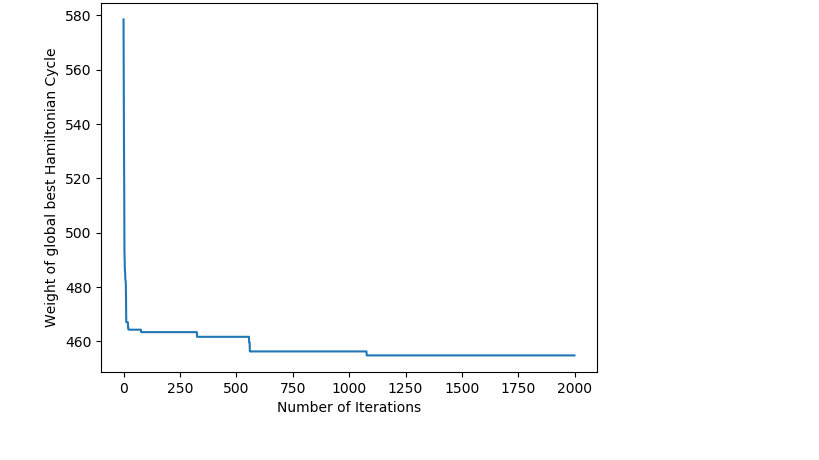
\includegraphics[scale =0.8]{screenshots/screenshot2.png}
\end{figure}
\begin{figure}[H]
   \centering
   \caption{Global Weight Hamiltonian Cycle vs Number of Iterations for gil262}
  \label{plot2}
  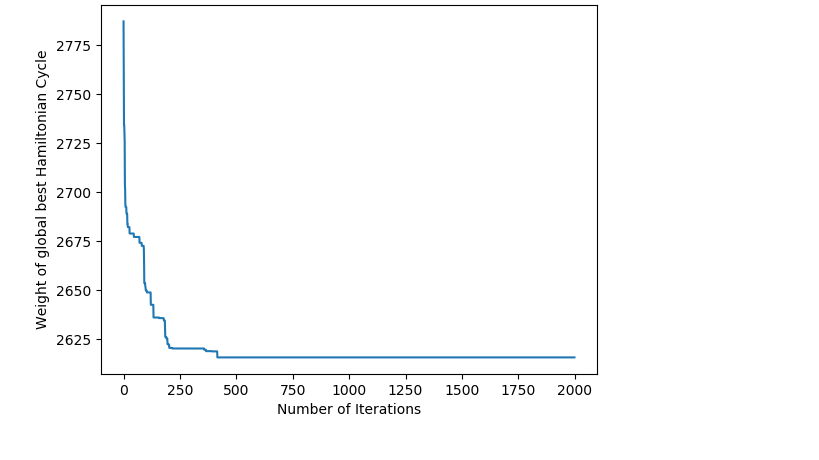
\includegraphics[scale=0.8]{screenshots/screenshot3.png}
\end{figure}
\begin{figure}[H]
  \centering
  \caption{Global Weight Hamiltonian Cycle vs Number of Iterations for pcb442}
  \label{plot3}
  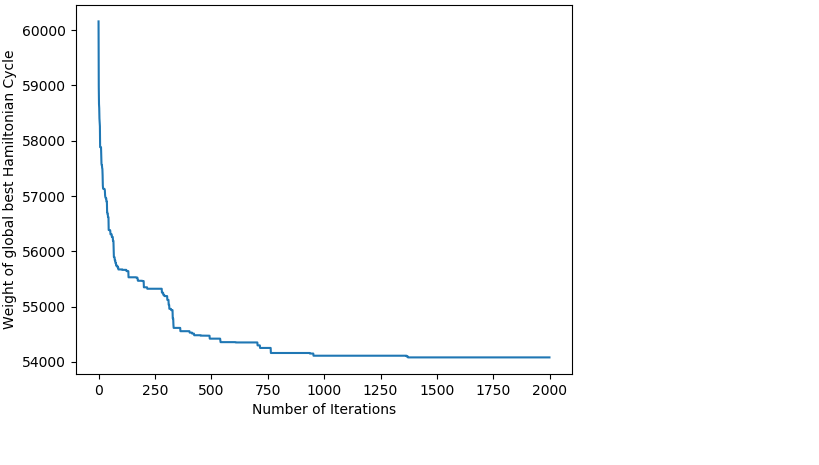
\includegraphics[scale=0.8]{screenshots/screenshot4.png}
\end{figure}
\begin{figure}[H]
  \centering
  \caption{Global Weight Hamiltonian Cycle vs Number of Iterations for p654}
  \label{plot4}
  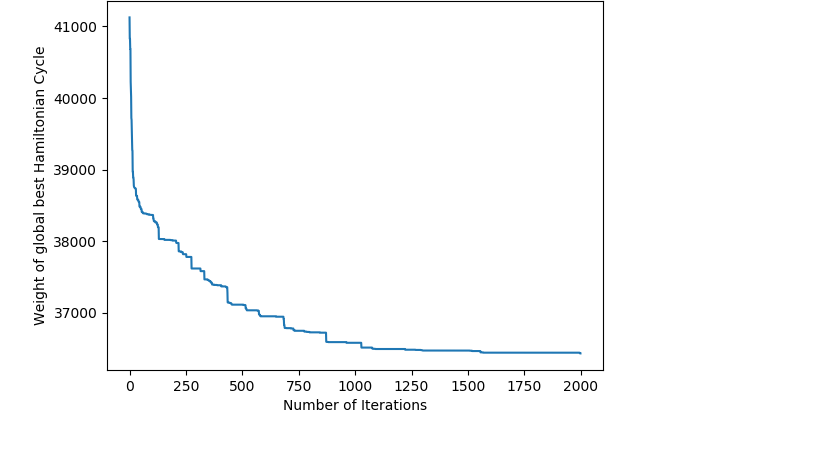
\includegraphics[scale=0.8]{screenshots/screenshot5.png}
\end{figure}
From Figures \ref{plot1}, \ref{plot2}, \ref{plot3}, and \ref{plot4} it can be deduced that the weight of the global best Hamiltonian cycle for instances in ($\real^2$, $d$) decreases towards the optimal value in an exponential manner. In fact, it can be observed from the figures above that when the number of iterations is small, the weight of the global best Hamiltonian cycle decreases at a faster rate compared to when the number of iterations is large. This is reflected in the figures above because, when the number of iterations is small, the curve decreases, but as the number of iterations increase, the curve starts following an asymptotic behavior. This means that as the number of iterations increase, the ACS algorithm will find it harder to find shorter Hamiltonian cycles. Note that, these observations become more evident as the instance size increases.\\\\
The observations described in the previous paragraph have some important consequences. The main consequence is that  since the weight of the global best Hamiltonian cycle for instances in ($\real^2$, $d$) decreases to the optimal value in an exponential manner, then for instances in ($\real^2$, $d$), the ACS algorithm converges in value to the optimal solution in an exponential manner. This means that the ACS algorithm may reach a point where an infeasible amount of time needs to pass for the ACS algorithm to find shorter Hamiltonian cycles. For example, in the blue curve of Figure \ref{plot3} above, a lot of iterations need to be executed after the 750th iteration for the ACS algorithm to find a shorter Hamiltonian cycle, compared to after the 150th iteration. Having empirically analyzed the ACS algorithm, it is now time to compare the approximation results obtained from the empirical analysis of the TAMSA, the NNA, and the ACS algorithm, and deduce whether for instances defined in ($\real^2$, $d$), the ACS algorithm outperforms the NNA and the TAMSA in terms of accuracy of approximations. 
\subsection{Comparison of the Empirical Results of the ACS to those of the TAMSA, and the NNA}
\label{comparison}
Comparing Tables \ref{tab:NNA_results}, \ref{tab:TAMSA_results}, and \ref{tab:ACS_results}, it is evident that in terms of accuracy of approximations, the ACS algorithm outperforms both the TAMSA and the NNA for all the TSP instances in ($\real^2$, $d$) which where chosen. This suggests that for TSP instances defined in ($\real^2$, $d$), the ACS algorithm should be used instead of the TAMSA and the NNA, regardless of the fact that the TAMSA and the NNA have approximation ratios which are known. Therefore for instances in ($\real^2$, $d$), it can be confirmed that it is better in terms of accuracy of approximations to design an algorithm which is guaranteed to find an optimal solution if given enough time, rather than designing an algorithm who's approximation ratio is known (recall the statement made in Section \ref{TAMSA_SECTION}).\\\\
Apart from the fact that the ACS algorithm outperformed both the TAMSA and the NNA in this empirical analysis, it is also good to deduce which algorithm from the TAMSA and the NNA gives the best approximations. From Tables \ref{tab:NNA_results} and \ref{tab:TAMSA_results} it can be deduced that the NNA outperforms the TAMSA in all instances defined in ($\real^2$,$d$) which it was applied to. This result may come as a surprise because, the NNA's approximation ratio increases logarithmically with respect to the instance size unlike that of the TAMSA which is constant. It is important to note that this result may only be true because, the TAMSA and the NNA where optimized as discussed in Sections \ref{tamsa_analysis} and \ref{NNA_analyze} to return the best result possible. Hence, it may be the case that if not optimized, the TAMSA may give better results on average than the NNA. However, regardless of this, the empirical results suggest that for instances in ($\real^2$, $d$), the NNA at best will give better approximations compared to the TAMSA.
%sort style alphabetical
%remove spacing in cites
\newpage
\section{Conclusion}
\newpage
\bibliography{bibliography}
\bibliographystyle{Ieeetran} %have to be changed to APA
\end{document}